\chapter{RESULTADOS}
\label{cap:resultados}

Este capítulo reporta los resultados de los casos de prueba P1 a P4 del
plan de pruebas (Sección~\ref{sec:plan}) sobre los escenarios sintéticos
de la Tabla~\ref{tab:escenarios} y, en la
Sección~\ref{sec:resultados-u4}, los del módulo U4 (casos P3-U4, P4-U4
y P6, más la prueba de humo en el cruce). Para cada caso se presentan
las entradas y salidas por episodio de entrenamiento, la evaluación
final con la política congelada sobre diez semillas comunes a todos los
controles, y las figuras que resumen el aprendizaje y la comparación. Todas las tablas
y figuras se generan con los scripts del proyecto a partir de los
archivos de resultados (\texttt{tablas\_tex.py} y \texttt{graficar.py});
las tablas completas por episodio están en el Anexo~A.

\section{Resumen de los cuatro casos}

La Tabla~\ref{tab:resumen-escenarios} reúne la métrica primaria de los
cuatro casos. El agente Q-learning reduce el retraso frente al tiempo
fijo tuneado solo en el cruce de dos fases ($-6$\,\%) y lo aumenta en
los otros tres casos: $+15$\,\% en la red de tres cruces con onda
verde, $+17$\,\% en el cruce con giros protegidos y $+60$\,\% en el
corredor de dos cruces. Los fijos de corredor y red se retunearon con
reparto de verde asimétrico (Sección~\ref{sec:escenarios}); frente a
los fijos simétricos originales las pérdidas eran de $+6$ y $+13$\,\%.
En ningún caso alcanza la meta de $-25$\,\%. El control actuado nativo
de SUMO, con los mismos límites de verde que el agente, es mejor que el
fijo en tres casos (de $-2$\,\% en red a $-33$\,\% en cruce), empata
con el fijo tuneado del corredor y es mejor que el agente en los
cuatro.

% Generado por tablas_tex.py a partir de los CSV del proyecto. No editar a mano.
\begin{table}[H]
\setstretch{1}
\centering
\scriptsize
\setlength{\tabcolsep}{3pt}
\begin{tabular}{lrrrrrrrrr}
\toprule
 & \multicolumn{3}{c}{Retraso (s/veh)} & \multicolumn{2}{c}{RL vs fijo} & Actuado & \multicolumn{3}{c}{RL vs fijo, secundarias} \\
\cmidrule(lr){2-4}\cmidrule(lr){5-6}\cmidrule(lr){7-7}\cmidrule(lr){8-10}
Escenario & Fijo & Actuado & RL & $\Delta$ [IC95\,\%] & $p$ & $\Delta$ vs fijo & Espera & Paradas & CO$_2$ \\
\midrule
cruce & 23.19 & 15.46 & 21.72 & $-$6.4\,\% [$-$9.3, $-$2.7] & 0.0137 & $-$33.4\,\% & $-$25.9\,\% & +27.4\,\% & $-$1.5\,\% \\
cruce2 & 27.54 & 23.21 & 32.15 & +16.7\,\% [9.9, 25.4] & 0.00195 & $-$15.7\,\% & +18.4\,\% & +23.5\,\% & +4.0\,\% \\
corredor & 31.86 & 20.91 & 33.86 & +6.3\,\% [1.3, 11.0] & 0.0371 & $-$34.4\,\% & $-$13.5\,\% & +49.3\,\% & +1.3\,\% \\
red & 22.22 & 21.42 & 25.12 & +13.1\,\% [12.0, 14.1] & 0.00195 & $-$3.6\,\% & +3.6\,\% & +74.1\,\% & +5.3\,\% \\
\bottomrule
\end{tabular}
\caption[Resumen por escenario]{Resumen por escenario: retraso promedio por vehículo con política congelada, 10 semillas de evaluación comunes a los tres controles. La meta de la tesis es $-25\,\%$ de retraso frente al fijo.}
\label{tab:resumen-escenarios}
\end{table}


Tres regularidades atraviesan los cuatro casos y se desarrollan en la
Sección~\ref{sec:lectura}. La espera detenida, que es la señal de la
recompensa, sale mejor parada que el retraso: baja más que él donde el
retraso baja (cruce, $-26$ contra $-6$\,\%) y en red sube mucho menos
que él ($+4$ contra $+15$\,\%); en cruce2, donde la política es
inestable, empeoran las dos por igual, y en corredor, frente al fijo
tuneado, empeoran las dos. El agente cambia de fase entre un $13$ y un
$77$\,\% más que el fijo y en los cuatro casos aumenta las paradas por
vehículo.
Y su desempeño se degrada cuando crece el espacio de estados o cuando
hay varios semáforos consecutivos.

\section{Caso P1: cruce de dos fases}

La Tabla~\ref{tab:cruce-episodios-resumen} muestra los parámetros de
entrada y las métricas de salida de episodios escogidos del
entrenamiento (la tabla completa de los 40 episodios está en el Anexo~A).
Las columnas de entrada son las únicas que cambian entre episodios: la
probabilidad de exploración $\varepsilon$, la semilla de SUMO y el número
de estados que la tabla Q ya conocía al empezar. Red, demanda, pesos de
la recompensa e hiperparámetros son idénticos en las 40 filas.

% Generado por tablas_tex.py a partir de los CSV del proyecto. No editar a mano.
\begin{table}[H]
\setstretch{1}
\centering
\scriptsize
\setlength{\tabcolsep}{3pt}
\begin{tabular}{rrrrrrrrrrrr}
\toprule
\multicolumn{4}{c}{Entradas del episodio} & \multicolumn{6}{c}{Salidas del episodio (entrenamiento, $\varepsilon>0$)} & \multicolumn{2}{c}{Política congelada} \\
\cmidrule(lr){1-4}\cmidrule(lr){5-10}\cmidrule(lr){11-12}
Ep. & $\varepsilon$ & Semilla & Q ini. & Retraso & Espera & Cola & $r$/dec. & Cambios & Paradas & Retraso & Espera \\
 &  &  & (estados) & (s/veh) & (s/veh) & (veh) &  & de fase & (/veh) & (s/veh) & (s/veh) \\
\midrule
fijo & 0 & 42 & -- & 22.83 & 9.30 & 5.16 & $-$5.58 & 131 & 0.67 & -- & -- \\
\midrule
1 & 1.000 & 43 & 0 & 80.14 & 30.84 & 14.82 & $-$15.98 & 227 & 3.16 & -- & -- \\
2 & 0.900 & 44 & 81 & 51.59 & 21.21 & 10.90 & $-$11.64 & 219 & 2.16 & -- & -- \\
3 & 0.810 & 45 & 104 & 36.22 & 15.46 & 7.97 & $-$8.51 & 215 & 1.43 & -- & -- \\
5 & 0.656 & 47 & 119 & 31.21 & 12.33 & 6.62 & $-$7.00 & 222 & 1.27 & 22.15 & 7.26 \\
10 & 0.387 & 52 & 123 & 27.00 & 9.95 & 5.45 & $-$5.72 & 222 & 1.09 & 21.43 & 7.43 \\
15 & 0.229 & 57 & 124 & 22.18 & 7.45 & 4.23 & $-$4.41 & 227 & 0.89 & 20.13 & 6.28 \\
20 & 0.135 & 62 & 126 & 22.10 & 7.59 & 4.31 & $-$4.48 & 229 & 0.88 & 39.18 & 12.66 \\
25 & 0.080 & 67 & 127 & 19.42 & 6.24 & 3.62 & $-$3.75 & 213 & 0.72 & 20.50 & 6.56 \\
30 & 0.050 & 72 & 129 & 17.80 & 5.31 & 3.16 & $-$3.30 & 215 & 0.64 & 19.62 & 6.18 \\
35 & 0.050 & 77 & 130 & 19.66 & 6.23 & 3.62 & $-$3.76 & 219 & 0.74 & 20.02 & 6.36 \\
40 & 0.050 & 82 & 130 & 21.65 & 7.13 & 4.07 & $-$4.23 & 223 & 0.84 & 21.39 & 7.05 \\
\bottomrule
\end{tabular}
\caption[Escenario cruce: episodios de entrenamiento]{Escenario cruce: parámetros de entrada y métricas de salida por episodio. 40 episodios de entrenamiento con semilla base 42; la fila fijo es el tiempo fijo con la misma semilla base. La política congelada se evalúa cada 5 episodios con una semilla fija ajena al entrenamiento y a la evaluación final. Se muestran episodios escogidos; la tabla completa está en el Anexo~A.}
\label{tab:cruce-episodios-resumen}
\end{table}



La Figura~\ref{fig:cruce-curva} muestra el mismo proceso: cada punto gris
es una hora completa de tráfico bajo el agente en entrenamiento; el
retraso baja de 80~s por vehículo en el primer episodio, con
$\varepsilon = 1$ y decisiones al azar, a unos 22~s desde el episodio~15
(21~s en los últimos diez), y a partir del episodio~30, cuando
$\varepsilon$ toca el piso de 0.05, la oscilación restante es del mismo
orden que la diferencia entre semillas. La política congelada
(marcadores verdes, semilla fija 999) se sitúa por debajo de la banda
del tiempo fijo desde el episodio~5, con una excepción en el
episodio~20, y muy por encima de la línea del actuado.
La tabla Q termina con 130 estados visitados de 512 posibles y el mayor
cambio de un valor Q por episodio se estabiliza desde el episodio~10
(Figura~\ref{fig:cruce-qtable}).

\begin{figure}[H]
  \centering
  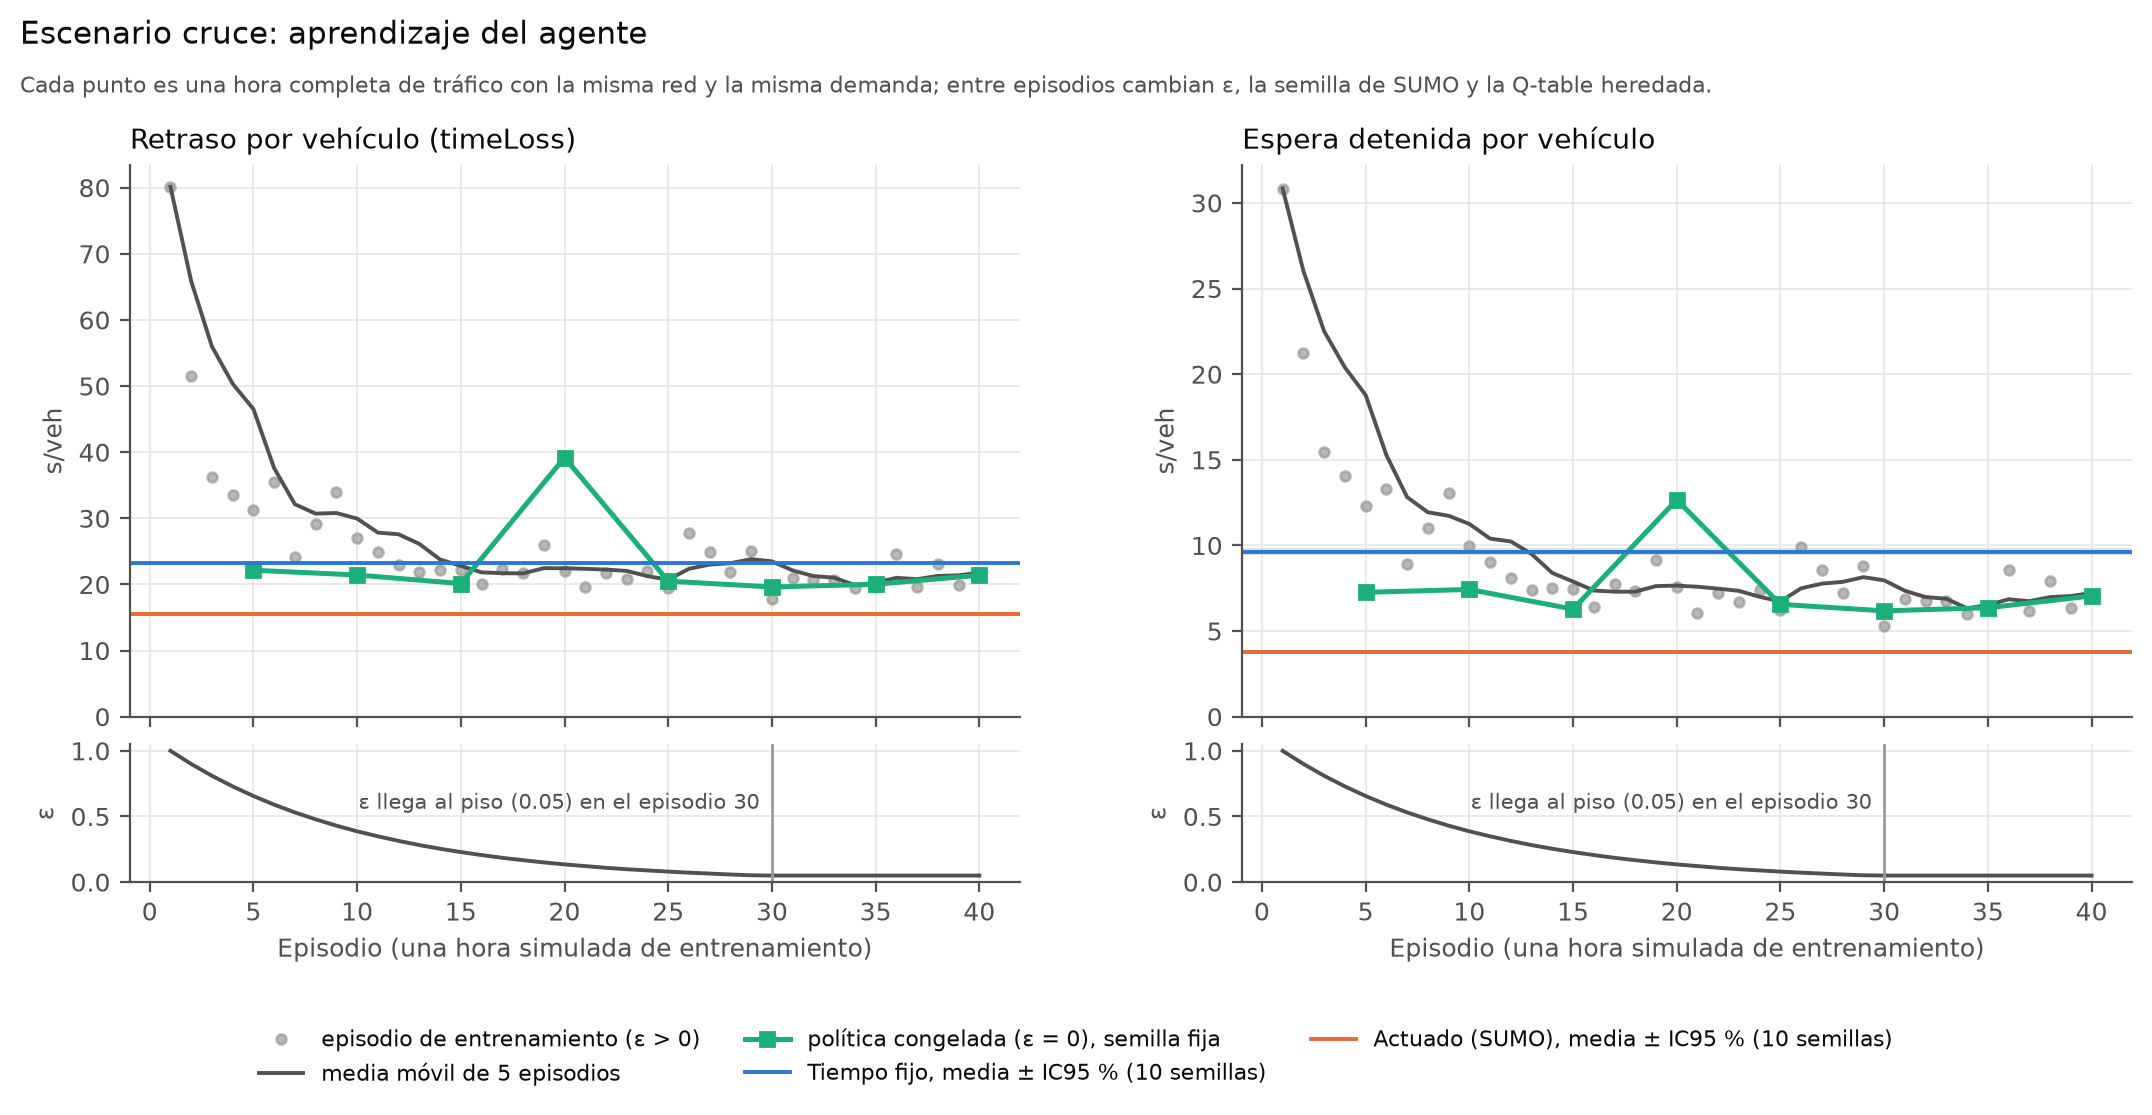
\includegraphics[width=\textwidth]{fig_cruce_curva.png}
  \caption{Escenario cruce: retraso y espera detenida por episodio de entrenamiento (puntos grises y media móvil), evaluación de la política congelada cada cinco episodios (verde), tiempo fijo (azul) y actuado (naranja) como media $\pm$ IC95\,\% sobre las diez semillas de evaluación. Debajo, el valor de $\varepsilon$ de cada episodio.}
  \label{fig:cruce-curva}
\end{figure}

\begin{figure}[H]
  \centering
  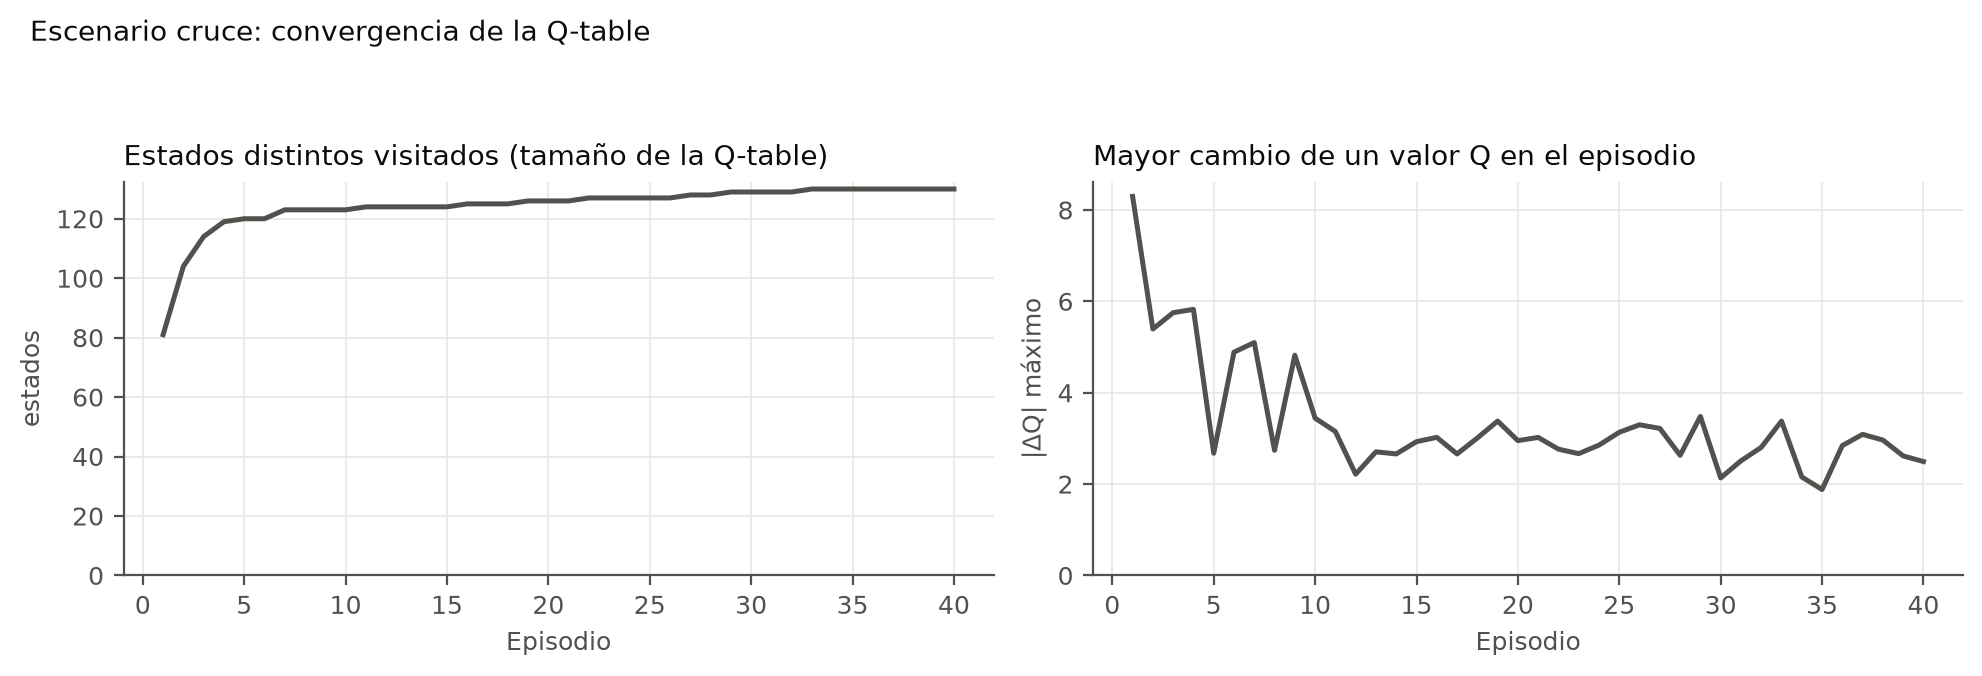
\includegraphics[width=\textwidth]{fig_cruce_qtable.png}
  \caption{Escenario cruce: estados distintos visitados por la tabla Q y mayor cambio de un valor Q en cada episodio.}
  \label{fig:cruce-qtable}
\end{figure}

La evaluación final (Tabla~\ref{tab:cruce-evaluacion} y
Figura~\ref{fig:cruce-comparacion}) se hizo con la política congelada
sobre las semillas 1001 a 1010. El agente reduce el retraso un
$6.4$\,\% frente al fijo (intervalo $-9.3$ a $-2.7$\,\%, $p = 0.014$),
la espera detenida un $26$\,\% y la cola promedio un $23$\,\%, pero
aumenta las paradas por vehículo un $27$\,\% y deja la cola máxima igual.
La explicación está en los cambios de fase: 233 por hora frente a 131
del fijo. El agente corta el verde en cuanto la cola del eje en rojo
supera a la del eje en verde, lo que acorta las esperas pero obliga a
más vehículos a frenar y volver a arrancar; el retraso, que incluye esas
frenadas y aceleraciones, mejora mucho menos que la espera. La reducción
de CO$_2$ es de $1.5$\,\%. El actuado, con las mismas fases y los mismos
límites de verde, reduce el retraso un $33$\,\% y la espera un $61$\,\%
con menos paradas que el fijo.

% Generado por tablas_tex.py a partir de los CSV del proyecto. No editar a mano.
\begin{table}[H]
\setstretch{1}
\centering
\scriptsize
\setlength{\tabcolsep}{3pt}
\begin{tabular}{lrrrrrr}
\toprule
Métrica & Tiempo fijo & Actuado & Q-learning & \makecell{$\Delta$ RL vs fijo\\{}[IC95\,\%]} & $p$ & \makecell{$\Delta$ actuado\\vs fijo} \\
\midrule
Retraso (s/veh) & 23.19 $\pm$ 0.25 & 15.46 $\pm$ 0.18 & 21.72 $\pm$ 1.00 & $-$6.4\,\% [$-$9.3, $-$2.7] & 0.0137 & $-$33.4\,\% \\
Espera detenida (s/veh) & 9.63 $\pm$ 0.20 & 3.79 $\pm$ 0.05 & 7.14 $\pm$ 0.49 & $-$25.9\,\% [$-$29.9, $-$21.1] & 0.00195 & $-$60.7\,\% \\
Cola promedio (veh) & 5.31 $\pm$ 0.10 & 2.40 $\pm$ 0.03 & 4.07 $\pm$ 0.23 & $-$23.5\,\% [$-$26.8, $-$19.3] & 0.00195 & $-$54.8\,\% \\
Cola máxima (veh) & 18.00 $\pm$ 0.67 & 11.50 $\pm$ 0.77 & 18.40 $\pm$ 0.69 & +2.2\,\% [$-$0.5, 5.1] & 0.312 & $-$36.1\,\% \\
Paradas por vehículo & 0.68 $\pm$ 0.01 & 0.49 $\pm$ 0.01 & 0.87 $\pm$ 0.05 & +27.4\,\% [21.5, 34.1] & 0.00195 & $-$27.8\,\% \\
Throughput (veh) & 1802.00 $\pm$ 1.26 & 1807.50 $\pm$ 0.84 & 1802.70 $\pm$ 3.00 & +0.0\,\% [$-$0.1, 0.2] & 0.766 & +0.3\,\% \\
CO$_2$ (g/veh) & 196.11 $\pm$ 0.55 & 180.54 $\pm$ 0.47 & 193.13 $\pm$ 1.84 & $-$1.5\,\% [$-$2.2, $-$0.8] & 0.00977 & $-$7.9\,\% \\
NO$_x$ (mg/veh) & 67.34 $\pm$ 0.19 & 61.72 $\pm$ 0.13 & 65.97 $\pm$ 0.64 & $-$2.0\,\% [$-$2.7, $-$1.3] & 0.00391 & $-$8.3\,\% \\
Recompensa por decisión & $-$5.74 $\pm$ 0.12 & $-$2.48 $\pm$ 0.03 & $-$4.23 $\pm$ 0.26 & $-$26.4\,\% [$-$29.8, $-$22.2] & 0.00195 & $-$56.8\,\% \\
Cambios de fase & 131.40 $\pm$ 0.37 & 203.00 $\pm$ 2.02 & 232.70 $\pm$ 3.66 & +77.1\,\% [74.4, 79.2] & 0.00195 & +54.5\,\% \\
\bottomrule
\end{tabular}
\caption[Escenario cruce: evaluación con política congelada]{Escenario cruce: evaluación con política congelada sobre 10 semillas (1001 a 1010), las mismas para los tres controles. Media $\pm$ IC95\,\%; el cambio porcentual lleva su intervalo bootstrap pareado y $p$ es el de la prueba de Wilcoxon pareada frente al fijo.}
\label{tab:cruce-evaluacion}
\end{table}


\begin{figure}[H]
  \centering
  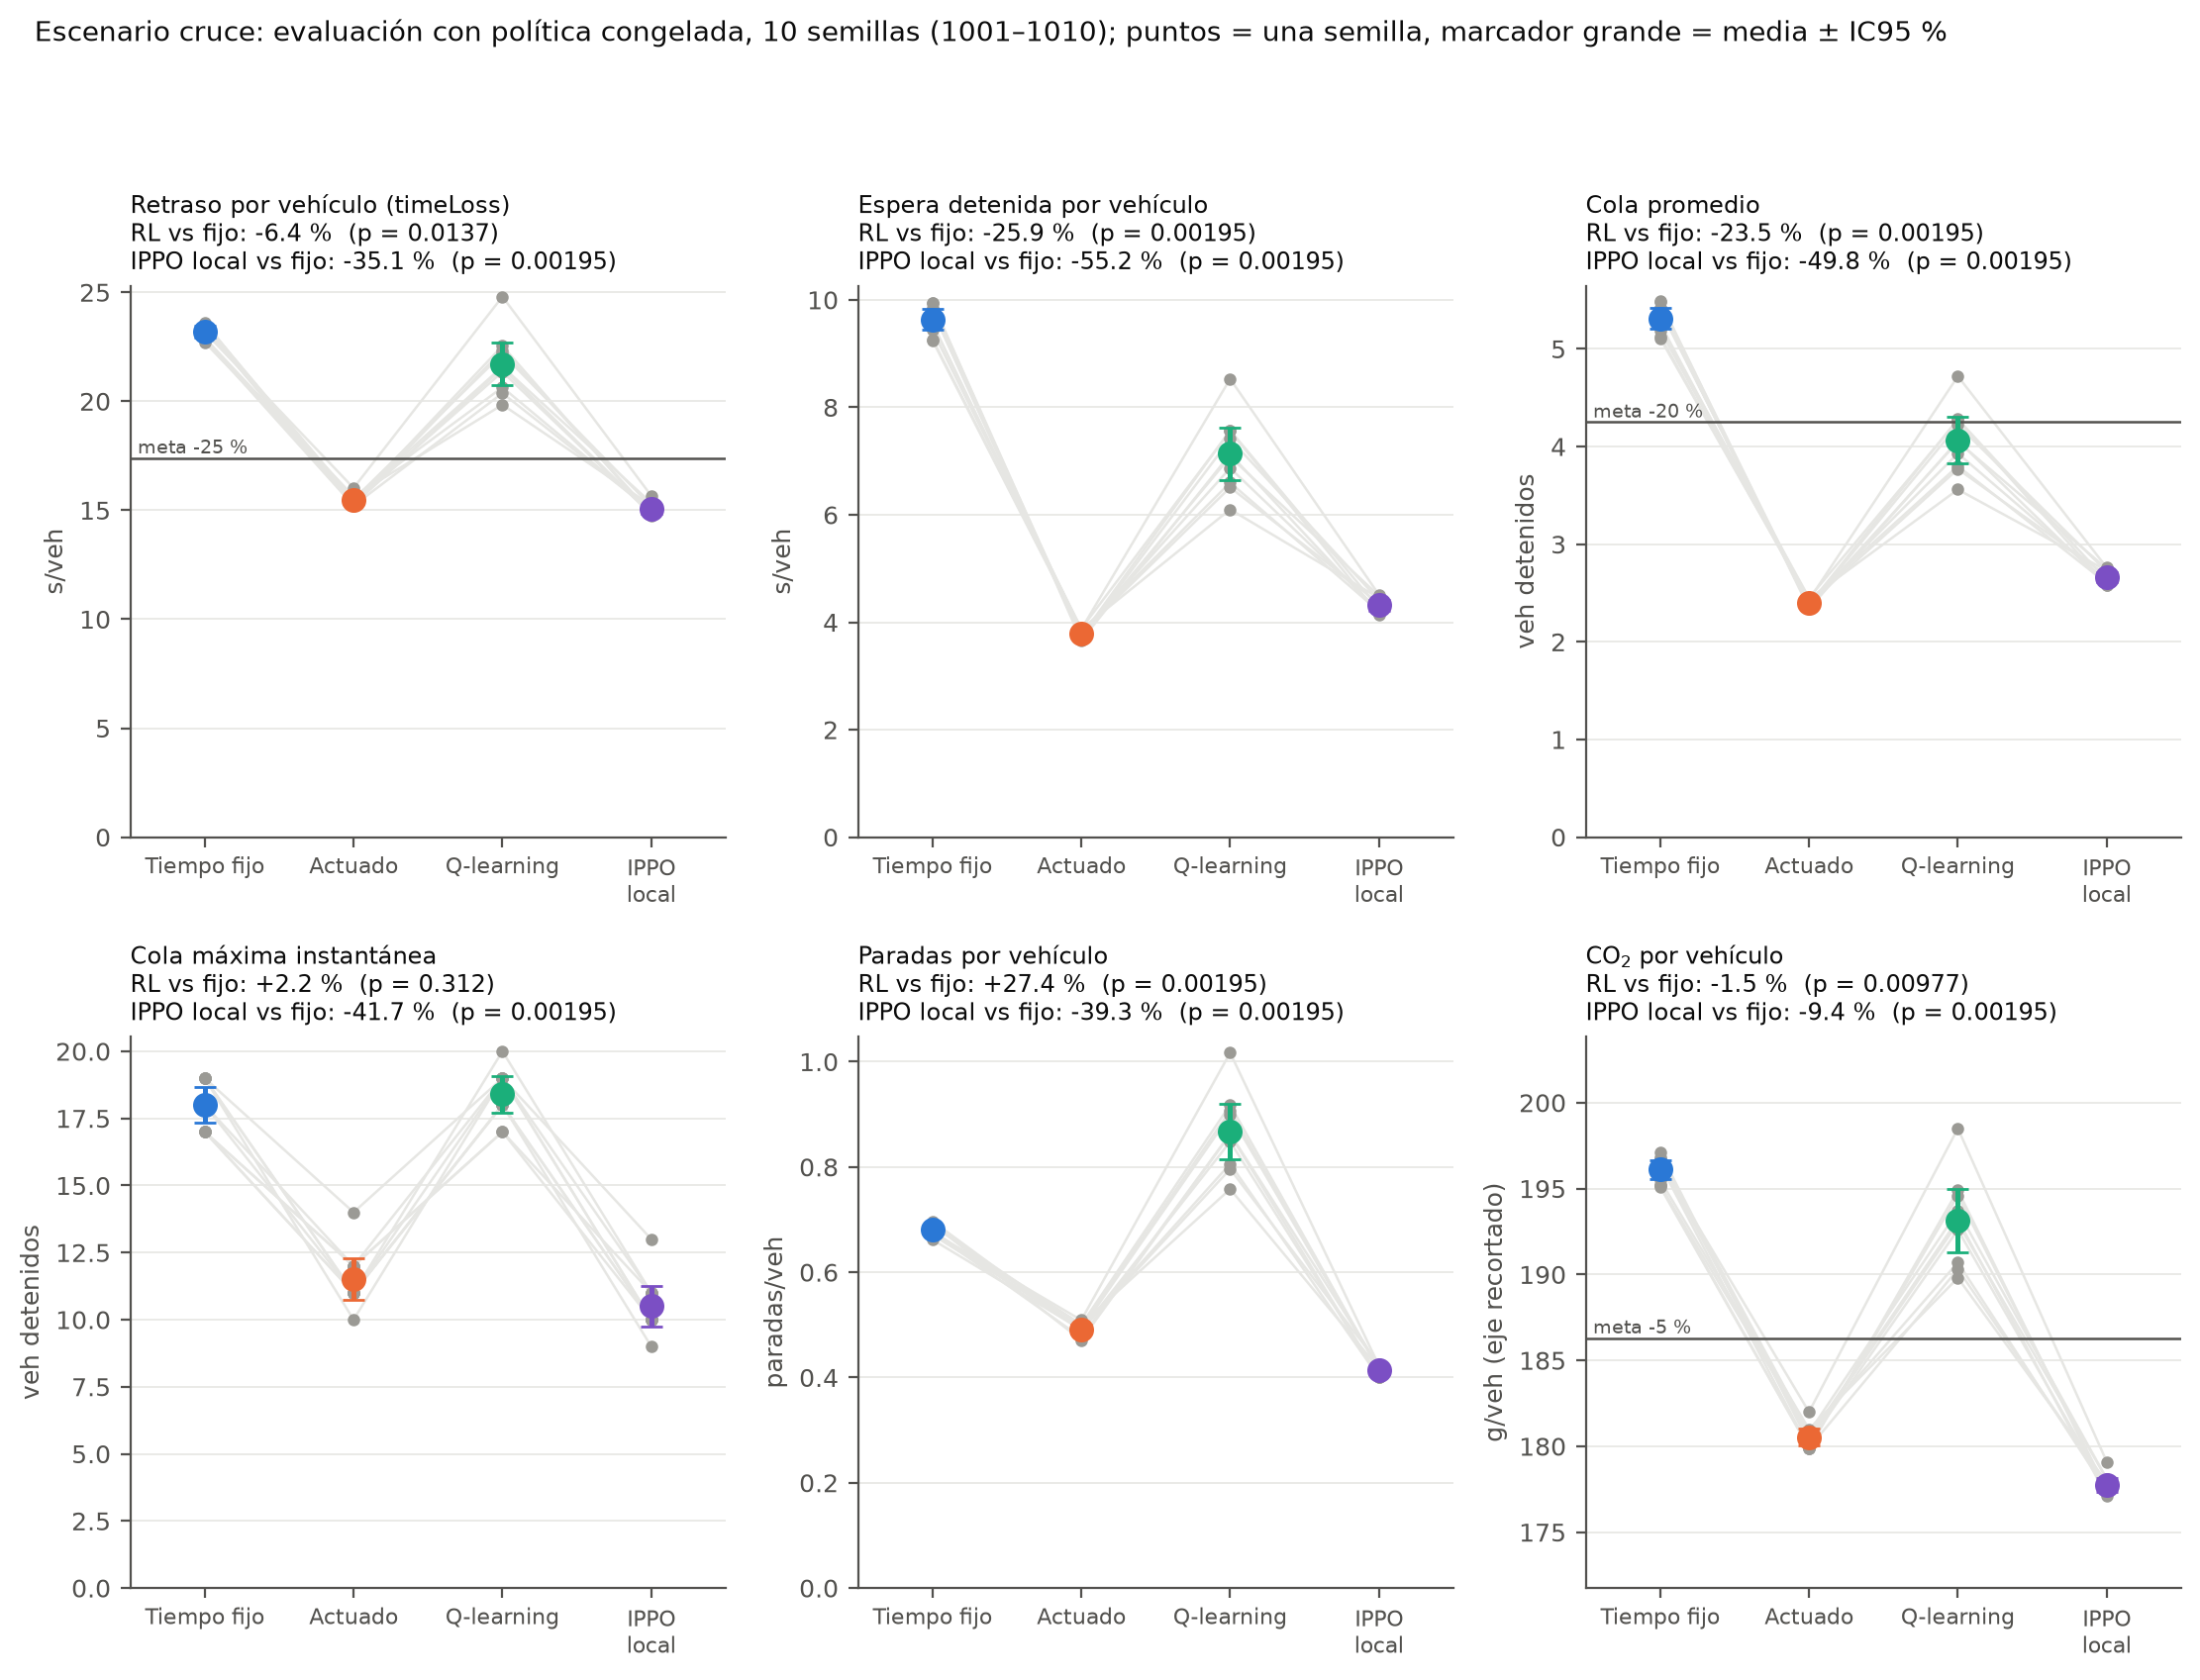
\includegraphics[width=\textwidth]{fig_cruce_comparacion.png}
  \caption{Escenario cruce: cada punto gris es una semilla de evaluación y las líneas unen la misma semilla bajo los tres controles; el marcador grande es la media con su IC95\,\%. La línea horizontal marca la meta de la tesis respecto al fijo.}
  \label{fig:cruce-comparacion}
\end{figure}

La Figura~\ref{fig:cruce-serie} muestra qué hace cada control dentro de
la hora, con la misma semilla. Bajo el tiempo fijo el eje N--S acumula
colas de hasta 16 vehículos en la primera media hora, cuando lleva la
punta, y el eje E--O en la segunda; el agente reparte el verde según la
cola que observa y mantiene ambos ejes por debajo de 10 vehículos la
mayor parte del tiempo, a costa de picos breves; el actuado mantiene las
colas más bajas y más estables. La distribución por vehículo
(Figura~\ref{fig:cruce-ecdf}) confirma que el agente mueve toda la
distribución del retraso hacia la izquierda respecto al fijo y que el
percentil 90 baja de 36.5 a 32.5~s.

\begin{figure}[H]
  \centering
  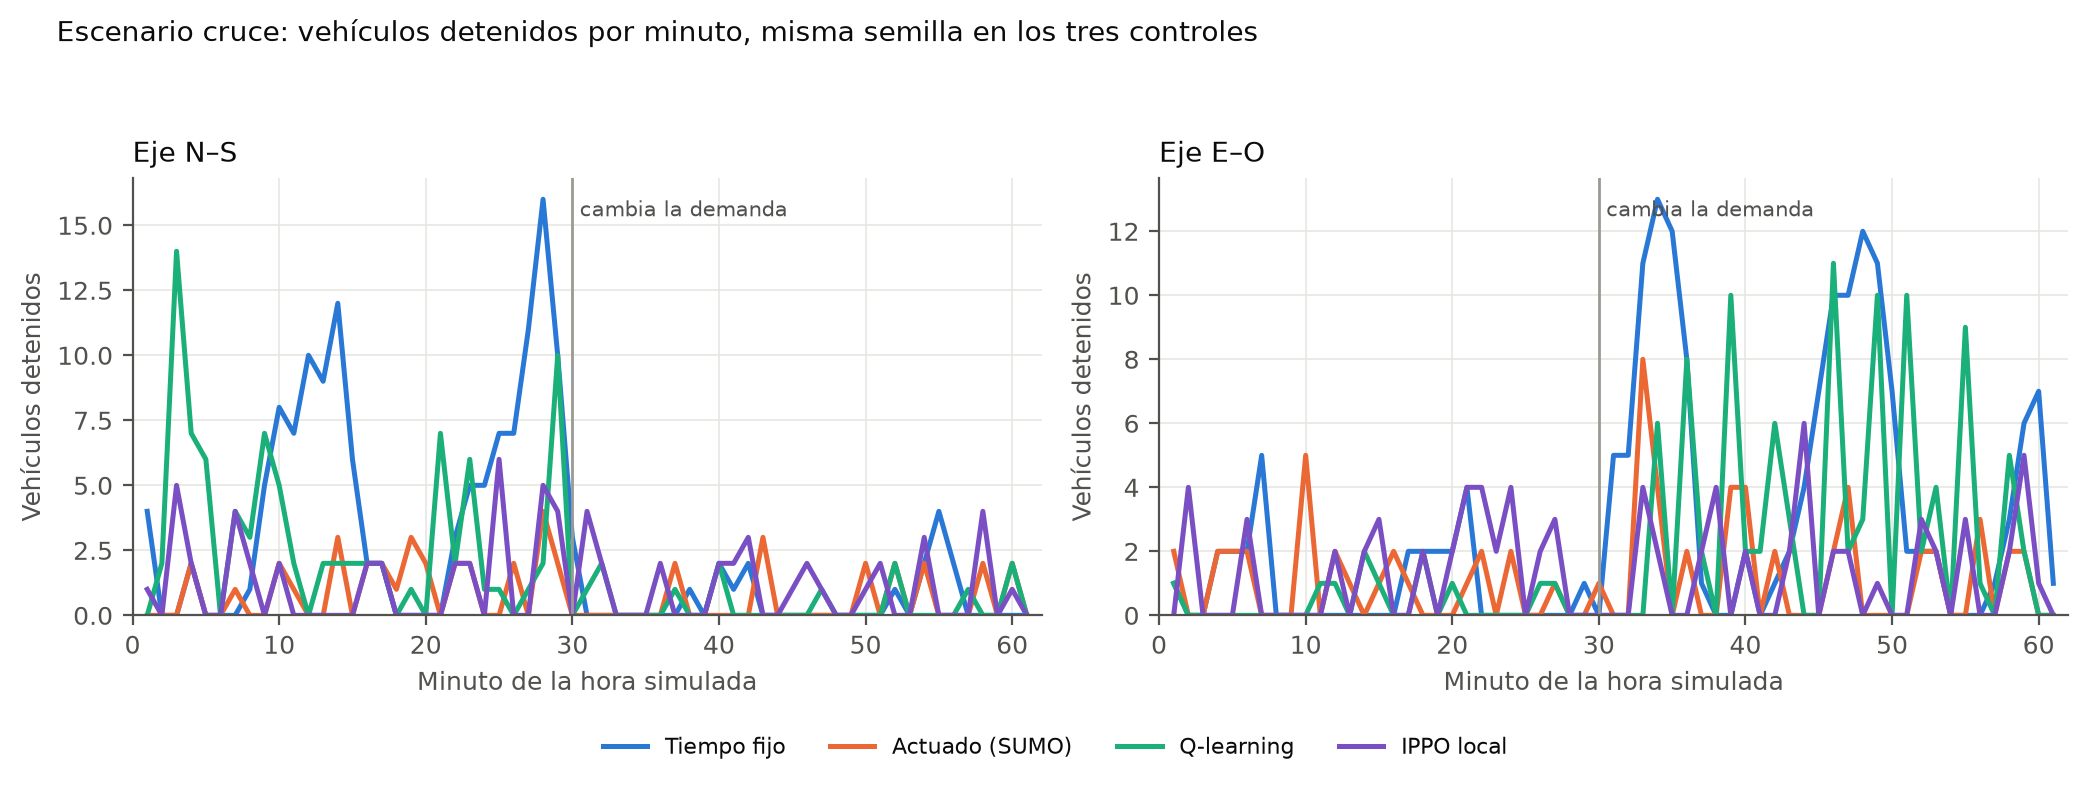
\includegraphics[width=\textwidth]{fig_cruce_serie.png}
  \caption{Escenario cruce: vehículos detenidos por minuto en cada eje bajo los tres controles, semilla 1001. La línea vertical marca la inversión de la demanda a los 30 minutos.}
  \label{fig:cruce-serie}
\end{figure}

\begin{figure}[H]
  \centering
  
\includegraphics[width=\textwidth]{fig_cruce_ecdf.png}
  \caption{Escenario cruce: distribución acumulada del retraso y de la espera detenida por vehículo, semilla 1001; el punto marca el percentil 90 de cada control.}
  \label{fig:cruce-ecdf}
\end{figure}

\section{Caso P2: cruce con giros protegidos}

Con cuatro fases verdes el espacio de estados crece a 1024 y el agente
necesitó un decaimiento más lento de $\varepsilon$ (0.96) y 120
episodios; $\varepsilon$ toca el piso en el episodio~75
(Tabla~\ref{tab:cruce2-episodios-resumen}, Figura~\ref{fig:cruce2-curva}).
Durante el entrenamiento, con exploración residual, el agente iguala al
tiempo fijo; con la política congelada queda por encima de él en 14 de
las 24 evaluaciones intermedias y, en cinco de ellas (episodios 5, 10,
60, 75 y 120), la política se bloquea con la semilla de evaluación y el
retraso sube a entre 47 y 210~s. Al terminar, la tabla Q conoce 390
estados de 1024 (Figura~\ref{fig:cruce2-qtable}): más de la mitad del
espacio nunca se visitó y, en los estados poco visitados, la política
greedy elige entre valores apenas actualizados.

% Generado por tablas_tex.py a partir de los CSV del proyecto. No editar a mano.
\begin{table}[H]
\setstretch{1}
\centering
\scriptsize
\setlength{\tabcolsep}{3pt}
\begin{tabular}{rrrrrrrrrrrr}
\toprule
\multicolumn{4}{c}{Entradas del episodio} & \multicolumn{6}{c}{Salidas del episodio (entrenamiento, $\varepsilon>0$)} & \multicolumn{2}{c}{Política congelada} \\
\cmidrule(lr){1-4}\cmidrule(lr){5-10}\cmidrule(lr){11-12}
Ep. & $\varepsilon$ & Semilla & Q ini. & Retraso & Espera & Cola & $r$/dec. & Cambios & Paradas & Retraso & Espera \\
 &  &  & (estados) & (s/veh) & (s/veh) & (veh) &  & de fase & (/veh) & (s/veh) & (s/veh) \\
\midrule
fijo & 0 & 42 & -- & 27.94 & 15.96 & 7.69 & $-$8.36 & 230 & 0.89 & -- & -- \\
\midrule
1 & 1.000 & 43 & 0 & 207.74 & 132.44 & 57.32 & $-$67.25 & 280 & 6.91 & -- & -- \\
2 & 0.960 & 44 & 106 & 207.37 & 134.95 & 57.69 & $-$67.97 & 296 & 6.30 & -- & -- \\
3 & 0.922 & 45 & 128 & 154.32 & 99.04 & 47.59 & $-$56.27 & 256 & 4.74 & -- & -- \\
5 & 0.849 & 47 & 199 & 89.60 & 59.52 & 28.76 & $-$34.10 & 245 & 2.27 & 209.53 & 153.51 \\
10 & 0.693 & 52 & 282 & 106.36 & 67.16 & 31.43 & $-$36.27 & 280 & 3.01 & 48.71 & 30.97 \\
15 & 0.565 & 57 & 328 & 40.80 & 25.90 & 12.70 & $-$14.39 & 256 & 1.19 & 26.65 & 15.05 \\
20 & 0.460 & 62 & 355 & 38.80 & 23.88 & 11.77 & $-$13.10 & 271 & 1.20 & 33.96 & 20.13 \\
25 & 0.375 & 67 & 362 & 32.77 & 19.28 & 9.47 & $-$10.39 & 265 & 1.06 & 32.32 & 18.48 \\
30 & 0.306 & 72 & 372 & 31.39 & 18.35 & 9.02 & $-$9.90 & 266 & 1.03 & 37.14 & 21.75 \\
35 & 0.250 & 77 & 375 & 28.95 & 16.68 & 8.09 & $-$8.90 & 244 & 0.93 & 26.18 & 14.52 \\
40 & 0.204 & 82 & 378 & 27.71 & 15.55 & 7.56 & $-$8.22 & 255 & 0.93 & 26.06 & 14.63 \\
45 & 0.166 & 87 & 382 & 31.11 & 18.07 & 8.84 & $-$9.68 & 271 & 1.01 & 26.33 & 14.88 \\
50 & 0.135 & 92 & 383 & 27.64 & 15.66 & 7.59 & $-$8.32 & 248 & 0.90 & 34.65 & 20.20 \\
55 & 0.110 & 97 & 384 & 27.12 & 15.23 & 7.46 & $-$8.11 & 248 & 0.91 & 32.38 & 18.73 \\
60 & 0.090 & 102 & 385 & 28.06 & 15.84 & 7.75 & $-$8.46 & 262 & 0.94 & 47.35 & 28.86 \\
65 & 0.073 & 107 & 386 & 29.27 & 16.66 & 7.81 & $-$8.55 & 271 & 0.97 & 25.62 & 14.21 \\
70 & 0.060 & 112 & 387 & 26.78 & 14.92 & 7.26 & $-$7.91 & 235 & 0.89 & 25.90 & 14.28 \\
75 & 0.050 & 117 & 387 & 24.92 & 13.57 & 6.57 & $-$7.10 & 239 & 0.83 & 68.64 & 45.86 \\
80 & 0.050 & 122 & 387 & 28.91 & 16.40 & 8.10 & $-$8.80 & 254 & 0.96 & 32.55 & 19.02 \\
85 & 0.050 & 127 & 388 & 25.53 & 14.12 & 6.83 & $-$7.43 & 234 & 0.84 & 25.50 & 14.01 \\
90 & 0.050 & 132 & 389 & 26.26 & 14.46 & 7.03 & $-$7.64 & 253 & 0.88 & 31.05 & 17.48 \\
95 & 0.050 & 137 & 390 & 29.78 & 17.11 & 8.33 & $-$9.12 & 249 & 0.97 & 25.27 & 13.99 \\
100 & 0.050 & 142 & 390 & 26.94 & 15.05 & 7.39 & $-$8.08 & 245 & 0.90 & 25.28 & 13.99 \\
105 & 0.050 & 147 & 390 & 27.42 & 15.49 & 7.54 & $-$8.26 & 237 & 0.89 & 30.19 & 17.22 \\
110 & 0.050 & 152 & 390 & 25.45 & 14.10 & 6.83 & $-$7.49 & 224 & 0.82 & 29.60 & 16.72 \\
115 & 0.050 & 157 & 390 & 25.99 & 14.40 & 7.06 & $-$7.66 & 237 & 0.85 & 25.72 & 14.36 \\
120 & 0.050 & 162 & 390 & 26.53 & 14.81 & 7.19 & $-$7.84 & 238 & 0.87 & 179.00 & 134.62 \\
\bottomrule
\end{tabular}
\caption[Escenario cruce2: episodios de entrenamiento]{Escenario cruce2: parámetros de entrada y métricas de salida por episodio. 120 episodios de entrenamiento con semilla base 42; la fila fijo es el tiempo fijo con la misma semilla base. La política congelada se evalúa cada 5 episodios con una semilla fija ajena al entrenamiento y a la evaluación final. Se muestran episodios escogidos; la tabla completa está en el Anexo~A.}
\label{tab:cruce2-episodios-resumen}
\end{table}



\begin{figure}[H]
  \centering
  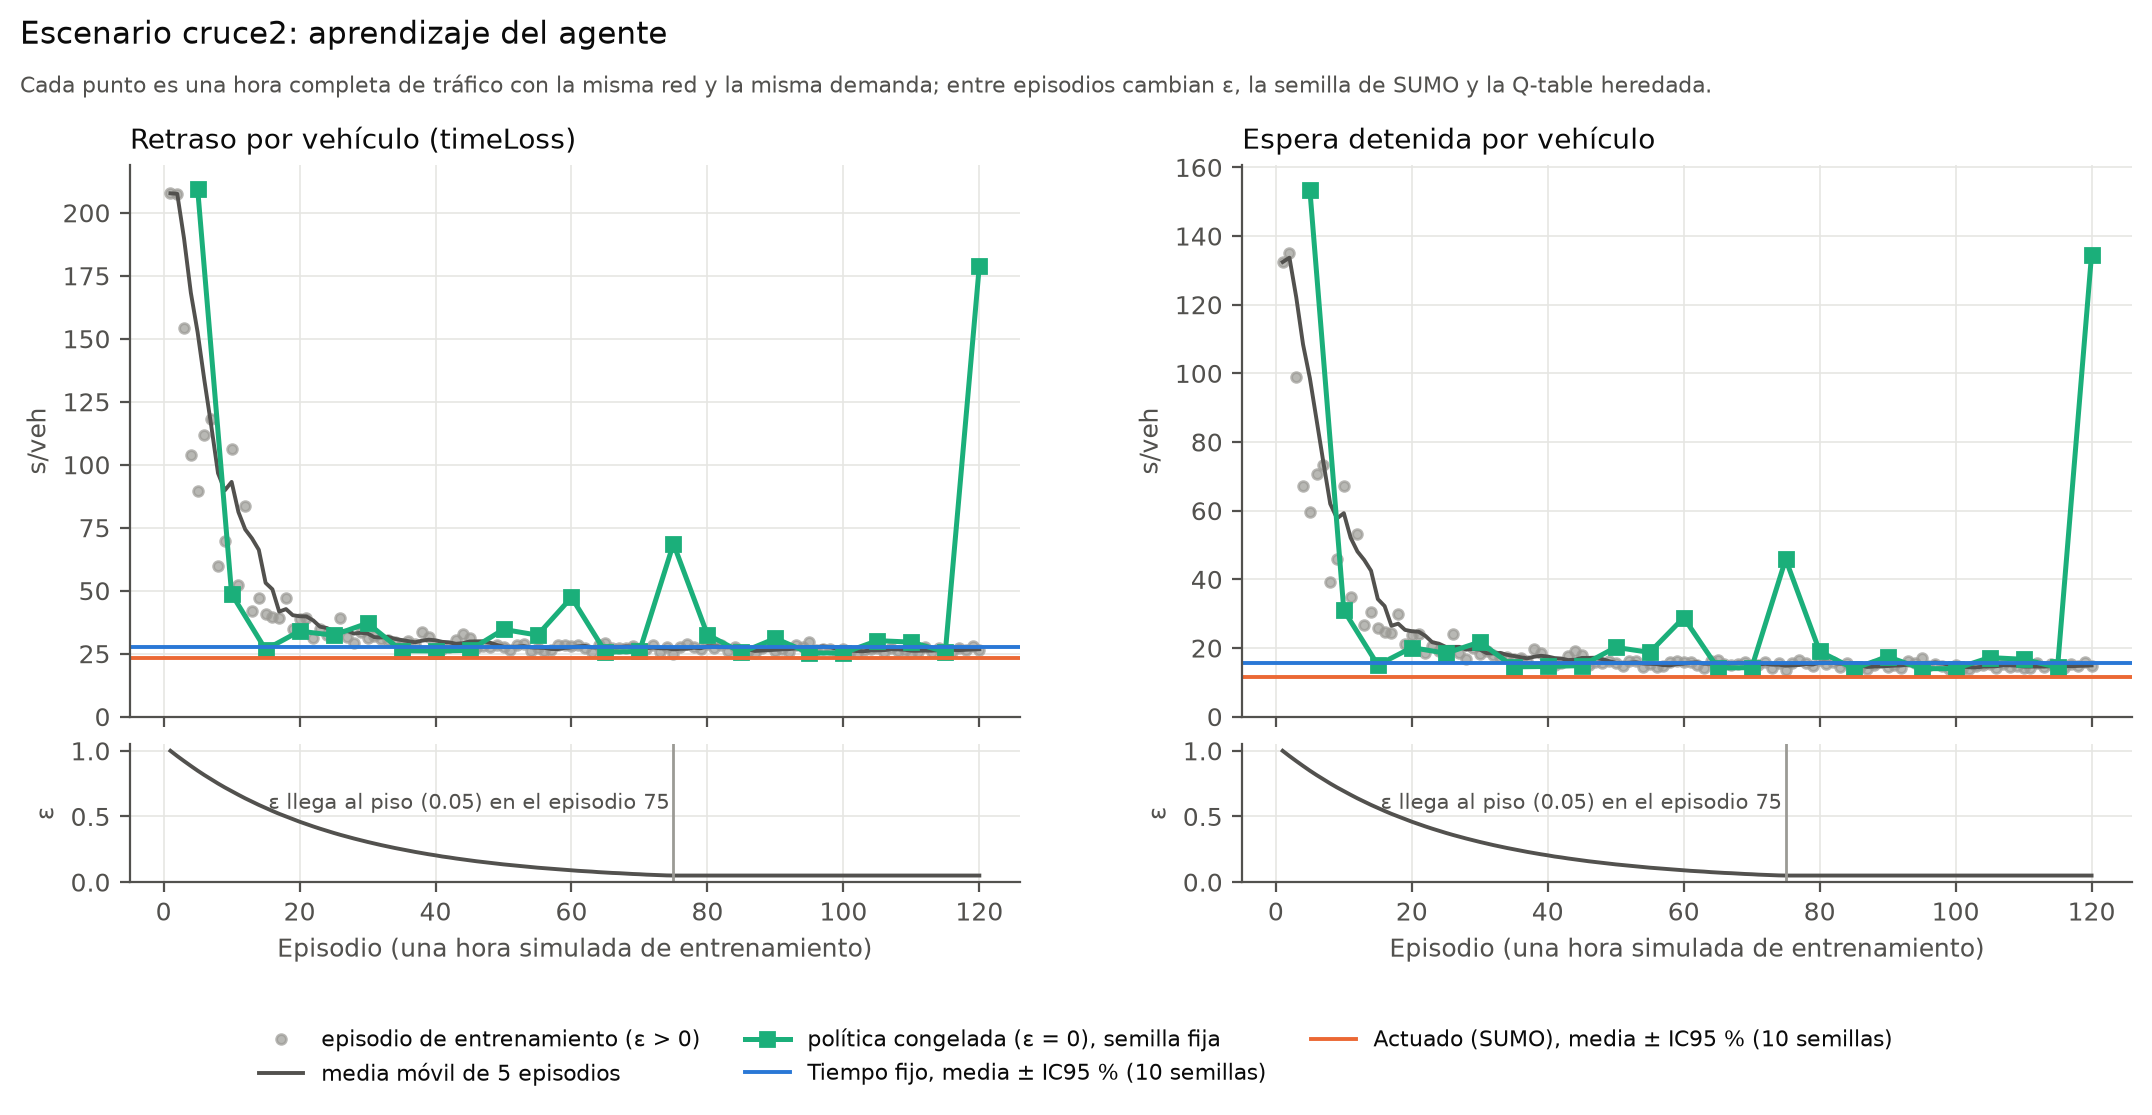
\includegraphics[width=\textwidth]{fig_cruce2_curva.png}
  \caption{Escenario cruce2: aprendizaje del agente con cuatro fases verdes, 120 episodios y decaimiento de $\varepsilon$ de 0.96. Misma convención que la Figura~\ref{fig:cruce-curva}.}
  \label{fig:cruce2-curva}
\end{figure}

\begin{figure}[H]
  \centering
  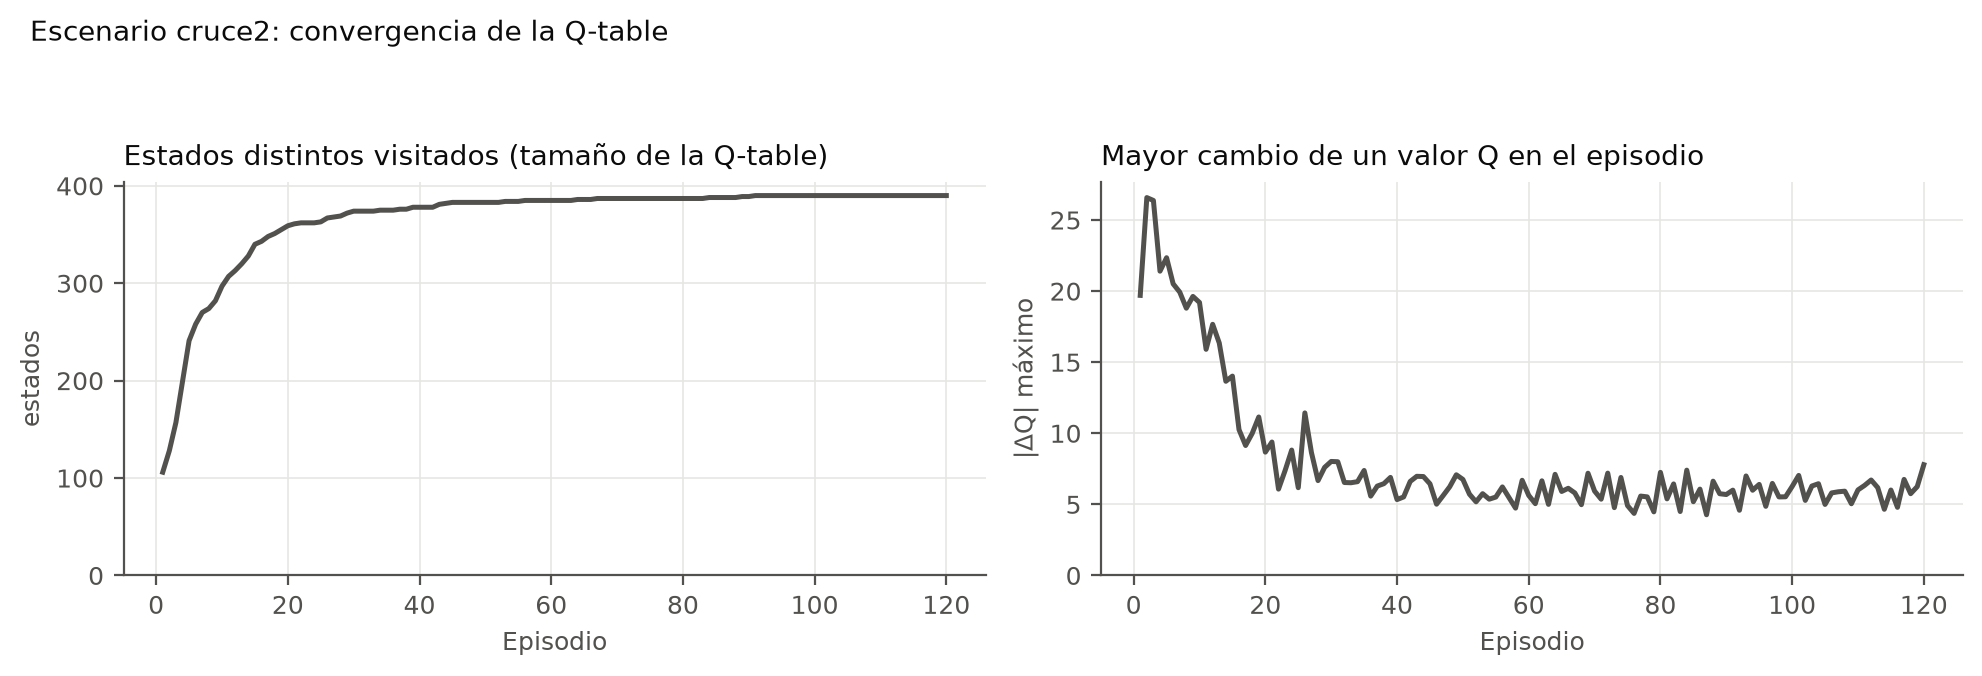
\includegraphics[width=\textwidth]{fig_cruce2_qtable.png}
  \caption{Escenario cruce2: cobertura de la tabla Q (390 de 1024 estados al terminar) y mayor cambio de un valor Q por episodio.}
  \label{fig:cruce2-qtable}
\end{figure}

En la evaluación final (Tabla~\ref{tab:cruce2-evaluacion},
Figura~\ref{fig:cruce2-comparacion}) el agente es peor que el fijo en
todas las métricas: $+17$\,\% de retraso (intervalo $+10$ a $+25$\,\%,
$p = 0.002$), $+18$\,\% de espera, $+23$\,\% de paradas y $+4$\,\% de
CO$_2$, con una desviación estándar del retraso entre semillas unas
diecinueve veces mayor que la del fijo (3.7 frente a 0.2~s). El actuado
reduce el retraso un $16$\,\%. Este es el resultado que
motiva pasar a métodos con aproximación de funciones (DQN, PPO) en el
módulo U2: la representación tabular no cubre el espacio de estados
cuando el semáforo tiene fases de giro protegido, y aumentar los
episodios no lo resuelve, como muestran las evaluaciones intermedias de
la Figura~\ref{fig:cruce2-curva}.

% Generado por tablas_tex.py a partir de los CSV del proyecto. No editar a mano.
\begin{table}[H]
\setstretch{1}
\centering
\scriptsize
\setlength{\tabcolsep}{3pt}
\begin{tabular}{lrrrrrr}
\toprule
Métrica & Tiempo fijo & Actuado & Q-learning & \makecell{$\Delta$ RL vs fijo\\{}[IC95\,\%]} & $p$ & \makecell{$\Delta$ actuado\\vs fijo} \\
\midrule
Retraso (s/veh) & 27.54 $\pm$ 0.14 & 23.21 $\pm$ 0.15 & 32.15 $\pm$ 2.63 & +16.7\,\% [9.9, 25.4] & 0.00195 & $-$15.7\,\% \\
Espera detenida (s/veh) & 15.63 $\pm$ 0.12 & 11.69 $\pm$ 0.14 & 18.51 $\pm$ 1.77 & +18.4\,\% [10.2, 28.7] & 0.00195 & $-$25.2\,\% \\
Cola promedio (veh) & 7.49 $\pm$ 0.07 & 5.75 $\pm$ 0.06 & 9.21 $\pm$ 0.91 & +23.0\,\% [14.3, 34.0] & 0.00195 & $-$23.3\,\% \\
Cola máxima (veh) & 22.50 $\pm$ 0.51 & 17.90 $\pm$ 0.63 & 29.90 $\pm$ 4.31 & +32.9\,\% [19.1, 50.9] & 0.00195 & $-$20.4\,\% \\
Paradas por vehículo & 0.88 $\pm$ 0.01 & 0.84 $\pm$ 0.01 & 1.08 $\pm$ 0.08 & +23.5\,\% [17.5, 31.2] & 0.00195 & $-$4.1\,\% \\
Throughput (veh) & 1840.60 $\pm$ 0.69 & 1844.40 $\pm$ 0.91 & 1842.50 $\pm$ 0.84 & +0.1\,\% [0.0, 0.2] & 0.0156 & +0.2\,\% \\
CO$_2$ (g/veh) & 199.80 $\pm$ 0.26 & 192.91 $\pm$ 0.27 & 207.88 $\pm$ 4.29 & +4.0\,\% [2.5, 6.0] & 0.00195 & $-$3.4\,\% \\
NO$_x$ (mg/veh) & 69.32 $\pm$ 0.09 & 66.64 $\pm$ 0.11 & 72.19 $\pm$ 1.58 & +4.1\,\% [2.5, 6.2] & 0.00195 & $-$3.9\,\% \\
Recompensa por decisión & $-$8.13 $\pm$ 0.07 & $-$6.00 $\pm$ 0.07 & $-$10.04 $\pm$ 1.02 & +23.6\,\% [14.5, 35.1] & 0.00195 & $-$26.2\,\% \\
Cambios de fase & 230.80 $\pm$ 0.74 & 288.30 $\pm$ 2.34 & 280.80 $\pm$ 2.07 & +21.7\,\% [20.9, 22.4] & 0.00195 & +24.9\,\% \\
\bottomrule
\end{tabular}
\caption[Escenario cruce2: evaluación con política congelada]{Escenario cruce2: evaluación con política congelada sobre 10 semillas (1001 a 1010), las mismas para los tres controles. Media $\pm$ IC95\,\%; el cambio porcentual lleva su intervalo bootstrap pareado y $p$ es el de la prueba de Wilcoxon pareada frente al fijo.}
\label{tab:cruce2-evaluacion}
\end{table}


\begin{figure}[H]
  \centering
  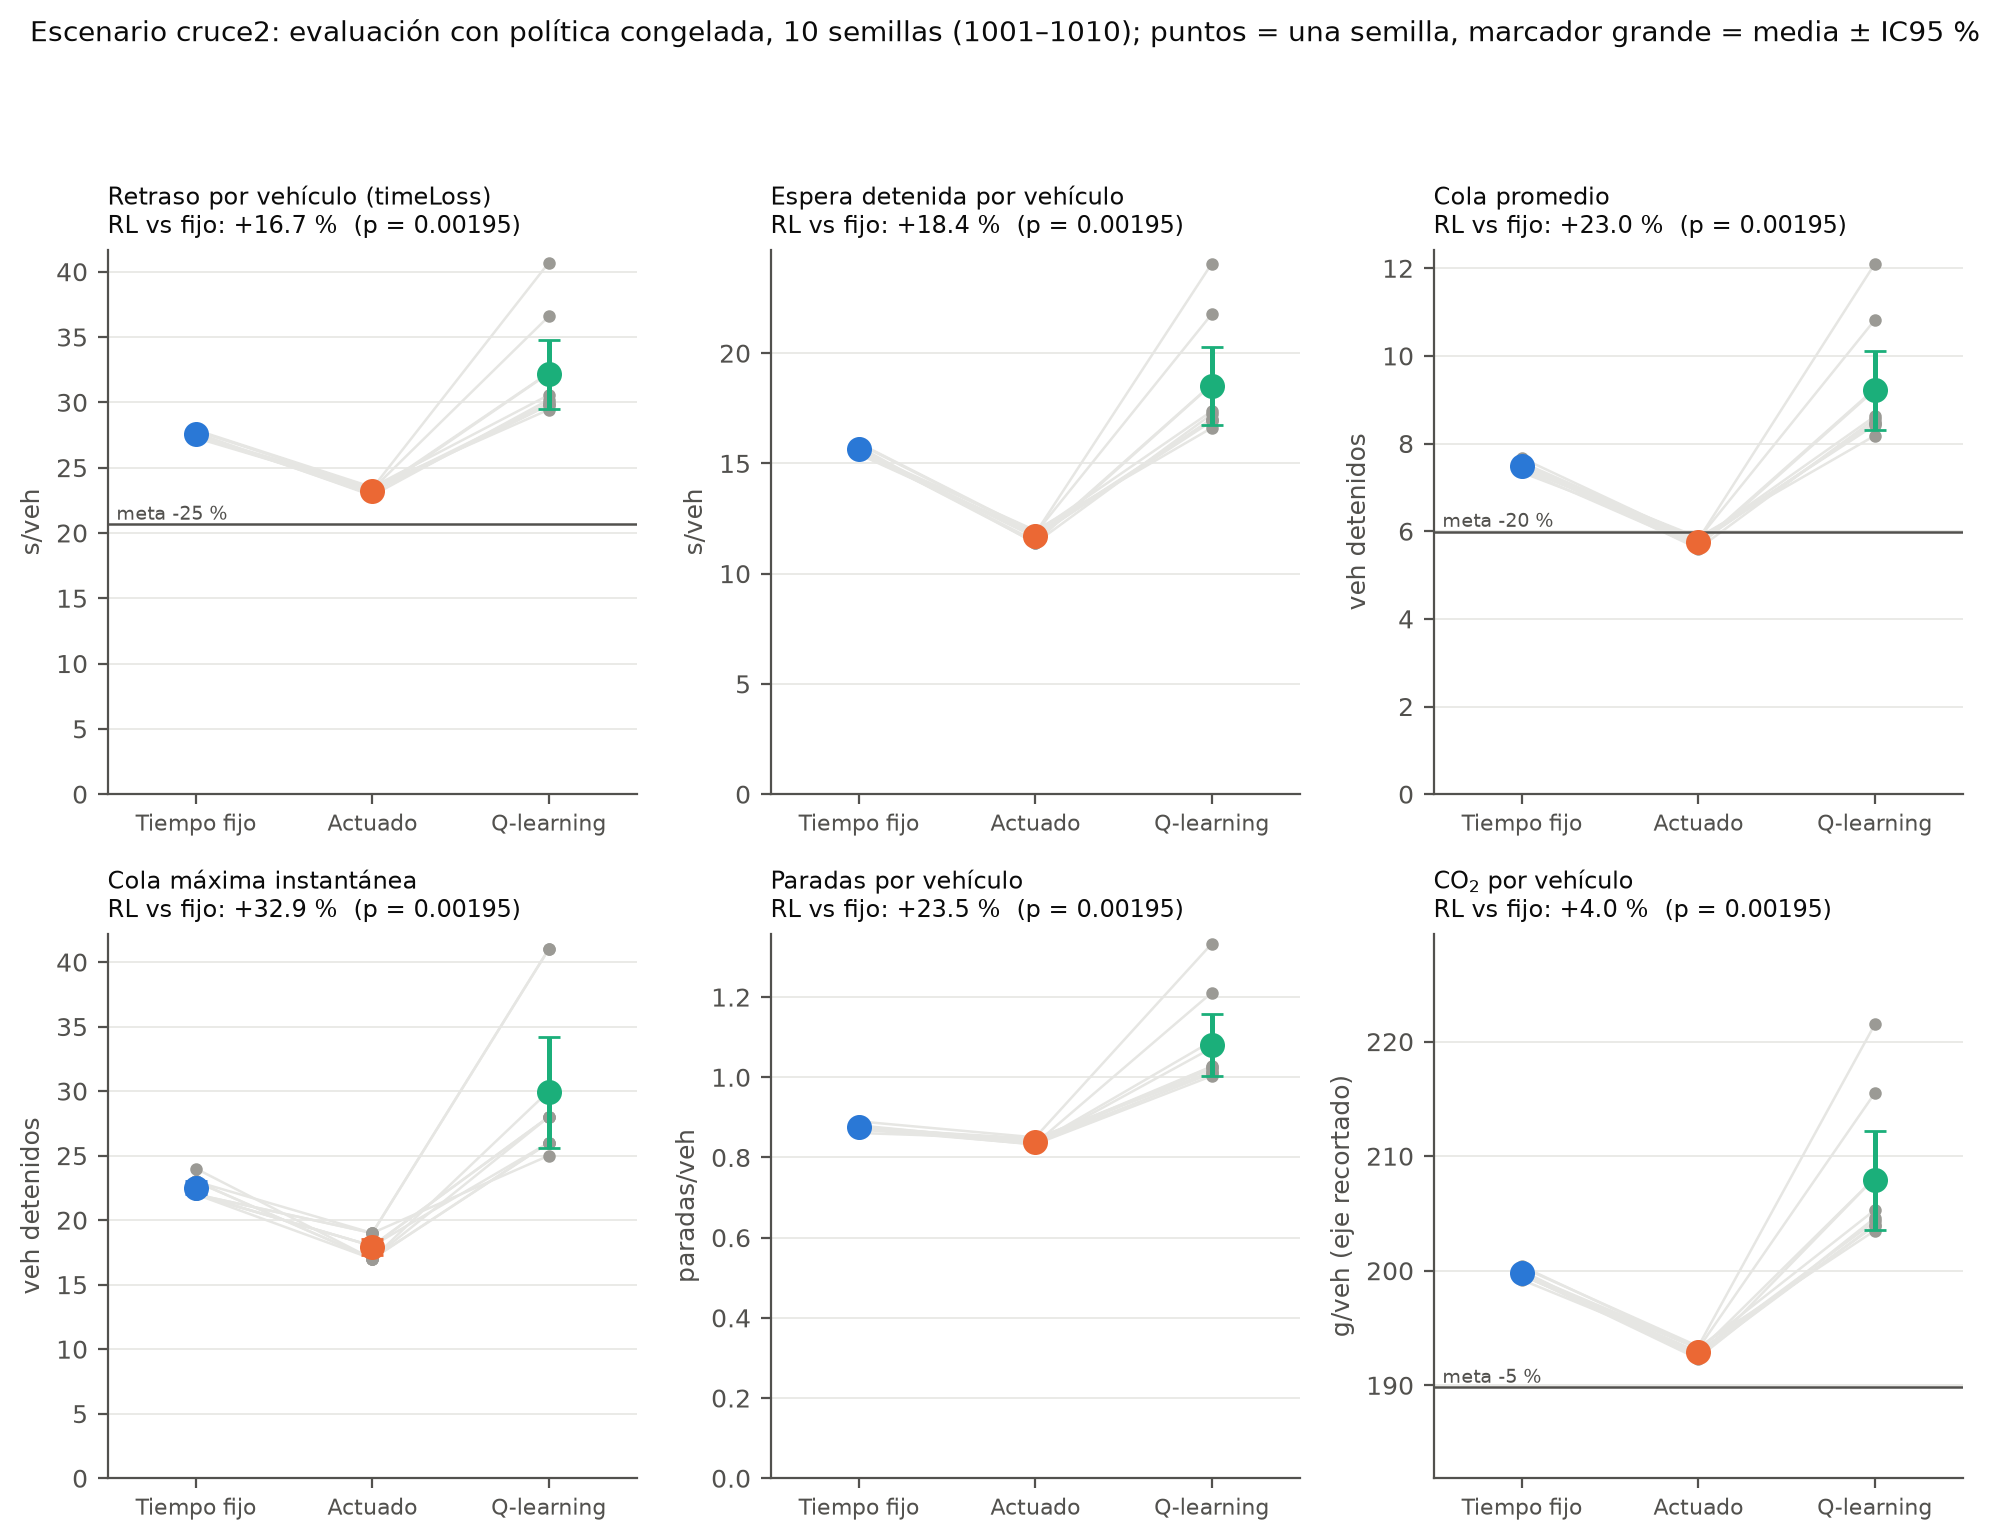
\includegraphics[width=\textwidth]{fig_cruce2_comparacion.png}
  \caption{Escenario cruce2: evaluación con política congelada, diez semillas. Misma convención que la Figura~\ref{fig:cruce-comparacion}.}
  \label{fig:cruce2-comparacion}
\end{figure}

\section{Caso P3: corredor de dos cruces}

En el corredor cada cruce tiene su propio agente, con estado y recompensa
locales y sin comunicación entre ellos. El tiempo fijo de referencia
reparte 20~s a la avenida y 10~s a las transversales, con un desfase de
15~s entre los dos cruces que forma una onda verde en el sentido de la
punta; es el mejor del barrido asimétrico de la
Sección~\ref{sec:escenarios} y da $21.2 \pm 0.4$~s de retraso. Con la
política congelada, los dos agentes quedan muy por detrás de él: el
retraso sube un $60$\,\% (intervalo $+53$ a $+67$\,\%, $p = 0.002$), la
espera detenida un $76$\,\%, la cola promedio un $68$\,\% y las paradas
por vehículo un $94$\,\%, con 463 cambios de fase por hora frente a
410 del fijo; el CO$_2$ sube un $11$\,\%
(Tablas~\ref{tab:corredor-episodios-resumen}
y~\ref{tab:corredor-evaluacion},
Figuras~\ref{fig:corredor-curva} y~\ref{fig:corredor-comparacion}).
Frente al fijo simétrico de 25/25 con desfase de 25~s que se usó en la
primera ronda de ajuste, y que da 31.9~s, la misma política perdía
solo un $6$\,\% y reducía la espera un $13$\,\%: la magnitud de la
derrota del agente depende de lo bien tuneada que esté la referencia,
y por eso se reporta contra la mejor disponible. La evaluación
intermedia oscila entre 24 y 30~s de retraso de una evaluación a la
siguiente, señal de una política inestable. Una corrida previa de este
mismo caso, en la que un desfase del reloj de decisión dejaba el verde
mínimo efectivo en 12~s en vez de 10, había producido una política de
25.8~s en la evaluación final; con la restricción corregida el agente
cambia de fase con más frecuencia y la política resultante da 33.9~s.
Que dos entrenamientos casi idénticos difieran en 8~s, veinte veces el
intervalo de confianza de cualquiera de los dos, muestra la fragilidad
de la política tabular con dos agentes y su sensibilidad al verde
mínimo. El actuado, que tampoco coordina, empata con el fijo tuneado
($-1.1$\,\%, intervalo $-2.5$ a $+0.5$\,\%).

% Generado por tablas_tex.py a partir de los CSV del proyecto. No editar a mano.
\begin{table}[H]
\setstretch{1}
\centering
\scriptsize
\setlength{\tabcolsep}{3pt}
\begin{tabular}{rrrrrrrrrrrr}
\toprule
\multicolumn{4}{c}{Entradas del episodio} & \multicolumn{6}{c}{Salidas del episodio (entrenamiento, $\varepsilon>0$)} & \multicolumn{2}{c}{Política congelada} \\
\cmidrule(lr){1-4}\cmidrule(lr){5-10}\cmidrule(lr){11-12}
Ep. & $\varepsilon$ & Semilla & Q ini. & Retraso & Espera & Cola & $r$/dec. & Cambios & Paradas & Retraso & Espera \\
 &  &  & (estados) & (s/veh) & (s/veh) & (veh) &  & de fase & (/veh) & (s/veh) & (s/veh) \\
\midrule
fijo & 0 & 42 & -- & 31.39 & 14.04 & 7.22 & $-$3.81 & 265 & 1.01 & -- & -- \\
\midrule
1 & 1.000 & 43 & 0 & 86.90 & 38.34 & 17.21 & $-$9.30 & 455 & 3.50 & -- & -- \\
2 & 0.900 & 44 & 133 & 61.99 & 26.70 & 12.51 & $-$6.64 & 450 & 2.60 & -- & -- \\
3 & 0.810 & 45 & 150 & 85.29 & 32.89 & 15.33 & $-$8.12 & 464 & 3.55 & -- & -- \\
5 & 0.656 & 47 & 172 & 34.42 & 13.08 & 6.77 & $-$3.43 & 447 & 1.52 & 24.74 & 8.19 \\
10 & 0.387 & 52 & 188 & 40.19 & 14.72 & 7.48 & $-$3.82 & 456 & 1.78 & 30.09 & 10.90 \\
15 & 0.229 & 57 & 194 & 35.30 & 13.02 & 6.75 & $-$3.40 & 472 & 1.64 & 30.45 & 10.74 \\
20 & 0.135 & 62 & 197 & 29.06 & 10.06 & 5.30 & $-$2.64 & 472 & 1.31 & 23.89 & 7.91 \\
25 & 0.080 & 67 & 201 & 27.95 & 9.90 & 5.28 & $-$2.63 & 441 & 1.22 & 30.14 & 12.26 \\
30 & 0.050 & 72 & 201 & 42.91 & 14.94 & 7.62 & $-$3.87 & 448 & 1.96 & 27.97 & 9.69 \\
35 & 0.050 & 77 & 203 & 28.43 & 9.89 & 5.23 & $-$2.61 & 444 & 1.25 & 24.34 & 7.98 \\
40 & 0.050 & 82 & 204 & 29.29 & 10.60 & 5.59 & $-$2.81 & 448 & 1.27 & 30.14 & 10.81 \\
\bottomrule
\end{tabular}
\caption[Escenario corredor: episodios de entrenamiento]{Escenario corredor: parámetros de entrada y métricas de salida por episodio. 40 episodios de entrenamiento con semilla base 42; la fila fijo es el tiempo fijo con la misma semilla base. La política congelada se evalúa cada 5 episodios con una semilla fija ajena al entrenamiento y a la evaluación final. Se muestran episodios escogidos; la tabla completa está en el Anexo~A.}
\label{tab:corredor-episodios-resumen}
\end{table}



% Generado por tablas_tex.py a partir de los CSV del proyecto. No editar a mano.
\begin{table}[H]
\setstretch{1}
\centering
\scriptsize
\setlength{\tabcolsep}{3pt}
\setlength{\tabcolsep}{2pt}
\begin{tabular}{lrrrrrr}
\toprule
Métrica & Tiempo fijo & Actuado & Q-learning & \makecell{$\Delta$ RL vs fijo\\{}[IC95\,\%]} & $p$ & \makecell{$\Delta$ actuado\\vs fijo} \\
\midrule
Retraso (s/veh) & 21.15 $\pm$ 0.41 & 20.91 $\pm$ 0.25 & 33.86 $\pm$ 1.66 & \makecell{+60.1\,\%\\{}[53.2, 66.9]} & 0.00195 & $-$1.1\,\% \\
Espera detenida (s/veh) & 6.97 $\pm$ 0.18 & 5.90 $\pm$ 0.14 & 12.27 $\pm$ 0.50 & \makecell{+75.9\,\%\\{}[69.4, 82.4]} & 0.00195 & $-$15.4\,\% \\
Cola promedio (veh) & 3.81 $\pm$ 0.08 & 3.32 $\pm$ 0.07 & 6.38 $\pm$ 0.23 & \makecell{+67.5\,\%\\{}[62.5, 72.3]} & 0.00195 & $-$13.0\,\% \\
Cola máxima (veh) & 16.10 $\pm$ 1.52 & 16.70 $\pm$ 1.01 & 22.40 $\pm$ 1.66 & \makecell{+39.1\,\%\\{}[28.0, 53.4]} & 0.00195 & +3.7\,\% \\
Paradas por vehículo & 0.80 $\pm$ 0.02 & 0.83 $\pm$ 0.02 & 1.54 $\pm$ 0.08 & \makecell{+93.6\,\%\\{}[83.8, 103.1]} & 0.00195 & +4.0\,\% \\
Throughput (veh) & 1769.70 $\pm$ 1.43 & 1766.50 $\pm$ 1.27 & 1757.50 $\pm$ 3.85 & \makecell{$-$0.7\,\%\\{}[$-$0.9, $-$0.5]} & 0.00195 & $-$0.2\,\% \\
CO$_2$ (g/veh) & 219.76 $\pm$ 0.82 & 221.59 $\pm$ 0.59 & 244.32 $\pm$ 2.70 & \makecell{+11.2\,\%\\{}[10.1, 12.2]} & 0.00195 & +0.8\,\% \\
NO$_x$ (mg/veh) & 75.59 $\pm$ 0.27 & 75.94 $\pm$ 0.18 & 83.81 $\pm$ 0.92 & \makecell{+10.9\,\%\\{}[9.8, 11.9]} & 0.00195 & +0.5\,\% \\
Recompensa por decisión & $-$1.87 $\pm$ 0.04 & $-$1.58 $\pm$ 0.04 & $-$3.22 $\pm$ 0.12 & \makecell{+72.5\,\%\\{}[67.0, 77.9]} & 0.00195 & $-$15.6\,\% \\
Cambios de fase & 410.40 $\pm$ 0.37 & 459.30 $\pm$ 4.17 & 462.70 $\pm$ 3.04 & \makecell{+12.7\,\%\\{}[12.1, 13.4]} & 0.00195 & +11.9\,\% \\
Viaje extremo a extremo (s) & 105.82 $\pm$ 0.82 & 108.22 $\pm$ 0.50 & 131.81 $\pm$ 2.89 & \makecell{+24.6\,\%\\{}[22.2, 26.9]} & 0.00195 & +2.3\,\% \\
Retraso extremo a extremo (s) & 22.88 $\pm$ 0.77 & 25.27 $\pm$ 0.44 & 48.87 $\pm$ 2.89 & \makecell{+113.6\,\%\\{}[101.4, 125.2]} & 0.00195 & +10.4\,\% \\
Tasa de \textit{spillback} & 0.00 $\pm$ 0.00 & 0.00 $\pm$ 0.00 & 0.00 $\pm$ 0.00 & -- & -- & -- \\
Cola máxima en un enlace (veh) & 7.90 $\pm$ 0.92 & 7.20 $\pm$ 0.45 & 10.90 $\pm$ 1.09 & \makecell{+38.0\,\%\\{}[20.9, 60.6]} & 0.00781 & $-$8.9\,\% \\
\bottomrule
\end{tabular}
\caption[Escenario corredor: evaluación con política congelada]{Escenario corredor: evaluación con política congelada sobre 10 semillas (1001 a 1010), las mismas para los tres controles. Media $\pm$ IC95\,\%; el cambio porcentual lleva su intervalo bootstrap pareado y $p$ es el de la prueba de Wilcoxon pareada frente al fijo.}
\label{tab:corredor-evaluacion}
\end{table}


\begin{figure}[H]
  \centering
  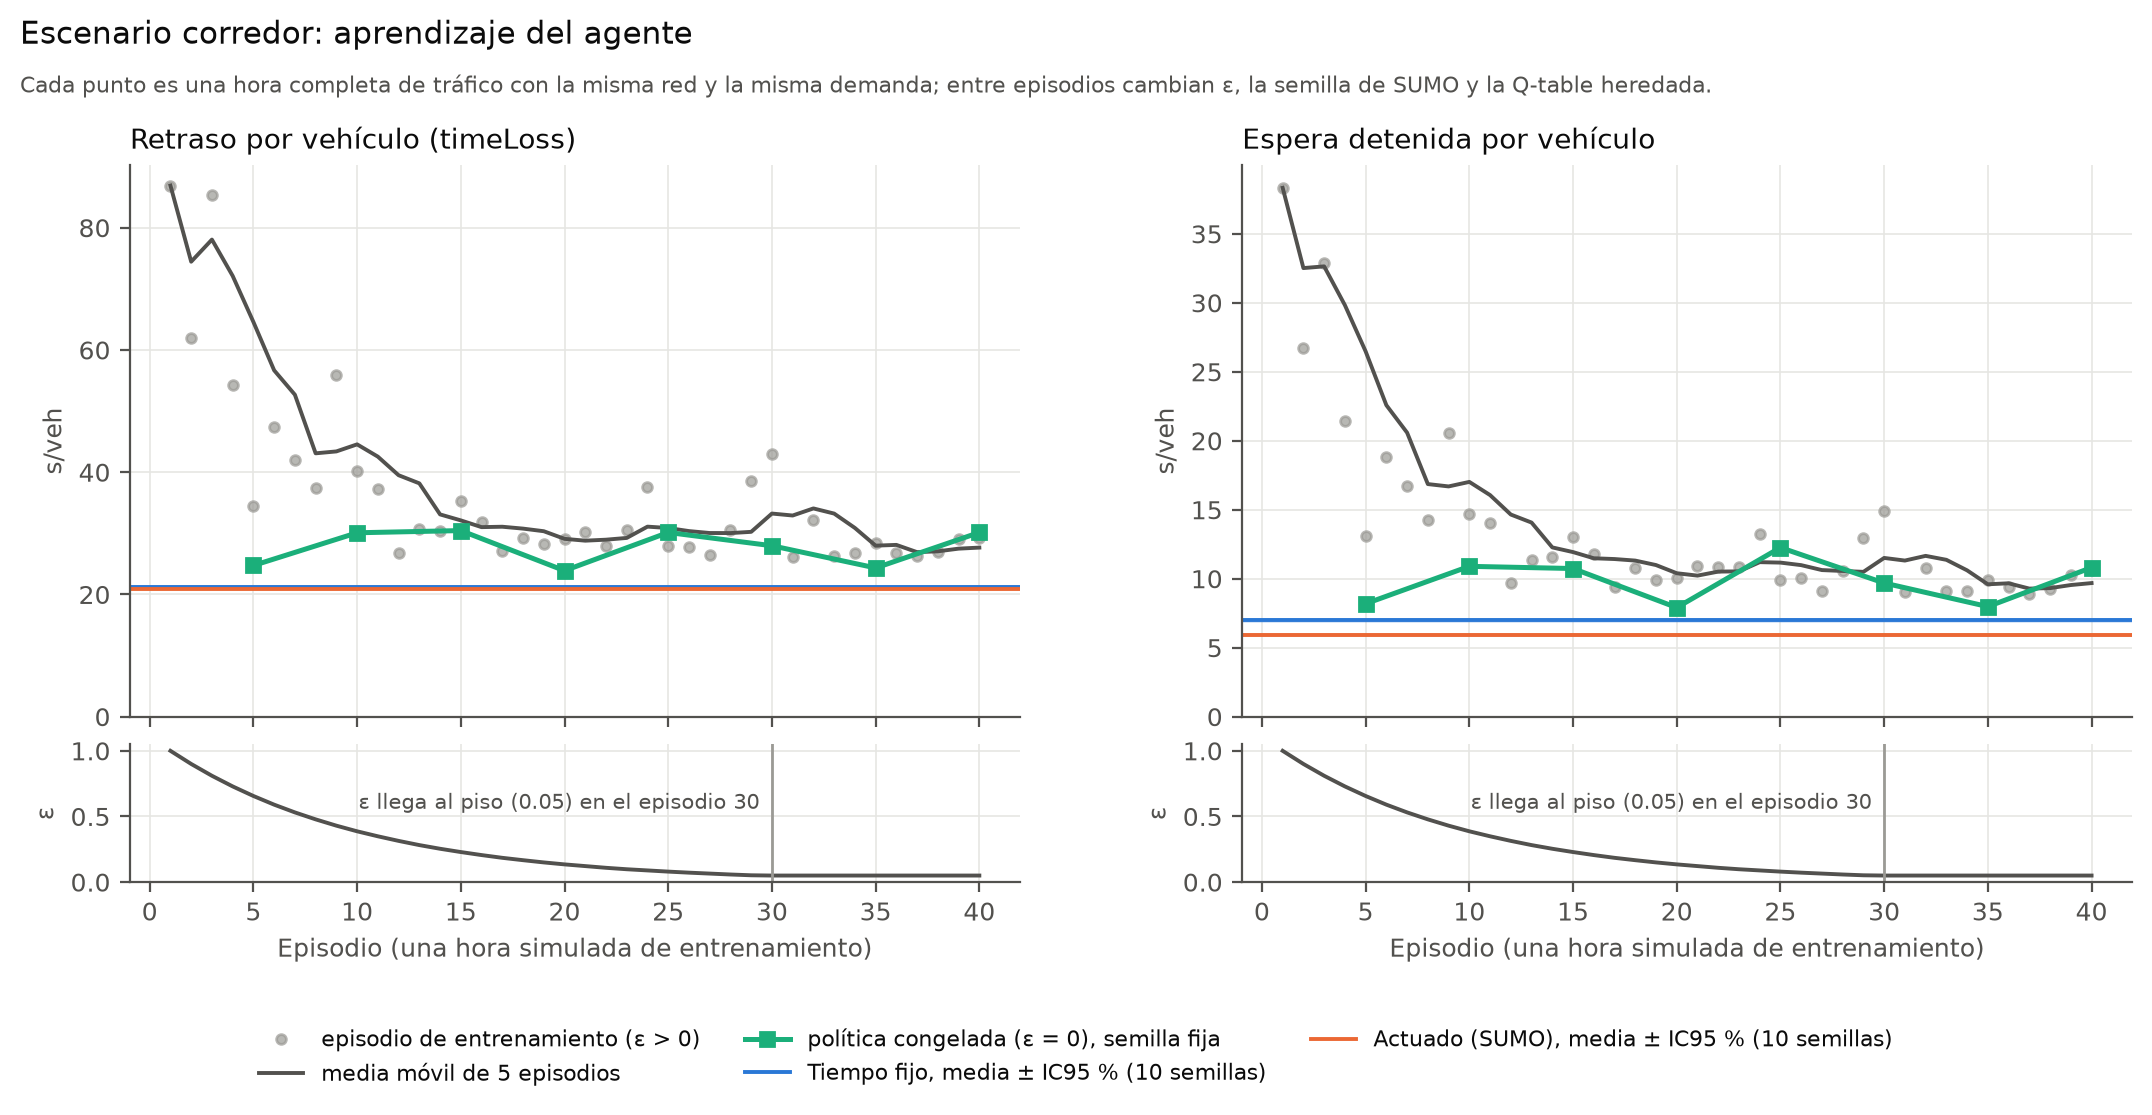
\includegraphics[width=\textwidth]{fig_corredor_curva.png}
  \caption{Escenario corredor: aprendizaje de los dos agentes independientes. Misma convención que la Figura~\ref{fig:cruce-curva}.}
  \label{fig:corredor-curva}
\end{figure}

\begin{figure}[H]
  \centering
  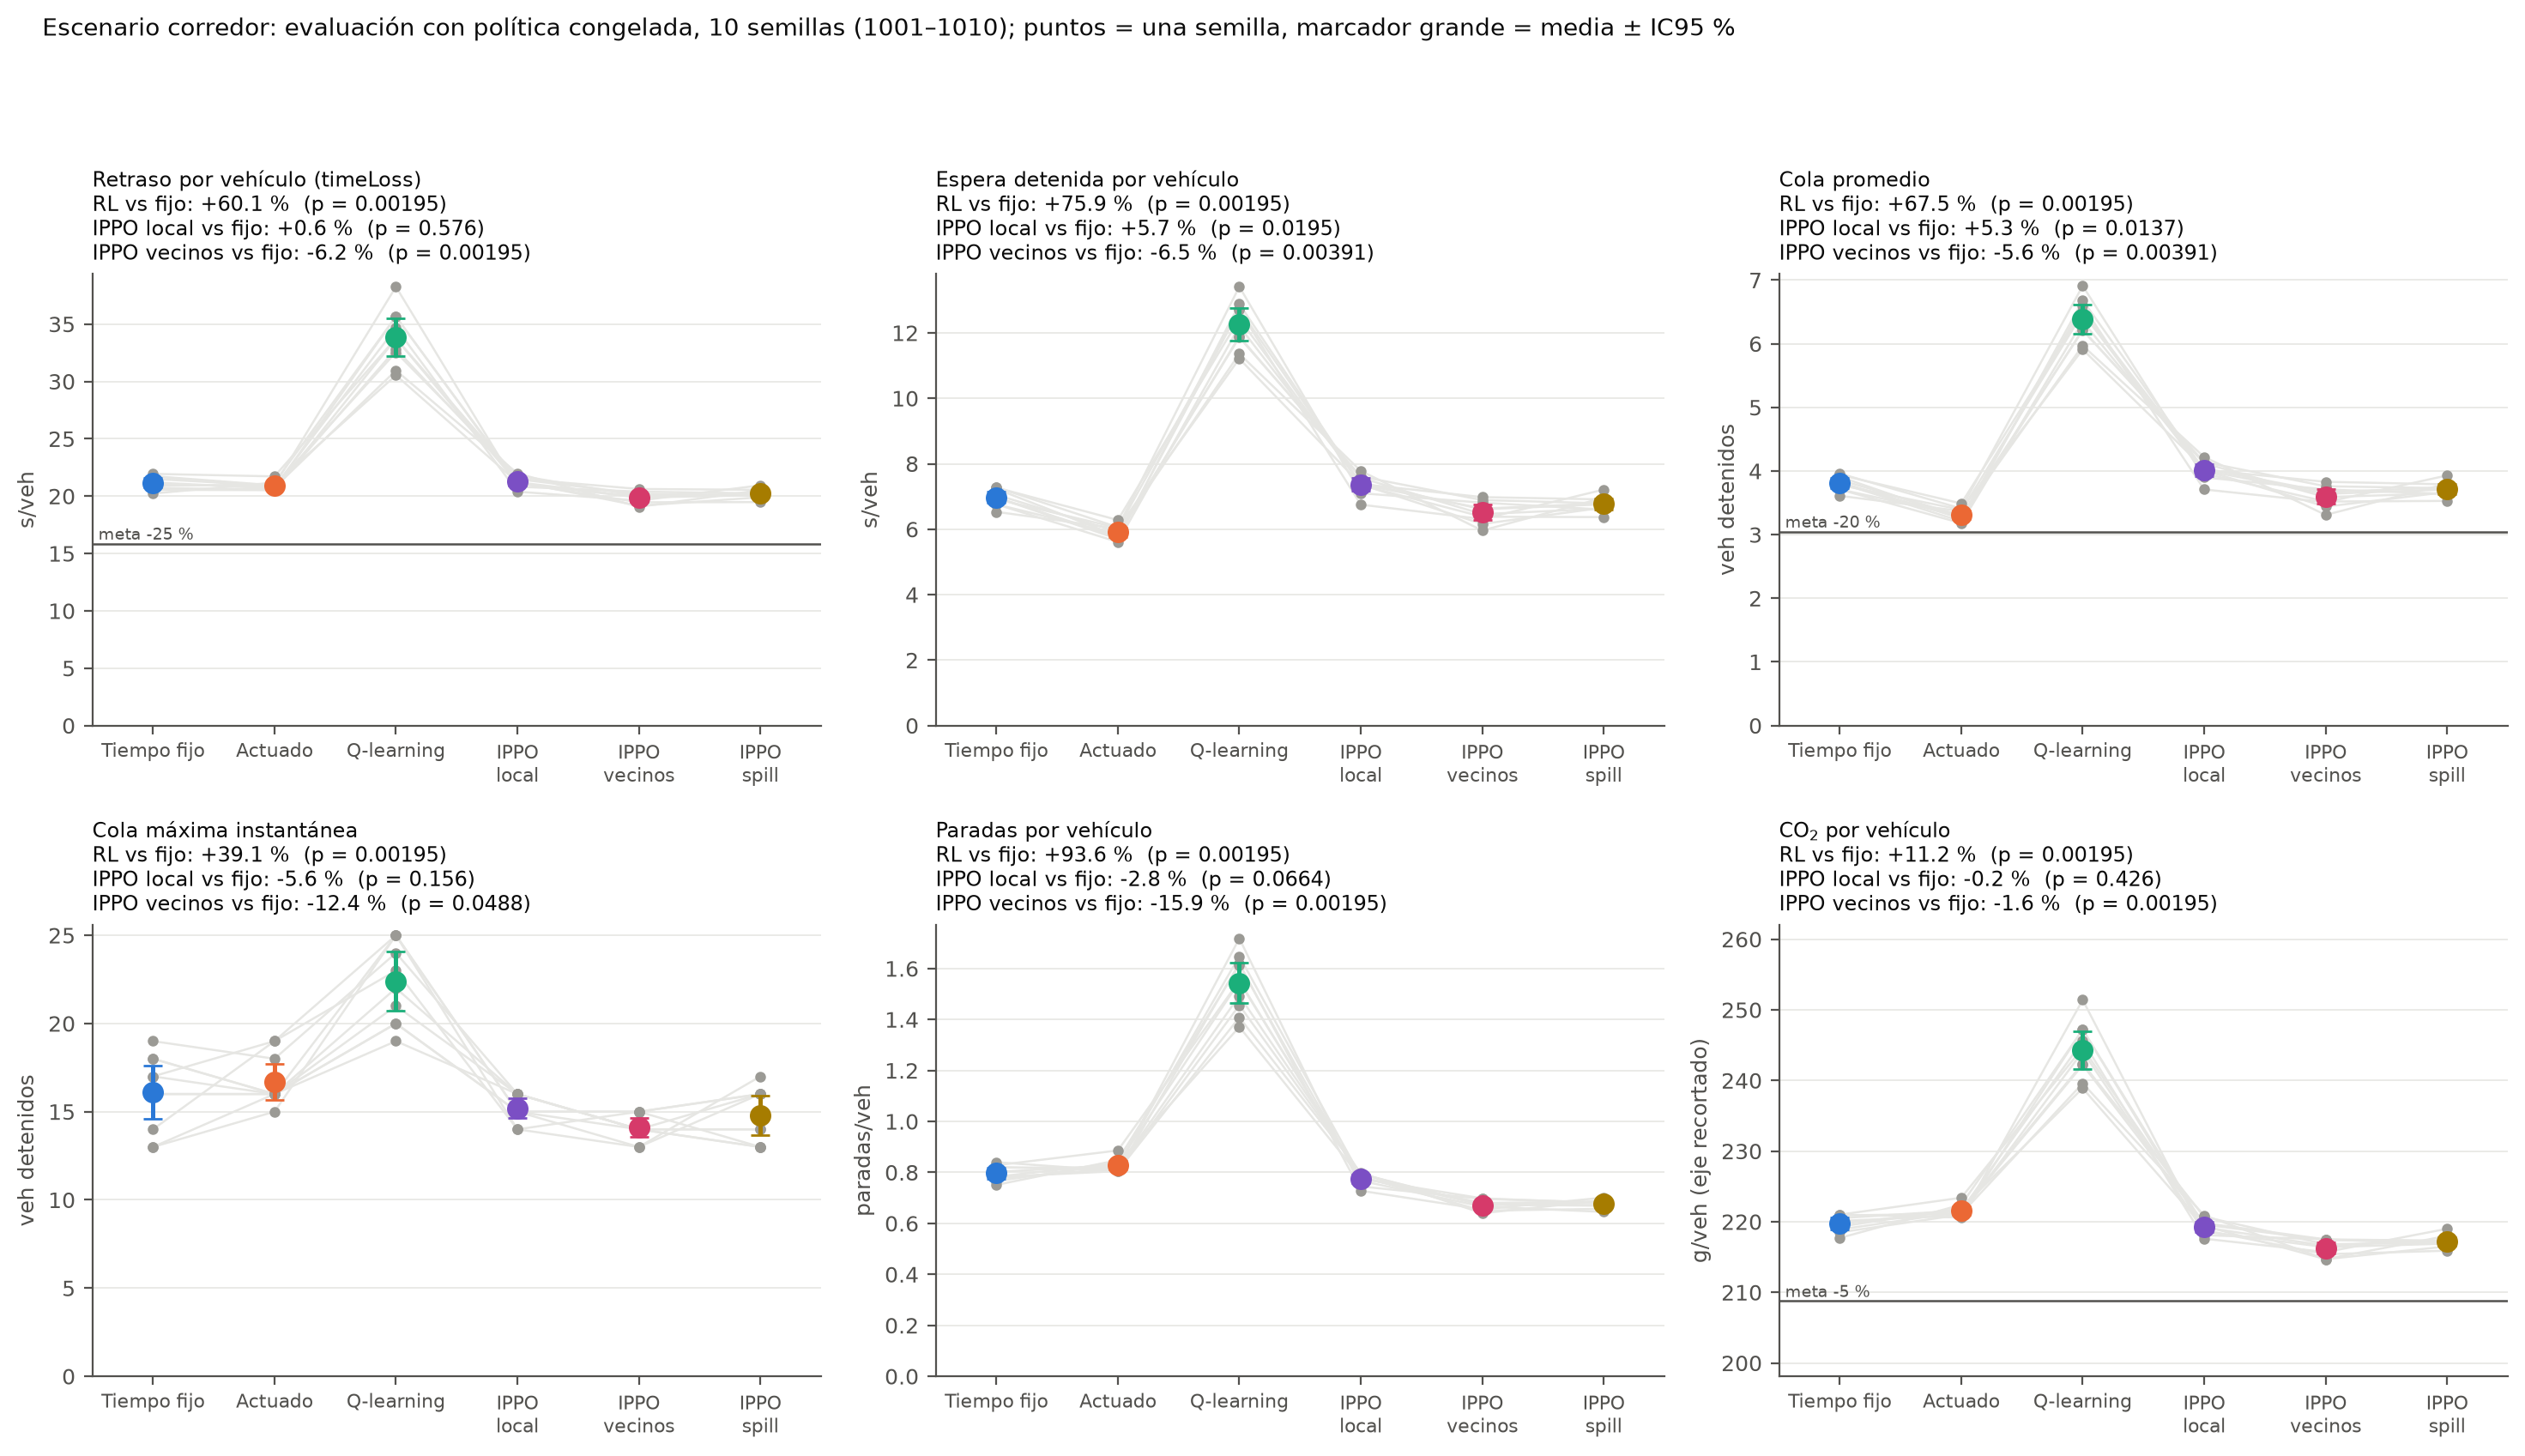
\includegraphics[width=\textwidth]{fig_corredor_comparacion.png}
  \caption{Escenario corredor: evaluación con política congelada, diez semillas. Misma convención que la Figura~\ref{fig:cruce-comparacion}.}
  \label{fig:corredor-comparacion}
\end{figure}

\section{Caso P4: red de tres cruces con onda verde}

En la red, el tiempo fijo de referencia reparte 25~s a la avenida y
15~s a las transversales y coordina los tres cruces con desfases de 0,
23 y 0~s (23~s es el tiempo de viaje entre cruces y el ciclo es de
46~s), de modo que el tercer cruce repite la fase del primero: una onda
verde de tres cruces en el sentido de la punta. Es el mejor del barrido
asimétrico de la Sección~\ref{sec:escenarios} y da $21.8 \pm 0.2$~s de
retraso. Los tres agentes independientes no consiguen igualarla: con la
política congelada el retraso es $15$\,\% mayor que el del fijo
(intervalo $+14$ a $+17$\,\%, $p = 0.002$), la espera $4$\,\% mayor y
las paradas por vehículo suben un $76$\,\%, con $+6$\,\% de CO$_2$
(Tablas~\ref{tab:red-episodios-resumen} y~\ref{tab:red-evaluacion},
Figuras~\ref{fig:red-curva} y~\ref{fig:red-comparacion}). No es falta de
entrenamiento: con 100 episodios y decaimiento 0.95 la evaluación
intermedia se mantiene entre 23.8 y 25.5~s de retraso desde la primera
evaluación (episodio~5) y no muestra tendencia a bajar. Tampoco es que
los agentes sean malos en términos absolutos: el mismo programa fijo sin
desfases entre cruces da $36.4 \pm 0.3$~s de retraso sobre las mismas
diez semillas, muy por encima de los 25.1~s del agente;
lo que los agentes no consiguen es reproducir la progresión de la onda
verde. Cada agente reacciona a su cola local y rompe esa progresión; el
actuado, que tampoco coordina pero reacciona más rápido, apenas mejora
al fijo ($-2$\,\% de retraso) y también aumenta las paradas. Este resultado es la
evidencia empírica que motiva el módulo U4: con varios semáforos
consecutivos, la coordinación anticipada vale más que la reacción local.

% Generado por tablas_tex.py a partir de los CSV del proyecto. No editar a mano.
\begin{table}[H]
\setstretch{1}
\centering
\scriptsize
\setlength{\tabcolsep}{3pt}
\begin{tabular}{rrrrrrrrrrrr}
\toprule
\multicolumn{4}{c}{Entradas del episodio} & \multicolumn{6}{c}{Salidas del episodio (entrenamiento, $\varepsilon>0$)} & \multicolumn{2}{c}{Política congelada} \\
\cmidrule(lr){1-4}\cmidrule(lr){5-10}\cmidrule(lr){11-12}
Ep. & $\varepsilon$ & Semilla & Q ini. & Retraso & Espera & Cola & $r$/dec. & Cambios & Paradas & Retraso & Espera \\
 &  &  & (estados) & (s/veh) & (s/veh) & (veh) &  & de fase & (/veh) & (s/veh) & (s/veh) \\
\midrule
fijo & 0 & 42 & -- & 22.23 & 7.35 & 4.03 & $-$1.43 & 489 & 0.60 & -- & -- \\
\midrule
1 & 1.000 & 43 & 0 & 30.94 & 12.28 & 6.73 & $-$2.41 & 629 & 1.15 & -- & -- \\
2 & 0.950 & 44 & 88 & 30.71 & 12.15 & 6.70 & $-$2.40 & 649 & 1.16 & -- & -- \\
3 & 0.902 & 45 & 108 & 30.71 & 12.23 & 6.70 & $-$2.40 & 637 & 1.14 & -- & -- \\
5 & 0.815 & 47 & 128 & 29.32 & 10.97 & 6.14 & $-$2.18 & 660 & 1.13 & 25.47 & 8.07 \\
10 & 0.630 & 52 & 139 & 27.96 & 10.06 & 5.47 & $-$1.92 & 683 & 1.08 & 25.32 & 8.08 \\
15 & 0.488 & 57 & 140 & 27.57 & 9.68 & 5.30 & $-$1.87 & 708 & 1.11 & 24.88 & 7.67 \\
20 & 0.377 & 62 & 142 & 25.58 & 8.38 & 4.47 & $-$1.56 & 737 & 1.04 & 24.78 & 7.93 \\
25 & 0.292 & 67 & 143 & 26.52 & 8.95 & 4.92 & $-$1.71 & 724 & 1.09 & 24.29 & 7.19 \\
30 & 0.226 & 72 & 144 & 25.91 & 8.69 & 4.47 & $-$1.54 & 736 & 1.08 & 24.27 & 7.31 \\
35 & 0.175 & 77 & 145 & 24.72 & 7.72 & 4.26 & $-$1.49 & 707 & 1.00 & 24.44 & 7.65 \\
40 & 0.135 & 82 & 145 & 24.41 & 7.54 & 4.17 & $-$1.45 & 733 & 0.97 & 23.91 & 7.29 \\
45 & 0.105 & 87 & 145 & 25.28 & 8.08 & 4.27 & $-$1.48 & 769 & 1.06 & 25.49 & 7.90 \\
50 & 0.081 & 92 & 145 & 24.85 & 7.80 & 4.35 & $-$1.50 & 746 & 1.03 & 24.00 & 7.03 \\
55 & 0.063 & 97 & 145 & 24.73 & 7.73 & 4.20 & $-$1.45 & 768 & 1.01 & 24.72 & 7.71 \\
60 & 0.050 & 102 & 145 & 25.00 & 7.89 & 4.38 & $-$1.52 & 757 & 1.03 & 24.45 & 7.69 \\
65 & 0.050 & 107 & 146 & 25.31 & 8.04 & 4.36 & $-$1.50 & 761 & 1.03 & 24.36 & 7.51 \\
70 & 0.050 & 112 & 146 & 24.45 & 7.56 & 4.22 & $-$1.46 & 748 & 0.97 & 24.23 & 7.40 \\
75 & 0.050 & 117 & 148 & 24.86 & 7.74 & 4.25 & $-$1.47 & 750 & 1.02 & 23.85 & 7.15 \\
80 & 0.050 & 122 & 148 & 24.52 & 7.57 & 4.26 & $-$1.47 & 747 & 0.97 & 23.77 & 7.03 \\
85 & 0.050 & 127 & 148 & 24.59 & 7.73 & 4.25 & $-$1.47 & 748 & 1.00 & 24.46 & 7.56 \\
90 & 0.050 & 132 & 149 & 24.63 & 7.69 & 4.22 & $-$1.47 & 766 & 0.99 & 24.38 & 7.56 \\
95 & 0.050 & 137 & 149 & 24.30 & 7.65 & 4.11 & $-$1.43 & 758 & 0.95 & 24.85 & 7.73 \\
100 & 0.050 & 142 & 149 & 25.36 & 8.16 & 4.58 & $-$1.59 & 761 & 1.05 & 24.84 & 7.58 \\
\bottomrule
\end{tabular}
\caption[Escenario red: episodios de entrenamiento]{Escenario red: parámetros de entrada y métricas de salida por episodio. 100 episodios de entrenamiento con semilla base 42; la fila fijo es el tiempo fijo con la misma semilla base. La política congelada se evalúa cada 5 episodios con una semilla fija ajena al entrenamiento y a la evaluación final. Se muestran episodios escogidos; la tabla completa está en el Anexo~A.}
\label{tab:red-episodios-resumen}
\end{table}



% Generado por tablas_tex.py a partir de los CSV del proyecto. No editar a mano.
\begin{table}[H]
\setstretch{1}
\centering
\scriptsize
\setlength{\tabcolsep}{3pt}
\setlength{\tabcolsep}{2pt}
\begin{tabular}{lrrrrrr}
\toprule
Métrica & Tiempo fijo & Actuado & Q-learning & \makecell{$\Delta$ RL vs fijo\\{}[IC95\,\%]} & $p$ & \makecell{$\Delta$ actuado\\vs fijo} \\
\midrule
Retraso (s/veh) & 21.78 $\pm$ 0.22 & 21.42 $\pm$ 0.23 & 25.12 $\pm$ 0.31 & \makecell{+15.3\,\%\\{}[13.9, 16.8]} & 0.00195 & $-$1.7\,\% \\
Espera detenida (s/veh) & 7.41 $\pm$ 0.16 & 5.45 $\pm$ 0.19 & 7.71 $\pm$ 0.15 & \makecell{+4.0\,\%\\{}[1.4, 6.6]} & 0.0195 & $-$26.5\,\% \\
Cola promedio (veh) & 4.01 $\pm$ 0.05 & 2.93 $\pm$ 0.08 & 4.26 $\pm$ 0.11 & \makecell{+6.2\,\%\\{}[3.7, 8.8]} & 0.00391 & $-$27.1\,\% \\
Cola máxima (veh) & 14.90 $\pm$ 0.63 & 15.70 $\pm$ 1.22 & 18.20 $\pm$ 0.94 & \makecell{+22.1\,\%\\{}[15.7, 28.7]} & 0.00195 & +5.4\,\% \\
Paradas por vehículo & 0.61 $\pm$ 0.01 & 0.80 $\pm$ 0.01 & 1.07 $\pm$ 0.02 & \makecell{+75.6\,\%\\{}[72.5, 78.7]} & 0.00195 & +31.5\,\% \\
Throughput (veh) & 2095.10 $\pm$ 1.14 & 2093.00 $\pm$ 1.65 & 2090.80 $\pm$ 1.81 & \makecell{$-$0.2\,\%\\{}[$-$0.3, $-$0.1]} & 0.00391 & $-$0.1\,\% \\
CO$_2$ (g/veh) & 250.39 $\pm$ 0.47 & 256.56 $\pm$ 0.57 & 265.09 $\pm$ 0.73 & \makecell{+5.9\,\%\\{}[5.6, 6.2]} & 0.00195 & +2.5\,\% \\
NO$_x$ (mg/veh) & 86.46 $\pm$ 0.15 & 87.93 $\pm$ 0.18 & 90.81 $\pm$ 0.21 & \makecell{+5.0\,\%\\{}[4.8, 5.3]} & 0.00195 & +1.7\,\% \\
Recompensa por decisión & $-$1.43 $\pm$ 0.02 & $-$1.01 $\pm$ 0.03 & $-$1.47 $\pm$ 0.04 & \makecell{+2.9\,\%\\{}[0.3, 5.6]} & 0.084 & $-$29.6\,\% \\
Cambios de fase & 489.60 $\pm$ 0.91 & 784.00 $\pm$ 4.12 & 763.30 $\pm$ 3.04 & \makecell{+55.9\,\%\\{}[55.4, 56.4]} & 0.00195 & +60.1\,\% \\
Viaje extremo a extremo (s) & 155.37 $\pm$ 0.46 & 160.66 $\pm$ 0.39 & 166.52 $\pm$ 0.96 & \makecell{+7.2\,\%\\{}[6.8, 7.6]} & 0.00195 & +3.4\,\% \\
Retraso extremo a extremo (s) & 23.45 $\pm$ 0.31 & 28.75 $\pm$ 0.36 & 34.59 $\pm$ 0.80 & \makecell{+47.5\,\%\\{}[45.0, 50.4]} & 0.00195 & +22.6\,\% \\
Tasa de \textit{spillback} & 0.00 $\pm$ 0.00 & 0.00 $\pm$ 0.00 & 0.00 $\pm$ 0.00 & -- & -- & -- \\
Cola máxima en un enlace (veh) & 1.90 $\pm$ 0.23 & 4.40 $\pm$ 0.37 & 4.80 $\pm$ 0.30 & \makecell{+152.6\,\%\\{}[130.0, 188.2]} & 0.00195 & +131.6\,\% \\
\bottomrule
\end{tabular}
\caption[Escenario red: evaluación con política congelada]{Escenario red: evaluación con política congelada sobre 10 semillas (1001 a 1010), las mismas para los tres controles. Media $\pm$ IC95\,\%; el cambio porcentual lleva su intervalo bootstrap pareado y $p$ es el de la prueba de Wilcoxon pareada frente al fijo.}
\label{tab:red-evaluacion}
\end{table}


\begin{figure}[H]
  \centering
  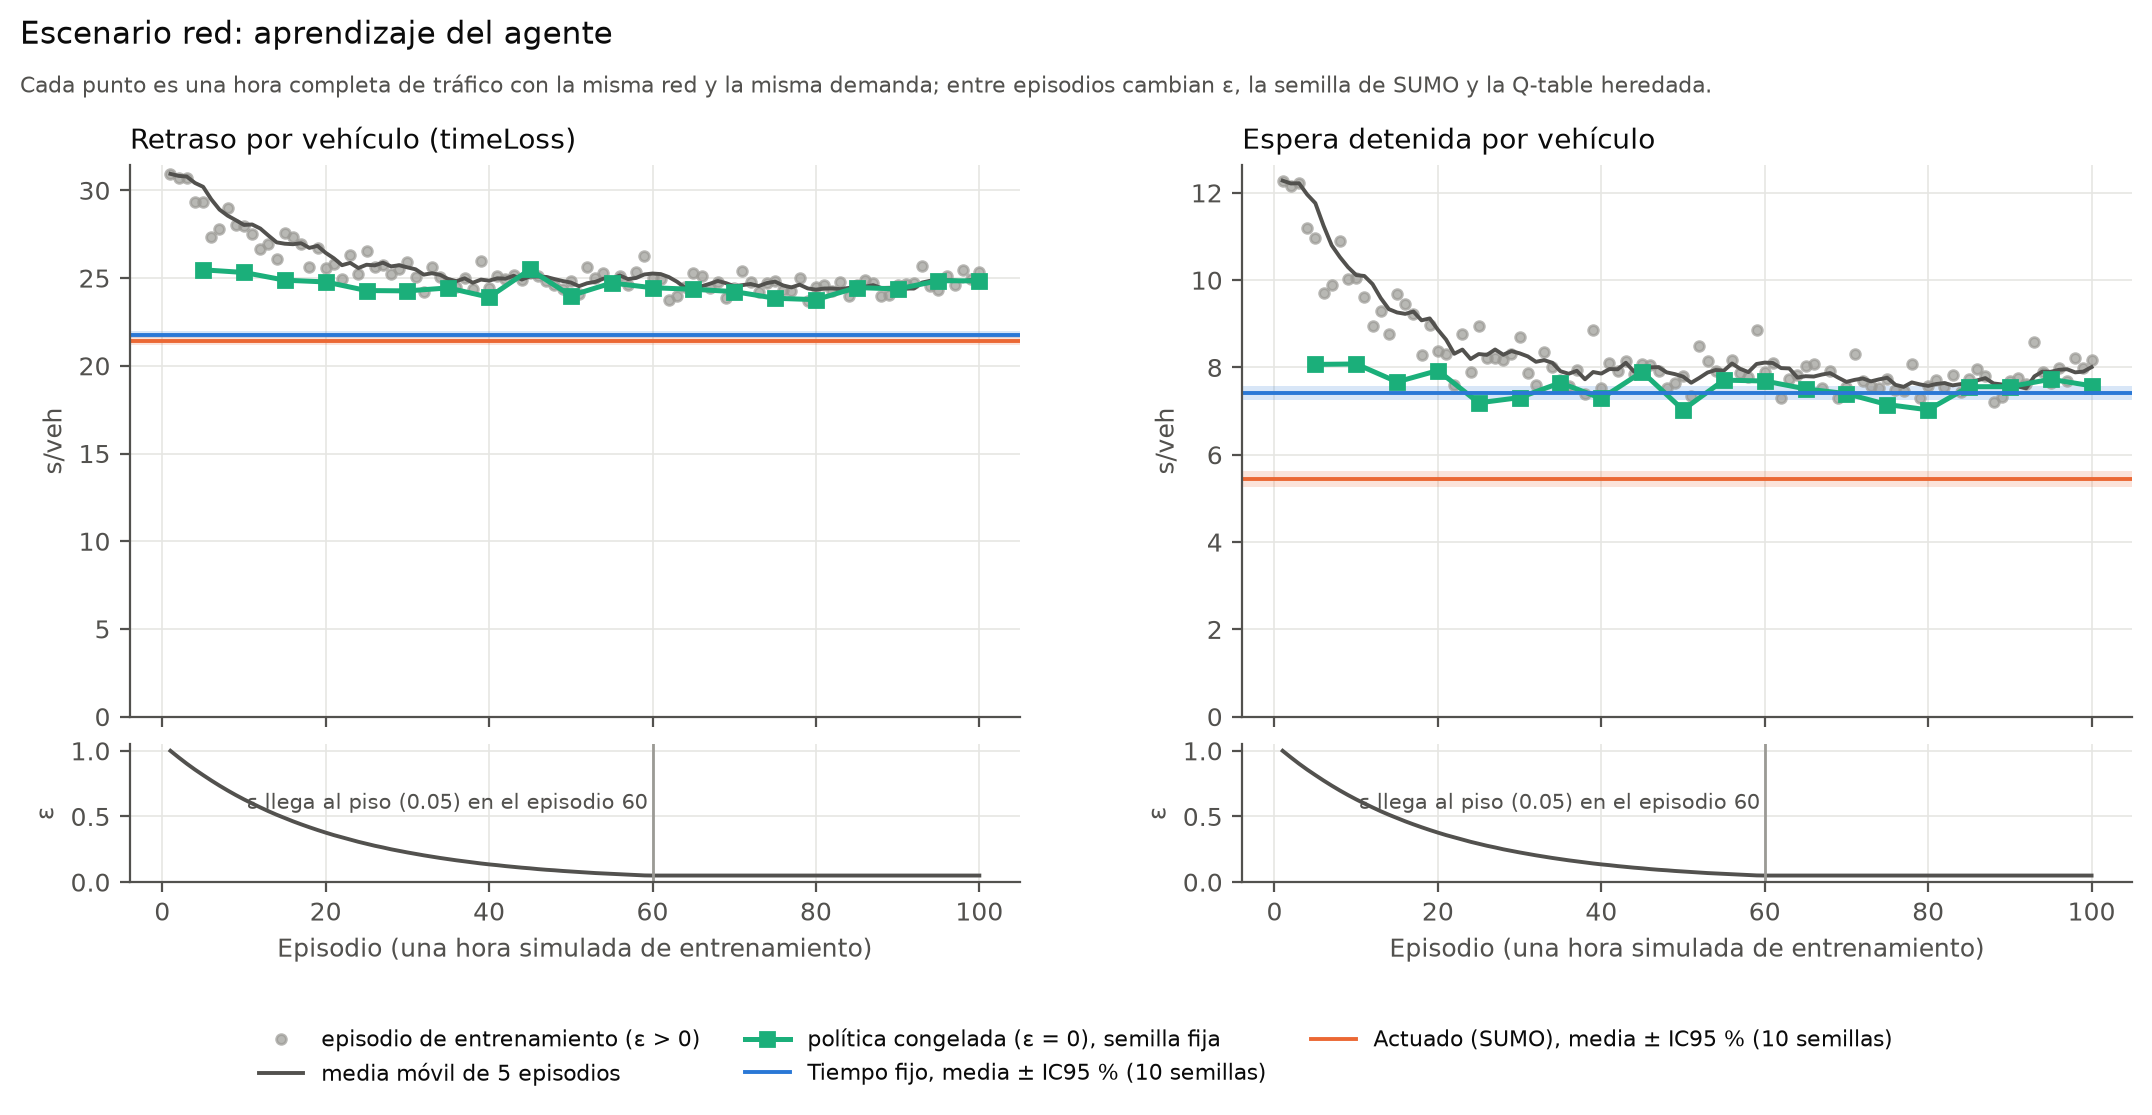
\includegraphics[width=\textwidth]{fig_red_curva.png}
  \caption{Escenario red: aprendizaje de los tres agentes independientes, 100 episodios y decaimiento de $\varepsilon$ de 0.95. Misma convención que la Figura~\ref{fig:cruce-curva}.}
  \label{fig:red-curva}
\end{figure}

\begin{figure}[H]
  \centering
  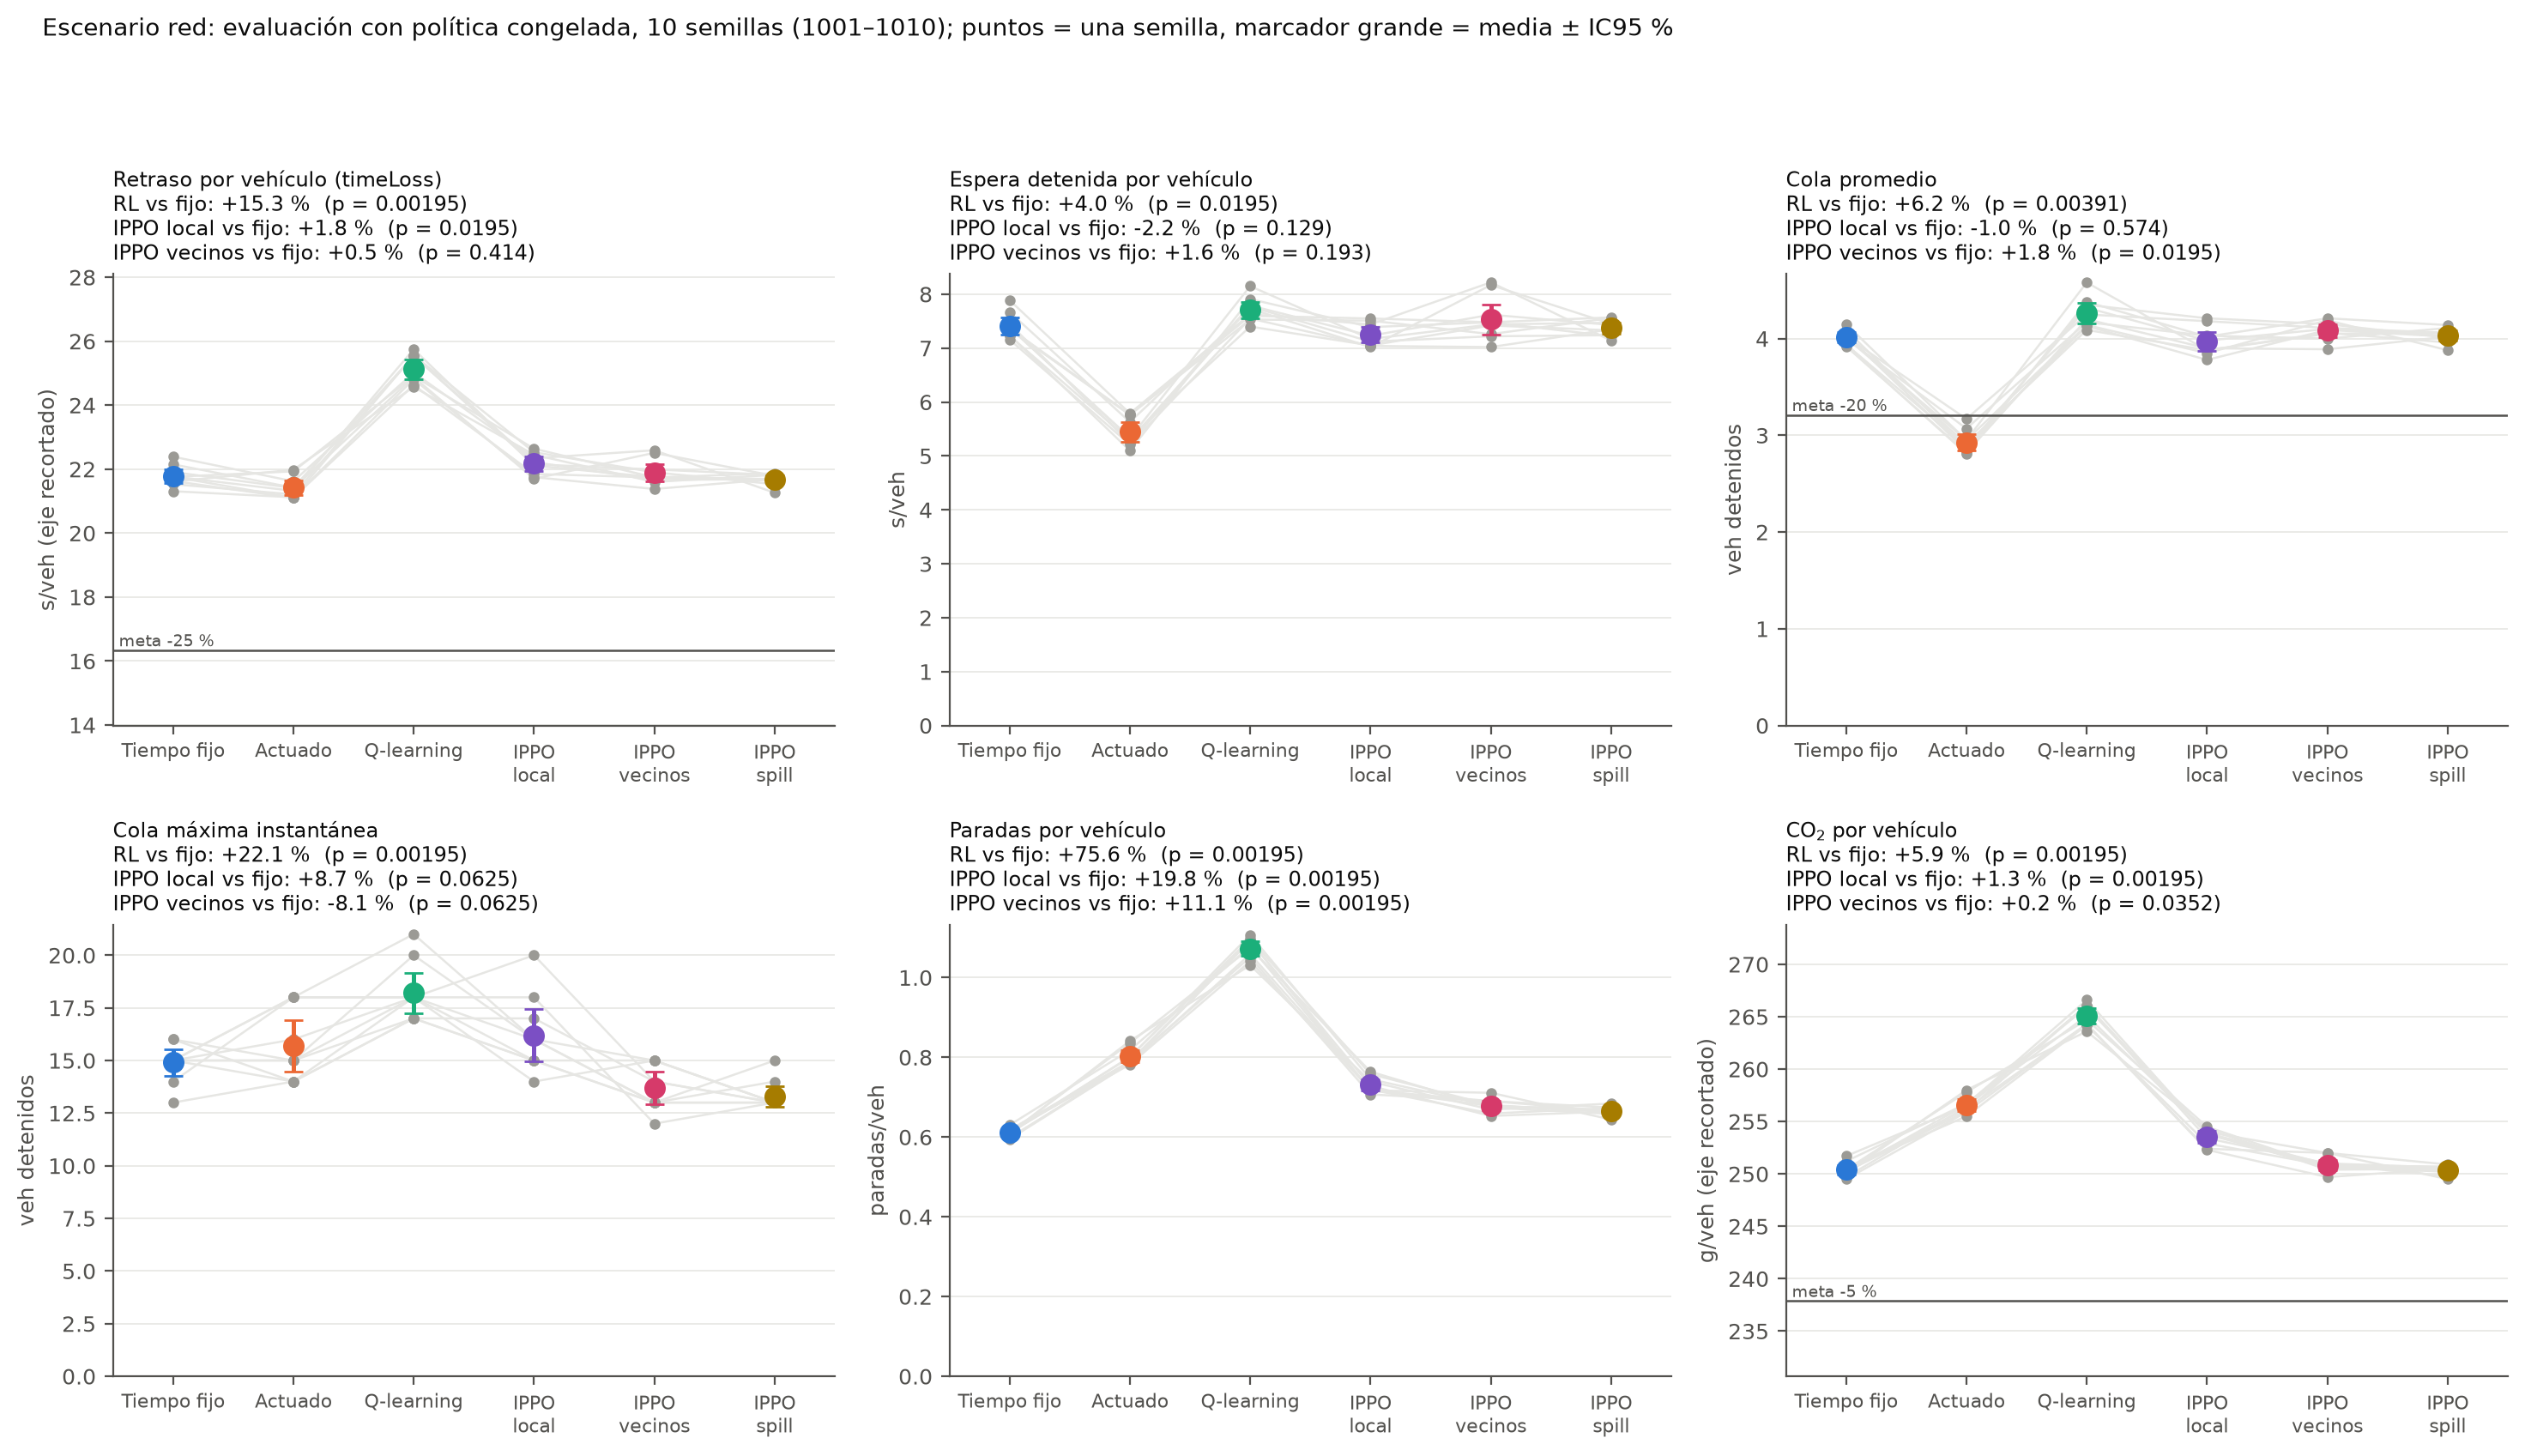
\includegraphics[width=\textwidth]{fig_red_comparacion.png}
  \caption{Escenario red: evaluación con política congelada, diez semillas. Misma convención que la Figura~\ref{fig:cruce-comparacion}.}
  \label{fig:red-comparacion}
\end{figure}

\section{Módulo U4: coordinación con IPPO}
\label{sec:resultados-u4}

Los resultados de esta sección siguen el plan de pruebas del módulo U4
(Sección~\ref{sec:plan}): los mismos controles de referencia y las
mismas diez semillas de evaluación, más las variantes IPPO de la
Sección~\ref{sec:u4}, cada una representada por la política mediana de
sus tres semillas base. La Tabla~\ref{tab:resumen-u4} adelanta la
métrica primaria de los escenarios de varios cruces; el nivel de éxito
alcanzado, según el criterio prefijado, se resume al final.

% Generado por tablas_tex.py a partir de los CSV del proyecto. No editar a mano.
\begin{table}[H]
\setstretch{1}
\centering
\scriptsize
\setlength{\tabcolsep}{3pt}
\begin{tabular}{lrrrrrrrrr}
\toprule
 & \multicolumn{6}{c}{Retraso (s/veh)} & \multicolumn{2}{c}{IPPO vecinos vs fijo} & \makecell{IPPO vecinos\\vs actuado} \\
\cmidrule(lr){2-7}\cmidrule(lr){8-9}
Escenario & Fijo & Actuado & Q-learning & \makecell{IPPO\\local} & \makecell{IPPO\\vecinos} & \makecell{IPPO\\spill} & $\Delta$ [IC95\,\%] & $p$ & $\Delta$ [IC95\,\%] \\
\midrule
corredor & 21.15 & 20.91 & 33.86 & 21.27 & 19.84 & 20.21 & \makecell{$-$6.2\,\%\\{}[$-$8.0, $-$4.6]} & 0.00195 & \makecell{$-$5.1\,\%\\{}[$-$6.4, $-$3.9]} \\
red & 21.78 & 21.42 & 25.12 & 22.17 & 21.89 & 21.68 & \makecell{+0.5\,\%\\{}[$-$0.3, 1.3]} & 0.414 & \makecell{+2.2\,\%\\{}[0.8, 3.5]} \\
corredor\_alta & 153.88 & 122.97 & 211.12 & 121.97 & 121.33 & 122.78 & \makecell{$-$21.2\,\%\\{}[$-$22.2, $-$20.0]} & 0.00195 & \makecell{$-$1.3\,\%\\{}[$-$3.8, 1.4]} \\
\bottomrule
\end{tabular}
\caption[Resumen del módulo U4]{Resumen del módulo U4: retraso promedio por vehículo con política congelada sobre las semillas de evaluación, comunes a todos los brazos. Cada variante IPPO es su política mediana.}
\label{tab:resumen-u4}
\end{table}


\subsection*{Prueba de humo: cruce de dos fases}

La compuerta de entrada del módulo (variante \emph{local}, un solo
semáforo, 60 episodios) resultó ser, además, el primer resultado que
alcanza la meta de la tesis. Con la política congelada y las diez
semillas del protocolo, IPPO local reduce el retraso un $35$\,\% frente
al fijo (intervalo $-36$ a $-34$\,\%, $p = 0.002$), un $31$\,\% frente
al agente Q-learning del mismo cruce y un $2.6$\,\% frente al actuado
(intervalo $-3.2$ a $-2.0$\,\%), al que ningún control aprendido había
igualado hasta aquí (Tablas~\ref{tab:cruce-u4}
y~\ref{tab:cruce-u4-deltas}, Figura~\ref{fig:cruce-curva-ippo}). Lo
consigue con un $17$\,\% más de cambios de fase que el fijo, no un
$77$\,\% como el tabular, y con menos paradas por vehículo que
cualquiera de los tres controles ($-39$\,\% frente al fijo); la cola
media baja a la mitad y el CO$_2$ un $9$\,\%, con lo que las metas de
colas ($-20$\,\%) y emisiones ($-5$\,\%) también se cumplen en este
caso. La evaluación intermedia iguala al actuado desde el episodio 20 y
termina en 14.9~s; las dos corridas de ajuste de la
Sección~\ref{sec:u4} que ya usaban el presupuesto de optimización
definitivo, con semillas base 43 y 45, terminan en 14.8 y 14.7~s (la
tercera, que solo bajaba $\gamma$, quedó en 19.9~s). Con los
hiperparámetros finales, en el cruce aislado el resultado no depende de
la semilla de entrenamiento. Dos precisiones
acotan la lectura. Es un solo semáforo, donde la coordinación no
interviene, y la comparación con Q-learning es de paquete completo:
cambian el estado (continuo, con vehículos en movimiento y tiempo de
verde), la recompensa (retraso en lugar de cola detenida) y el
algoritmo.

% Generado por tablas_tex.py a partir de los CSV del proyecto. No editar a mano.
\begin{table}[H]
\setstretch{1}
\centering
\scriptsize
\setlength{\tabcolsep}{3pt}
\begin{tabular}{p{3.3cm}rrrr}
\toprule
Métrica & \makecell{Fijo} & \makecell{Actuado} & \makecell{Q-learning} & \makecell{IPPO\\local} \\
\midrule
Retraso (s/veh) & 23.19 $\pm$ 0.25 & 15.46 $\pm$ 0.18 & 21.72 $\pm$ 1.00 & 15.05 $\pm$ 0.21 \\
Espera detenida (s/veh) & 9.63 $\pm$ 0.20 & 3.79 $\pm$ 0.05 & 7.14 $\pm$ 0.49 & 4.32 $\pm$ 0.10 \\
Cola promedio (veh) & 5.31 $\pm$ 0.10 & 2.40 $\pm$ 0.03 & 4.07 $\pm$ 0.23 & 2.67 $\pm$ 0.05 \\
Cola máxima (veh) & 18.00 $\pm$ 0.67 & 11.50 $\pm$ 0.77 & 18.40 $\pm$ 0.69 & 10.50 $\pm$ 0.77 \\
Paradas por vehículo & 0.68 $\pm$ 0.01 & 0.49 $\pm$ 0.01 & 0.87 $\pm$ 0.05 & 0.41 $\pm$ 0.01 \\
Throughput (veh) & 1802 $\pm$ 1 & 1808 $\pm$ 1 & 1803 $\pm$ 3 & 1808 $\pm$ 1 \\
CO$_2$ (g/veh) & 196.11 $\pm$ 0.55 & 180.54 $\pm$ 0.47 & 193.13 $\pm$ 1.84 & 177.77 $\pm$ 0.41 \\
NO$_x$ (mg/veh) & 67.34 $\pm$ 0.19 & 61.72 $\pm$ 0.13 & 65.97 $\pm$ 0.64 & 60.98 $\pm$ 0.13 \\
Recompensa por decisión & $-$5.74 $\pm$ 0.12 & $-$2.48 $\pm$ 0.03 & $-$4.23 $\pm$ 0.26 & $-$2.84 $\pm$ 0.06 \\
Cambios de fase & 131.40 $\pm$ 0.37 & 203.00 $\pm$ 2.02 & 232.70 $\pm$ 3.66 & 153.90 $\pm$ 1.63 \\
\bottomrule
\end{tabular}
\caption[Escenario cruce: evaluación de las variantes IPPO]{Escenario cruce: evaluación con política congelada sobre 10 semillas (1001 a 1010), las mismas para todos los brazos; media $\pm$ IC95\,\%. Cada variante IPPO es la política mediana de sus semillas base por la evaluación intermedia final; los cambios porcentuales están en la Tabla~\ref{tab:cruce-u4-deltas}.}
\label{tab:cruce-u4}
\end{table}
\begin{table}[H]
\setstretch{1}
\centering
\scriptsize
\setlength{\tabcolsep}{3pt}
\begin{tabular}{lrrrrrrr}
\toprule
 & Retraso & \multicolumn{3}{c}{Cambio del retraso [IC95\,\%]} & \multicolumn{3}{c}{vs fijo, secundarias} \\
\cmidrule(lr){3-5}\cmidrule(lr){6-8}
Variante & (s/veh) & vs fijo & vs actuado & vs Q-learning & Espera & Paradas & Cambios \\
\midrule
IPPO local & 15.05 & \makecell[r]{$-$35.1\,\%\\{}[$-$36.0, $-$34.2]\\$p$ = 0.00195} & \makecell[r]{$-$2.6\,\%\\{}[$-$3.2, $-$2.0]\\$p$ = 0.00195} & \makecell[r]{$-$30.7\,\%\\{}[$-$33.0, $-$28.2]\\$p$ = 0.00195} & $-$55.2\,\% & $-$39.3\,\% & +17.1\,\% \\
\bottomrule
\end{tabular}
\caption[Escenario cruce: cambio del retraso de las variantes IPPO]{Escenario cruce: cambio porcentual del retraso de cada variante IPPO (política mediana) frente al fijo, al actuado y a Q-learning, con intervalo bootstrap pareado por semilla y $p$ de Wilcoxon pareado; a la derecha, cambio frente al fijo de tres secundarias.}
\label{tab:cruce-u4-deltas}
\end{table}


\begin{figure}[H]
  \centering
  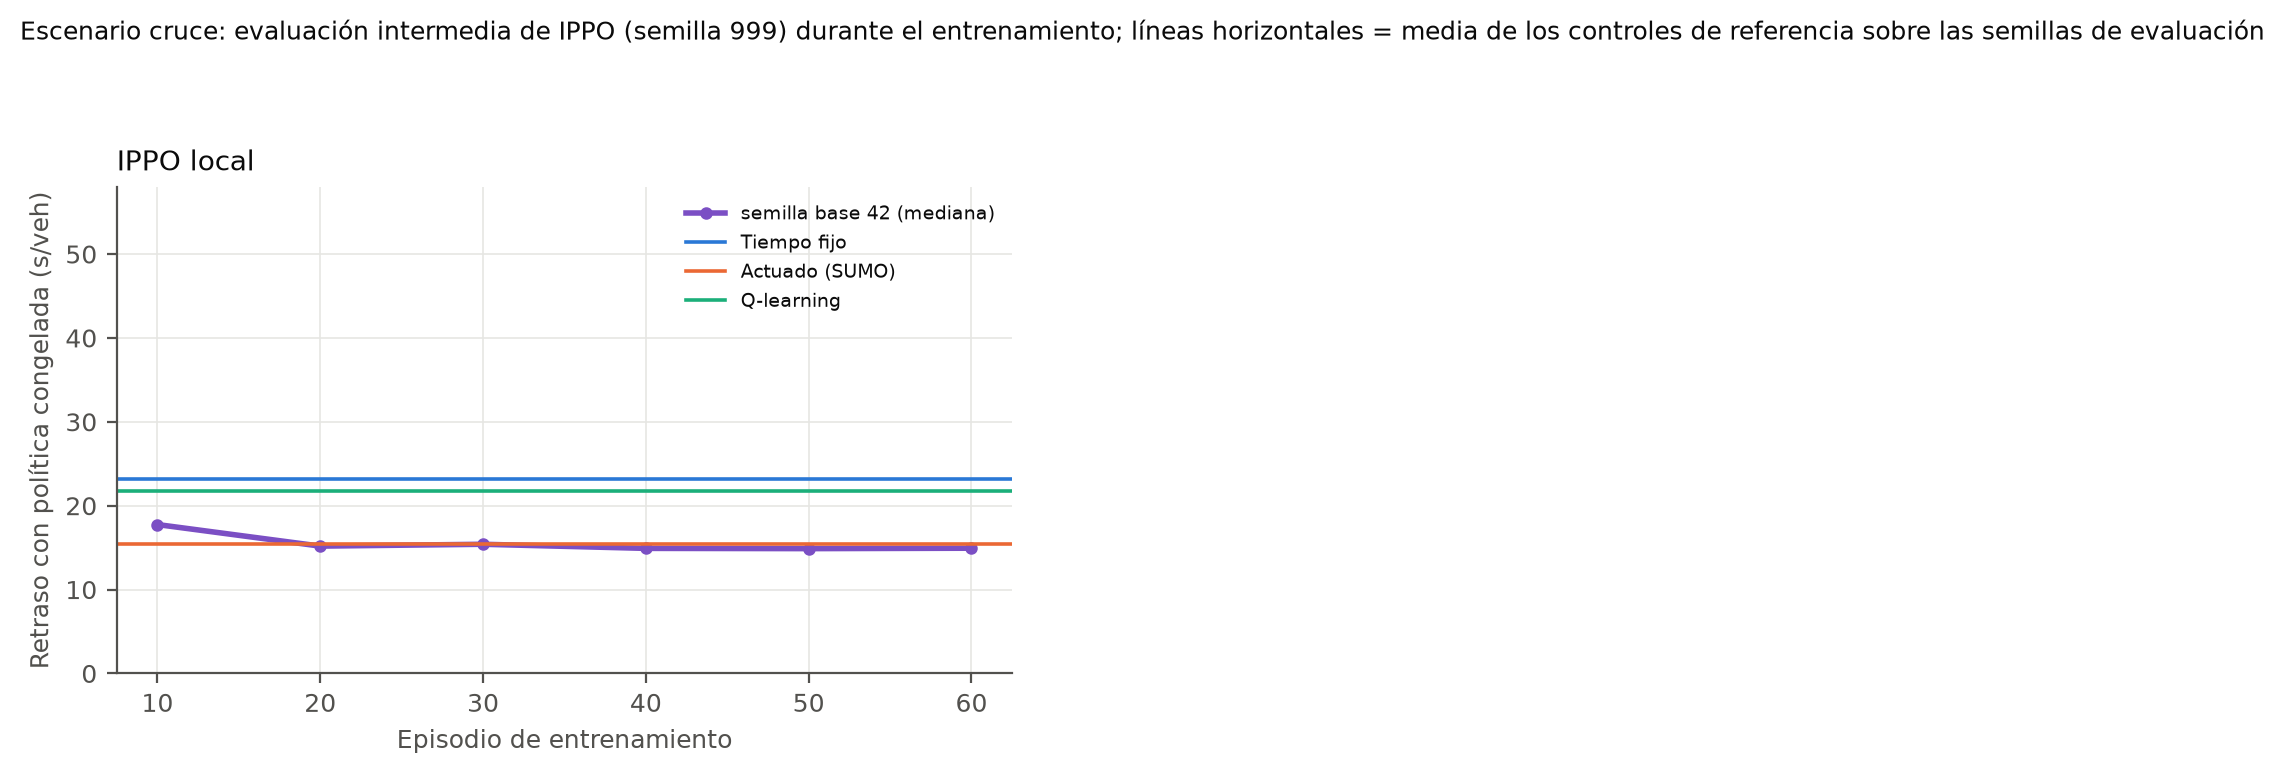
\includegraphics[width=0.62\textwidth]{fig_cruce_curva_ippo.png}
  \caption{Escenario cruce: evaluación intermedia de IPPO local con la semilla 999 durante el entrenamiento, frente a la media de los tres controles de referencia sobre las semillas de evaluación.}
  \label{fig:cruce-curva-ippo}
\end{figure}

\subsection*{Caso P4-U4: red de tres cruces con onda verde}

La red es el caso donde los agentes tabulares perdían un $15$\,\%
frente a la onda verde. Las seis políticas IPPO (dos variantes por tres
semillas base) se evaluaron junto con los tres controles de referencia
sobre las mismas diez semillas (Tablas~\ref{tab:red-u4},
\ref{tab:red-u4-deltas} y~\ref{tab:red-fragilidad},
Figuras~\ref{fig:red-curva-ippo} y~\ref{fig:red-comparacion}).

\noindent\textbf{Sin mensajería, IPPO local queda a dos puntos de la
onda verde.} La política mediana de \emph{local} da $22.17 \pm 0.23$~s,
un $+1.8$\,\% frente al fijo con intervalo $+0.7$ a $+2.9$\,\%
($p = 0.02$), cuando el agente tabular perdía un $15$\,\%. Frente a
Q-learning la mejora es de $-12$\,\% ($p = 0.002$) y frente al actuado
queda un $3.5$\,\% por encima. Pero la variante no es estable: dos
semillas base terminan en 22.1 y 22.2~s y la tercera en 24.2~s
($+11$\,\% frente al fijo), un rango de 2.1~s entre políticas, de seis
a once veces el intervalo de confianza de cualquiera de ellas. Sin
información del vecino, lo que se aprende depende de la semilla.

\noindent\textbf{Con mensajería, las tres políticas igualan a la onda
verde.} Las tres semillas base de \emph{vecinos} terminan en 21.68,
21.74 y 21.89~s frente a $21.78 \pm 0.22$~s del fijo: $-0.5$, $-0.2$ y
$+0.5$\,\%, ninguna distinguible de él ($p$ entre 0.41 y 0.85), con un
rango de 0.2~s entre ellas. La política mediana da $21.89 \pm 0.28$~s,
$+0.5$\,\% frente al fijo (intervalo $-0.3$ a $+1.3$\,\%), $-13$\,\%
frente a Q-learning y $+2.2$\,\% frente al actuado (intervalo $+0.8$ a
$+3.5$\,\%, $p = 0.02$): empata con la onda verde y queda a dos puntos
del actuado. Cada política de \emph{vecinos} es mejor que cada una de
\emph{local}, así que la ventaja de la mensajería tiene signo estable en
tres de tres. El control de no daño \emph{spill} (una semilla base),
cuyo término de \textit{spillback} nunca supera la bisagra con esta
demanda, da $21.68 \pm 0.13$~s, dentro del rango de las políticas de
\emph{vecinos}. Frente al fijo de 20/20 de la primera ronda de ajuste,
que daba 22.2~s, estas mismas políticas quedaban un $1.5$\,\% por debajo
con significancia; el reparto tuneado absorbió esa diferencia.

\noindent\textbf{Lo que la mensajería aporta es la progresión que la
onda verde ya tiene.} Las métricas de corredor lo muestran con más
claridad que el retraso global, que mezcla a los vehículos de paso con
los transversales. El fijo tuneado es ya una onda verde casi perfecta:
el $98.6$\,\% de los vehículos de paso cruza deteniéndose a lo sumo una
vez y su retraso en el sentido punta es de 24.5~s. \emph{Vecinos}
iguala esa progresión ($0.985$ y 23.6~s, un $-4$\,\% en el sentido
punta) y \emph{local} se queda algo por debajo ($0.893$ y 24.9~s); el
actuado la rompe ($0.72$ y 28.7~s) y el tabular más ($0.53$ y 36.5~s).
\emph{Vecinos} lo consigue cambiando de fase un $16$\,\% más que el
fijo, contra $+60$\,\% del actuado y $+56$\,\% del tabular, y con las
paradas por vehículo un $11$\,\% por encima del fijo, contra $+32$ y
$+76$\,\%. La
Figura~\ref{fig:red-fases} muestra el mecanismo: los tres semáforos
aprendidos mantienen la avenida en verde la mayor parte del ciclo, con
transversales cortas y regulares, y escalonan sus cambios de un cruce
al siguiente, sin que nadie les haya programado un desfase; el agente
tabular, en cambio, fragmenta el verde de la avenida. El precio está en
las transversales: el actuado, que las atiende en cuanto detecta
vehículos, sigue teniendo menos espera detenida total ($5.45$ contra
$7.53$~s) y por eso conserva la ventaja en el retraso global.

% Generado por tablas_tex.py a partir de los CSV del proyecto. No editar a mano.
\begin{table}[H]
\setstretch{1}
\centering
\scriptsize
\setlength{\tabcolsep}{3pt}
\setlength{\tabcolsep}{2pt}\begin{tabular}{p{2.8cm}rrrrrr}
\toprule
Métrica & \makecell{Fijo} & \makecell{Actuado} & \makecell{Q-learning} & \makecell{IPPO\\local} & \makecell{IPPO\\vecinos} & \makecell{IPPO\\spill} \\
\midrule
Retraso (s/veh) & 21.78 $\pm$ 0.22 & 21.42 $\pm$ 0.23 & 25.12 $\pm$ 0.31 & 22.17 $\pm$ 0.23 & 21.89 $\pm$ 0.28 & 21.68 $\pm$ 0.13 \\
Espera detenida (s/veh) & 7.41 $\pm$ 0.16 & 5.45 $\pm$ 0.19 & 7.71 $\pm$ 0.15 & 7.25 $\pm$ 0.15 & 7.53 $\pm$ 0.28 & 7.38 $\pm$ 0.10 \\
Cola promedio (veh) & 4.01 $\pm$ 0.05 & 2.93 $\pm$ 0.08 & 4.26 $\pm$ 0.11 & 3.97 $\pm$ 0.10 & 4.08 $\pm$ 0.07 & 4.03 $\pm$ 0.05 \\
Cola máxima (veh) & 14.90 $\pm$ 0.63 & 15.70 $\pm$ 1.22 & 18.20 $\pm$ 0.94 & 16.20 $\pm$ 1.25 & 13.70 $\pm$ 0.76 & 13.30 $\pm$ 0.48 \\
Paradas por vehículo & 0.61 $\pm$ 0.01 & 0.80 $\pm$ 0.01 & 1.07 $\pm$ 0.02 & 0.73 $\pm$ 0.01 & 0.68 $\pm$ 0.01 & 0.67 $\pm$ 0.01 \\
Throughput (veh) & 2095 $\pm$ 1 & 2093 $\pm$ 2 & 2091 $\pm$ 2 & 2093 $\pm$ 1 & 2093 $\pm$ 1 & 2094 $\pm$ 1 \\
CO$_2$ (g/veh) & 250.39 $\pm$ 0.47 & 256.56 $\pm$ 0.57 & 265.09 $\pm$ 0.73 & 253.53 $\pm$ 0.55 & 250.87 $\pm$ 0.50 & 250.37 $\pm$ 0.30 \\
NO$_x$ (mg/veh) & 86.46 $\pm$ 0.15 & 87.93 $\pm$ 0.18 & 90.81 $\pm$ 0.21 & 87.34 $\pm$ 0.19 & 86.58 $\pm$ 0.18 & 86.42 $\pm$ 0.11 \\
Recompensa por decisión & $-$1.43 $\pm$ 0.02 & $-$1.01 $\pm$ 0.03 & $-$1.47 $\pm$ 0.04 & $-$1.40 $\pm$ 0.04 & $-$1.46 $\pm$ 0.03 & $-$1.44 $\pm$ 0.02 \\
Cambios de fase & 489.60 $\pm$ 0.91 & 784.00 $\pm$ 4.12 & 763.30 $\pm$ 3.04 & 582.30 $\pm$ 1.47 & 569.50 $\pm$ 1.76 & 560.90 $\pm$ 1.33 \\
Viaje extremo a extremo (s) & 155.37 $\pm$ 0.46 & 160.66 $\pm$ 0.39 & 166.52 $\pm$ 0.96 & 156.90 $\pm$ 0.58 & 154.62 $\pm$ 0.26 & 154.52 $\pm$ 0.31 \\
Retraso extremo a extremo (s) & 23.45 $\pm$ 0.31 & 28.75 $\pm$ 0.36 & 34.59 $\pm$ 0.80 & 24.97 $\pm$ 0.49 & 22.70 $\pm$ 0.11 & 22.60 $\pm$ 0.19 \\
Tasa de \textit{spillback} & 0.00 $\pm$ 0.00 & 0.00 $\pm$ 0.00 & 0.00 $\pm$ 0.00 & 0.00 $\pm$ 0.00 & 0.00 $\pm$ 0.00 & 0.00 $\pm$ 0.00 \\
Cola máxima en un enlace (veh) & 1.90 $\pm$ 0.23 & 4.40 $\pm$ 0.37 & 4.80 $\pm$ 0.30 & 4.50 $\pm$ 0.38 & 2.90 $\pm$ 0.23 & 3.30 $\pm$ 0.48 \\
Retraso de paso, sentido punta (s) & 24.54 $\pm$ 0.35 & 28.67 $\pm$ 0.74 & 36.49 $\pm$ 0.94 & 24.90 $\pm$ 0.51 & 23.62 $\pm$ 0.16 & 23.38 $\pm$ 0.28 \\
Paradas de paso (/veh) & 0.48 $\pm$ 0.01 & 1.03 $\pm$ 0.02 & 1.46 $\pm$ 0.05 & 0.72 $\pm$ 0.03 & 0.56 $\pm$ 0.01 & 0.55 $\pm$ 0.01 \\
Fracción de paso con $\le 1$ parada & 0.99 $\pm$ 0.00 & 0.72 $\pm$ 0.01 & 0.53 $\pm$ 0.02 & 0.89 $\pm$ 0.01 & 0.98 $\pm$ 0.00 & 0.98 $\pm$ 0.00 \\
Segundos con \textit{spillback} & 0 $\pm$ 0 & 0 $\pm$ 0 & 0 $\pm$ 0 & 0 $\pm$ 0 & 0 $\pm$ 0 & 0 $\pm$ 0 \\
Vehículos máximos en un enlace & 9.50 $\pm$ 0.38 & 8.10 $\pm$ 0.23 & 8.70 $\pm$ 0.35 & 8.40 $\pm$ 0.37 & 8.70 $\pm$ 0.35 & 8.90 $\pm$ 0.41 \\
Vehículos no terminados & 0 $\pm$ 0 & 0 $\pm$ 0 & 0 $\pm$ 0 & 0 $\pm$ 0 & 0 $\pm$ 0 & 0 $\pm$ 0 \\
\bottomrule
\end{tabular}
\caption[Escenario red: evaluación de las variantes IPPO]{Escenario red: evaluación con política congelada sobre 10 semillas (1001 a 1010), las mismas para todos los brazos; media $\pm$ IC95\,\%. Cada variante IPPO es la política mediana de sus semillas base por la evaluación intermedia final; los cambios porcentuales están en la Tabla~\ref{tab:red-u4-deltas}.}
\label{tab:red-u4}
\end{table}
\begin{table}[H]
\setstretch{1}
\centering
\scriptsize
\setlength{\tabcolsep}{3pt}
\begin{tabular}{lrrrrrrr}
\toprule
 & Retraso & \multicolumn{3}{c}{Cambio del retraso [IC95\,\%]} & \multicolumn{3}{c}{vs fijo, secundarias} \\
\cmidrule(lr){3-5}\cmidrule(lr){6-8}
Variante & (s/veh) & vs fijo & vs actuado & vs Q-learning & Espera & Paradas & Cambios \\
\midrule
IPPO local & 22.17 & \makecell[r]{+1.8\,\%\\{}[0.7, 2.9]\\$p$ = 0.0195} & \makecell[r]{+3.5\,\%\\{}[2.7, 4.4]\\$p$ = 0.00195} & \makecell[r]{$-$11.7\,\%\\{}[$-$12.7, $-$10.6]\\$p$ = 0.00195} & $-$2.2\,\% & +19.8\,\% & +18.9\,\% \\
IPPO vecinos & 21.89 & \makecell[r]{+0.5\,\%\\{}[$-$0.3, 1.3]\\$p$ = 0.414} & \makecell[r]{+2.2\,\%\\{}[0.8, 3.5]\\$p$ = 0.0195} & \makecell[r]{$-$12.9\,\%\\{}[$-$14.1, $-$11.6]\\$p$ = 0.00195} & +1.6\,\% & +11.1\,\% & +16.3\,\% \\
IPPO spill & 21.68 & \makecell[r]{$-$0.5\,\%\\{}[$-$1.7, 0.6]\\$p$ = 0.846} & \makecell[r]{+1.2\,\%\\{}[0.2, 2.1]\\$p$ = 0.0371} & \makecell[r]{$-$13.7\,\%\\{}[$-$14.7, $-$12.7]\\$p$ = 0.00195} & $-$0.5\,\% & +9.0\,\% & +14.6\,\% \\
\bottomrule
\end{tabular}
\caption[Escenario red: cambio del retraso de las variantes IPPO]{Escenario red: cambio porcentual del retraso de cada variante IPPO (política mediana) frente al fijo, al actuado y a Q-learning, con intervalo bootstrap pareado por semilla y $p$ de Wilcoxon pareado; a la derecha, cambio frente al fijo de tres secundarias.}
\label{tab:red-u4-deltas}
\end{table}

% Generado por tablas_tex.py a partir de los CSV del proyecto. No editar a mano.
\begin{table}[H]
\setstretch{1}
\centering
\scriptsize
\setlength{\tabcolsep}{3pt}
\begin{tabular}{llrrrr}
\toprule
Variante & Semilla base & \makecell{Eval. intermedia\\final (s/veh)} & \makecell{Retraso, semillas\\de evaluación (s/veh)} & $\Delta$ vs fijo [IC95\,\%] & $p$ \\
\midrule
IPPO local & 42 & 23.54 & 24.20 $\pm$ 0.37 & +11.1\,\% [9.2, 13.1] & 0.00195 \\
IPPO local & 2042 (mediana) & 22.26 & 22.17 $\pm$ 0.23 & +1.8\,\% [0.7, 2.9] & 0.0195 \\
IPPO local & 4042 & 21.76 & 22.09 $\pm$ 0.20 & +1.4\,\% [0.3, 2.2] & 0.0449 \\
 & rango entre bases & & 2.11 & & \\
IPPO vecinos & 42 & 21.94 & 21.68 $\pm$ 0.13 & $-$0.5\,\% [$-$1.7, 0.6] & 0.846 \\
IPPO vecinos & 2042 & 21.52 & 21.74 $\pm$ 0.20 & $-$0.2\,\% [$-$1.1, 0.8] & 0.82 \\
IPPO vecinos & 4042 (mediana) & 21.66 & 21.89 $\pm$ 0.28 & +0.5\,\% [$-$0.3, 1.3] & 0.414 \\
 & rango entre bases & & 0.20 & & \\
IPPO spill & 42 (mediana) & 21.94 & 21.68 $\pm$ 0.13 & $-$0.5\,\% [$-$1.7, 0.6] & 0.846 \\
\bottomrule
\end{tabular}
\caption[Escenario red: fragilidad del entrenamiento IPPO]{Escenario red: las tres políticas de cada variante IPPO. La evaluación intermedia final usa la semilla 999; la media, las semillas de evaluación. El rango entre bases se compara con el IC95\,\% de una sola política.}
\label{tab:red-fragilidad}
\end{table}


\begin{figure}[H]
  \centering
  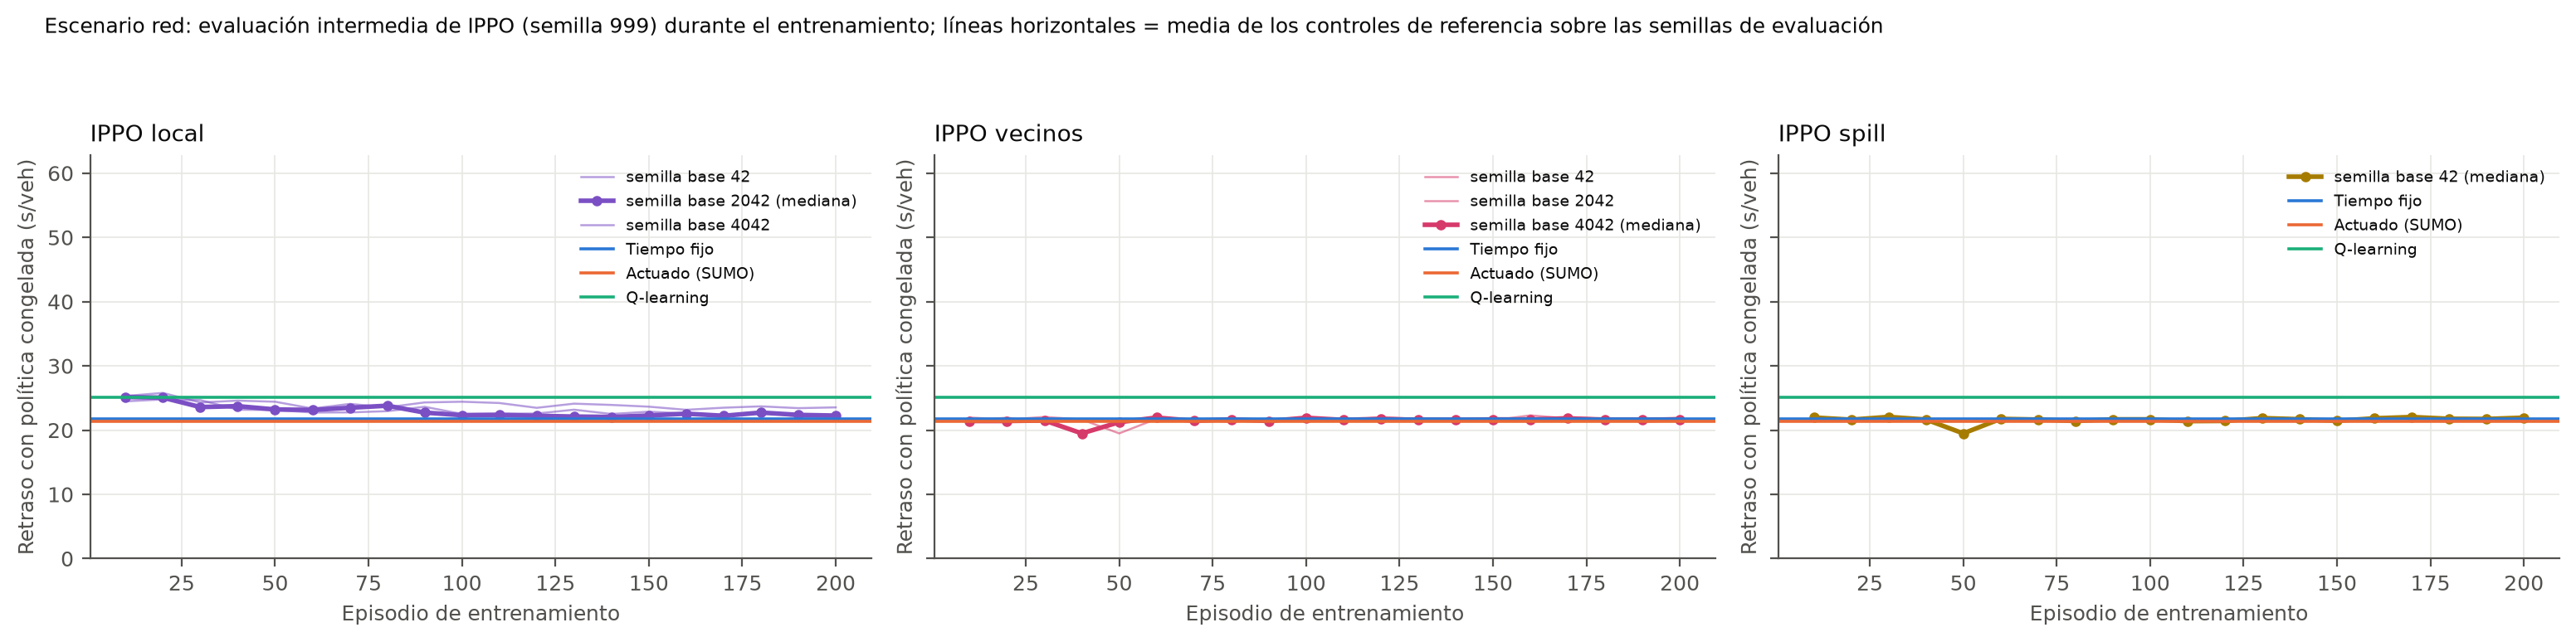
\includegraphics[width=0.95\textwidth]{fig_red_curva_ippo.png}
  \caption{Escenario red: evaluación intermedia de las tres políticas de cada variante IPPO durante el entrenamiento (semilla 999); en trazo grueso, la política mediana.}
  \label{fig:red-curva-ippo}
\end{figure}

\begin{figure}[H]
  \centering
  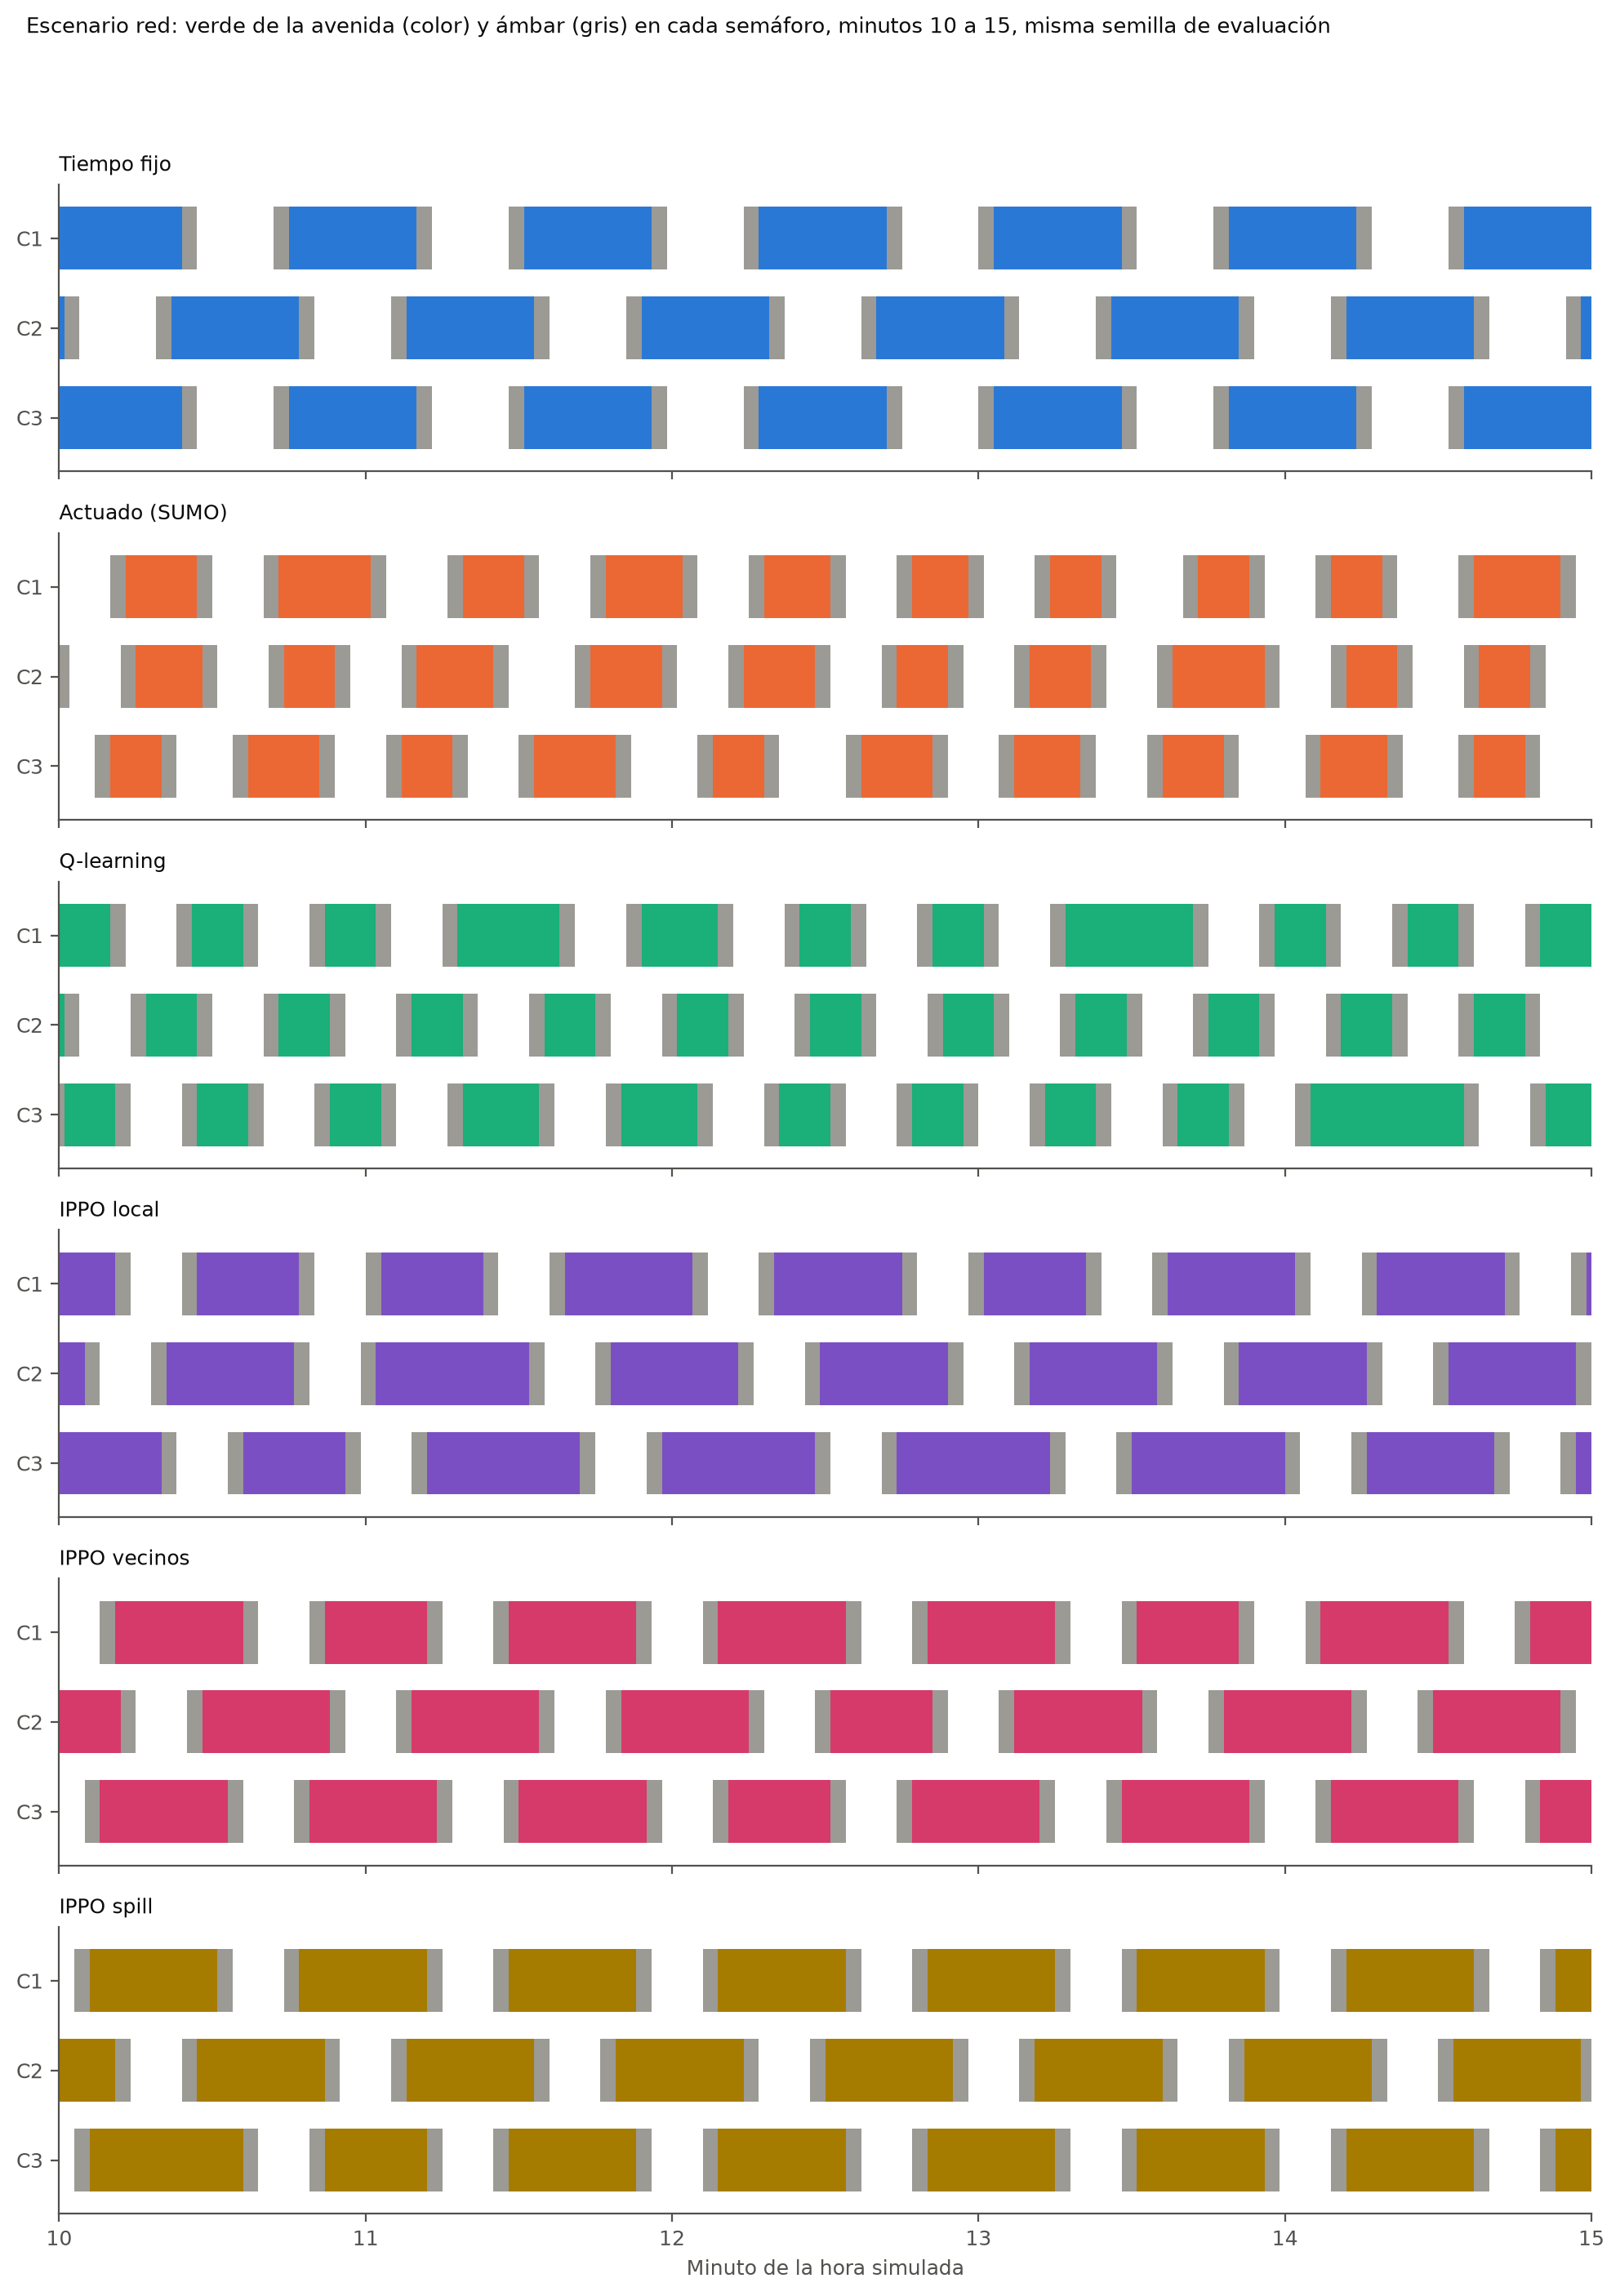
\includegraphics[width=0.95\textwidth]{fig_red_fases.png}
  \caption{Escenario red: verde de la avenida en cada semáforo durante cinco minutos del periodo punta, con la misma semilla, bajo el fijo con onda verde, el actuado, Q-learning e IPPO.}
  \label{fig:red-fases}
\end{figure}

\noindent\textbf{Canal imperfecto.} La política mediana de \emph{vecinos},
entrenada con mensajes instantáneos, se evaluó sin reentrenar con
latencia y pérdida de mensajes (Tabla~\ref{tab:red-s1}). Con latencia
de 5~s y pérdida del 30\,\% pierde 0.8~s de retraso frente al canal
perfecto ($22.70$ contra $21.89$~s), dentro del límite de 2~s del
criterio de robustez pero ya un $4$\,\% por detrás del fijo tuneado;
con latencia de 10~s pierde 2.2~s y queda un $10$\,\% por detrás del
fijo. Pero el retraso global esconde lo que cambia: con
cualquier canal imperfecto la progresión se deshace (la fracción de
vehículos de paso con a lo sumo una parada baja de 0.985 a entre 0.54 y
0.80, y el retraso en el sentido punta sube de 23.6 a entre 27.7 y
32.7~s) y los semáforos cambian de fase entre un $29$ y un $39$\,\%
más, como el actuado. Con latencia de 5~s sin pérdida el retraso global
incluso baja a 21.19~s, pero por el camino contrario al aprendido: más
cambios y menos progresión, más parecido al actuado. La lectura es que
el agente usa el mensaje del vecino tal cual, sin descontarlo por su
edad, porque durante el entrenamiento nunca vio un mensaje viejo: la
edad del mensaje está en la observación, pero fuera del rango
entrenado no informa. Entrenar con latencia variable es la corrección
natural y queda en las recomendaciones.

% Generado por tablas_tex.py a partir de los CSV del proyecto. No editar a mano.
\begin{table}[H]
\setstretch{1}
\centering
\scriptsize
\setlength{\tabcolsep}{3pt}
\begin{tabular}{lrrrrr}
\toprule
Canal & Retraso (s/veh) & \makecell{Diferencia vs\\perfecto (s)} & \makecell{Paso con\\$\le 1$ parada} & \makecell{Retraso de paso\\punta (s)} & Cambios \\
\midrule
canal perfecto & 21.89 $\pm$ 0.28 & -- & 0.985 & 23.6 & 569.5 \\
latencia 5~s & 21.19 $\pm$ 0.26 & $-$0.70 $\pm$ 0.26 & 0.795 & 27.7 & 791.7 \\
latencia 5~s, pérdida 30\,\% & 22.70 $\pm$ 0.23 & +0.81 $\pm$ 0.31 & 0.705 & 29.7 & 753.6 \\
latencia 10~s & 24.04 $\pm$ 0.12 & +2.16 $\pm$ 0.27 & 0.542 & 32.7 & 734.4 \\
\bottomrule
\end{tabular}
\caption[Escenario red: IPPO vecinos con canal imperfecto]{Escenario red: la política mediana de IPPO vecinos evaluada con latencia y pérdida de mensajes, sin reentrenar, sobre las mismas semillas. La diferencia frente al canal perfecto es la media pareada por semilla $\pm$ IC95\,\%.}
\label{tab:red-s1}
\end{table}


\subsection*{Caso P3-U4: corredor de dos cruces}

En el corredor el agente tabular pierde un $60$\,\% frente al fijo de
reparto tuneado, que da $21.2 \pm 0.4$~s, y el actuado empata con él.
Las siete políticas IPPO (dos variantes por tres semillas base, más
\emph{spill} con una base como control de no daño) se evaluaron con
los tres controles de referencia sobre las mismas diez semillas
(Tablas~\ref{tab:corredor-u4}, \ref{tab:corredor-u4-deltas}
y~\ref{tab:corredor-fragilidad}, Figuras~\ref{fig:corredor-curva-ippo},
\ref{fig:corredor-comparacion} y~\ref{fig:corredor-fases}).

\noindent\textbf{Sin mensajería, IPPO local iguala al fijo tuneado y al
actuado.} La política mediana de \emph{local} da $21.27 \pm 0.33$~s,
un $+0.6$\,\% frente al fijo con intervalo $-1.1$ a $+2.2$\,\%
($p = 0.58$); las tres semillas base quedan en $+0.1$, $+0.6$ y
$-2.4$\,\%. Frente al actuado la diferencia es de $+1.7$\,\% con
intervalo $+0.2$ a $+3.3$\,\% y $p = 0.125$: queda apenas por encima,
la prueba pareada no distingue ambos controles pero el intervalo no
incluye el cero. Frente a Q-learning la mejora es de $-37$\,\%.

\noindent\textbf{Con mensajería, las tres políticas superan al fijo
tuneado y al actuado.} La política mediana de \emph{vecinos} da
$19.84 \pm 0.37$~s, $-6.2$\,\% frente al fijo (intervalo $-8.0$ a
$-4.6$\,\%, $p = 0.002$) y $-5.1$\,\% frente al actuado (intervalo
$-6.4$ a $-3.9$\,\%, $p = 0.002$). Las tres semillas base quedan por
debajo de los dos, con retrasos de 19.84, 19.90 y 20.37~s, y cada una
es mejor que cada política de \emph{local}. Es el primer control
aprendido que supera al actuado en un escenario de varios cruces. El
control de no daño \emph{spill}, con el término de \textit{spillback}
que aquí nunca se activa por encima de la bisagra, queda en
$20.21 \pm 0.29$~s, dentro del rango de las políticas de
\emph{vecinos}. Ninguna variante alcanza la meta de $-25$\,\%: la
cola promedio baja un $5.6$\,\% y el CO$_2$ un $1.6$\,\% frente al
fijo, lejos también de sus metas. Frente al fijo simétrico de 25/25 que
se usó en la primera ronda de ajuste, estas mismas políticas mostraban
$-38$\,\% de retraso, $-50$\,\% de colas y $-10$\,\% de CO$_2$: la
diferencia entre las dos lecturas mide cuánto pesaba el reparto de
verde de la referencia, no lo que hace el agente. Lo que sí es
independiente de la referencia fija es la comparación con el actuado,
que no cambió.

\noindent\textbf{Cómo lo consigue.} El fijo tuneado ya forma una onda
verde eficaz: el $91$\,\% de los vehículos de paso cruza deteniéndose a
lo sumo una vez y el retraso en el sentido punta es de 24~s, contra
$60$\,\% y 46~s del programa simétrico. Sobre esa base, \emph{vecinos}
sube la fracción a $0.95$ (actuado $0.73$, Q-learning $0.32$), baja el
retraso en el sentido punta a 20~s ($-17$\,\%; el actuado lo sube a
26~s) y reduce la cola máxima del enlace entre cruces de 8 a 5.5
vehículos ($-30$\,\%; el actuado deja 7). Las paradas por vehículo
bajan un $16$\,\% frente al fijo y un $19$\,\% frente al actuado, y lo
hace cambiando de fase un $10$\,\% menos que el fijo y un $19$\,\%
menos que el actuado; la espera detenida queda un $10$\,\% por encima
de la del actuado, que sigue siendo el control que menos detiene. Como
en la red, el agente con mensajes abre la avenida en pelotón de un
cruce al siguiente (Figura~\ref{fig:corredor-fases}). La variante
\emph{local} llega a lo mismo que el fijo con detectores propios: en un
corredor de dos cruces separados 300~m el pelotón que sale del primero
es visible para el segundo en su propia aproximación; la mensajería
añade los seis puntos que separan a \emph{vecinos} de \emph{local}.

% Generado por tablas_tex.py a partir de los CSV del proyecto. No editar a mano.
\begin{table}[H]
\setstretch{1}
\centering
\scriptsize
\setlength{\tabcolsep}{3pt}
\setlength{\tabcolsep}{2pt}\begin{tabular}{p{2.8cm}rrrrrr}
\toprule
Métrica & \makecell{Fijo} & \makecell{Actuado} & \makecell{Q-learning} & \makecell{IPPO\\local} & \makecell{IPPO\\vecinos} & \makecell{IPPO\\spill} \\
\midrule
Retraso (s/veh) & 21.15 $\pm$ 0.41 & 20.91 $\pm$ 0.25 & 33.86 $\pm$ 1.66 & 21.27 $\pm$ 0.33 & 19.84 $\pm$ 0.36 & 20.21 $\pm$ 0.28 \\
Espera detenida (s/veh) & 6.97 $\pm$ 0.18 & 5.90 $\pm$ 0.14 & 12.27 $\pm$ 0.50 & 7.37 $\pm$ 0.20 & 6.52 $\pm$ 0.23 & 6.77 $\pm$ 0.16 \\
Cola promedio (veh) & 3.81 $\pm$ 0.08 & 3.32 $\pm$ 0.07 & 6.38 $\pm$ 0.23 & 4.01 $\pm$ 0.10 & 3.60 $\pm$ 0.11 & 3.72 $\pm$ 0.08 \\
Cola máxima (veh) & 16.10 $\pm$ 1.52 & 16.70 $\pm$ 1.01 & 22.40 $\pm$ 1.66 & 15.20 $\pm$ 0.56 & 14.10 $\pm$ 0.53 & 14.80 $\pm$ 1.11 \\
Paradas por vehículo & 0.80 $\pm$ 0.02 & 0.83 $\pm$ 0.02 & 1.54 $\pm$ 0.08 & 0.77 $\pm$ 0.02 & 0.67 $\pm$ 0.01 & 0.68 $\pm$ 0.01 \\
Throughput (veh) & 1770 $\pm$ 1 & 1766 $\pm$ 1 & 1758 $\pm$ 4 & 1767 $\pm$ 2 & 1768 $\pm$ 2 & 1768 $\pm$ 2 \\
CO$_2$ (g/veh) & 219.76 $\pm$ 0.82 & 221.59 $\pm$ 0.59 & 244.32 $\pm$ 2.70 & 219.27 $\pm$ 0.75 & 216.27 $\pm$ 0.78 & 217.22 $\pm$ 0.60 \\
NO$_x$ (mg/veh) & 75.59 $\pm$ 0.27 & 75.94 $\pm$ 0.18 & 83.81 $\pm$ 0.92 & 75.52 $\pm$ 0.27 & 74.49 $\pm$ 0.27 & 74.79 $\pm$ 0.21 \\
Recompensa por decisión & $-$1.87 $\pm$ 0.04 & $-$1.58 $\pm$ 0.04 & $-$3.22 $\pm$ 0.12 & $-$1.99 $\pm$ 0.06 & $-$1.76 $\pm$ 0.06 & $-$1.83 $\pm$ 0.05 \\
Cambios de fase & 410.40 $\pm$ 0.37 & 459.30 $\pm$ 4.17 & 462.70 $\pm$ 3.04 & 369.10 $\pm$ 2.12 & 371.60 $\pm$ 1.02 & 366.90 $\pm$ 1.45 \\
Viaje extremo a extremo (s) & 105.82 $\pm$ 0.82 & 108.22 $\pm$ 0.50 & 131.81 $\pm$ 2.89 & 104.55 $\pm$ 0.40 & 102.35 $\pm$ 0.42 & 102.23 $\pm$ 0.53 \\
Retraso extremo a extremo (s) & 22.88 $\pm$ 0.77 & 25.27 $\pm$ 0.44 & 48.87 $\pm$ 2.89 & 21.61 $\pm$ 0.37 & 19.42 $\pm$ 0.38 & 19.29 $\pm$ 0.48 \\
Tasa de \textit{spillback} & 0.00 $\pm$ 0.00 & 0.00 $\pm$ 0.00 & 0.00 $\pm$ 0.00 & 0.00 $\pm$ 0.00 & 0.00 $\pm$ 0.00 & 0.00 $\pm$ 0.00 \\
Cola máxima en un enlace (veh) & 7.90 $\pm$ 0.92 & 7.20 $\pm$ 0.45 & 10.90 $\pm$ 1.09 & 6.50 $\pm$ 0.61 & 5.50 $\pm$ 1.23 & 5.40 $\pm$ 0.84 \\
Retraso de paso, sentido punta (s) & 24.39 $\pm$ 1.16 & 26.49 $\pm$ 0.56 & 58.01 $\pm$ 4.02 & 22.89 $\pm$ 0.53 & 20.34 $\pm$ 0.45 & 20.13 $\pm$ 0.53 \\
Paradas de paso (/veh) & 0.81 $\pm$ 0.04 & 1.00 $\pm$ 0.03 & 2.24 $\pm$ 0.14 & 0.77 $\pm$ 0.03 & 0.60 $\pm$ 0.02 & 0.59 $\pm$ 0.02 \\
Fracción de paso con $\le 1$ parada & 0.91 $\pm$ 0.01 & 0.73 $\pm$ 0.02 & 0.32 $\pm$ 0.01 & 0.90 $\pm$ 0.01 & 0.95 $\pm$ 0.01 & 0.95 $\pm$ 0.01 \\
Segundos con \textit{spillback} & 0 $\pm$ 0 & 0 $\pm$ 0 & 0 $\pm$ 0 & 0 $\pm$ 0 & 0 $\pm$ 0 & 0 $\pm$ 0 \\
Vehículos máximos en un enlace & 14.60 $\pm$ 1.48 & 12.30 $\pm$ 0.59 & 24.20 $\pm$ 2.69 & 11.80 $\pm$ 0.56 & 11.80 $\pm$ 0.66 & 11.20 $\pm$ 0.74 \\
Vehículos no terminados & 0 $\pm$ 0 & 0 $\pm$ 0 & 0 $\pm$ 0 & 0 $\pm$ 0 & 0 $\pm$ 0 & 0 $\pm$ 0 \\
\bottomrule
\end{tabular}
\caption[Escenario corredor: evaluación de las variantes IPPO]{Escenario corredor: evaluación con política congelada sobre 10 semillas (1001 a 1010), las mismas para todos los brazos; media $\pm$ IC95\,\%. Cada variante IPPO es la política mediana de sus semillas base por la evaluación intermedia final; los cambios porcentuales están en la Tabla~\ref{tab:corredor-u4-deltas}.}
\label{tab:corredor-u4}
\end{table}
\begin{table}[H]
\setstretch{1}
\centering
\scriptsize
\setlength{\tabcolsep}{3pt}
\begin{tabular}{lrrrrrrr}
\toprule
 & Retraso & \multicolumn{3}{c}{Cambio del retraso [IC95\,\%]} & \multicolumn{3}{c}{vs fijo, secundarias} \\
\cmidrule(lr){3-5}\cmidrule(lr){6-8}
Variante & (s/veh) & vs fijo & vs actuado & vs Q-learning & Espera & Paradas & Cambios \\
\midrule
IPPO local & 21.27 & \makecell[r]{+0.6\,\%\\{}[$-$1.1, 2.2]\\$p$ = 0.576} & \makecell[r]{+1.7\,\%\\{}[0.2, 3.3]\\$p$ = 0.125} & \makecell[r]{$-$37.2\,\%\\{}[$-$40.1, $-$34.1]\\$p$ = 0.00195} & +5.7\,\% & $-$2.8\,\% & $-$10.1\,\% \\
IPPO vecinos & 19.84 & \makecell[r]{$-$6.2\,\%\\{}[$-$8.0, $-$4.6]\\$p$ = 0.00195} & \makecell[r]{$-$5.1\,\%\\{}[$-$6.4, $-$3.9]\\$p$ = 0.00195} & \makecell[r]{$-$41.4\,\%\\{}[$-$43.8, $-$39.0]\\$p$ = 0.00195} & $-$6.5\,\% & $-$15.9\,\% & $-$9.5\,\% \\
IPPO spill & 20.21 & \makecell[r]{$-$4.4\,\%\\{}[$-$5.7, $-$3.1]\\$p$ = 0.00195} & \makecell[r]{$-$3.3\,\%\\{}[$-$4.8, $-$2.0]\\$p$ = 0.00391} & \makecell[r]{$-$40.3\,\%\\{}[$-$42.9, $-$37.6]\\$p$ = 0.00195} & $-$3.0\,\% & $-$15.1\,\% & $-$10.6\,\% \\
\bottomrule
\end{tabular}
\caption[Escenario corredor: cambio del retraso de las variantes IPPO]{Escenario corredor: cambio porcentual del retraso de cada variante IPPO (política mediana) frente al fijo, al actuado y a Q-learning, con intervalo bootstrap pareado por semilla y $p$ de Wilcoxon pareado; a la derecha, cambio frente al fijo de tres secundarias.}
\label{tab:corredor-u4-deltas}
\end{table}

% Generado por tablas_tex.py a partir de los CSV del proyecto. No editar a mano.
\begin{table}[H]
\setstretch{1}
\centering
\scriptsize
\setlength{\tabcolsep}{3pt}
\begin{tabular}{llrrrr}
\toprule
Variante & Semilla base & \makecell{Eval. intermedia\\final (s/veh)} & \makecell{Retraso, semillas\\de evaluación (s/veh)} & $\Delta$ vs fijo [IC95\,\%] & $p$ \\
\midrule
IPPO local & 42 & 20.50 & 20.64 $\pm$ 0.26 & $-$2.4\,\% [$-$3.5, $-$1.2] & 0.00977 \\
IPPO local & 2042 (mediana) & 20.83 & 21.27 $\pm$ 0.33 & +0.6\,\% [$-$1.1, 2.2] & 0.576 \\
IPPO local & 4042 & 21.71 & 21.18 $\pm$ 0.29 & +0.1\,\% [$-$1.5, 1.7] & 0.922 \\
 & rango entre bases & & 0.64 & & \\
IPPO vecinos & 42 (mediana) & 20.23 & 19.84 $\pm$ 0.36 & $-$6.2\,\% [$-$8.0, $-$4.6] & 0.00195 \\
IPPO vecinos & 2042 & 19.79 & 19.90 $\pm$ 0.38 & $-$5.9\,\% [$-$7.2, $-$4.7] & 0.00195 \\
IPPO vecinos & 4042 & 20.70 & 20.37 $\pm$ 0.40 & $-$3.7\,\% [$-$5.5, $-$1.8] & 0.00977 \\
 & rango entre bases & & 0.54 & & \\
IPPO spill & 42 (mediana) & 20.83 & 20.21 $\pm$ 0.28 & $-$4.4\,\% [$-$5.7, $-$3.1] & 0.00195 \\
\bottomrule
\end{tabular}
\caption[Escenario corredor: fragilidad del entrenamiento IPPO]{Escenario corredor: las tres políticas de cada variante IPPO. La evaluación intermedia final usa la semilla 999; la media, las semillas de evaluación. El rango entre bases se compara con el IC95\,\% de una sola política.}
\label{tab:corredor-fragilidad}
\end{table}


\begin{figure}[H]
  \centering
  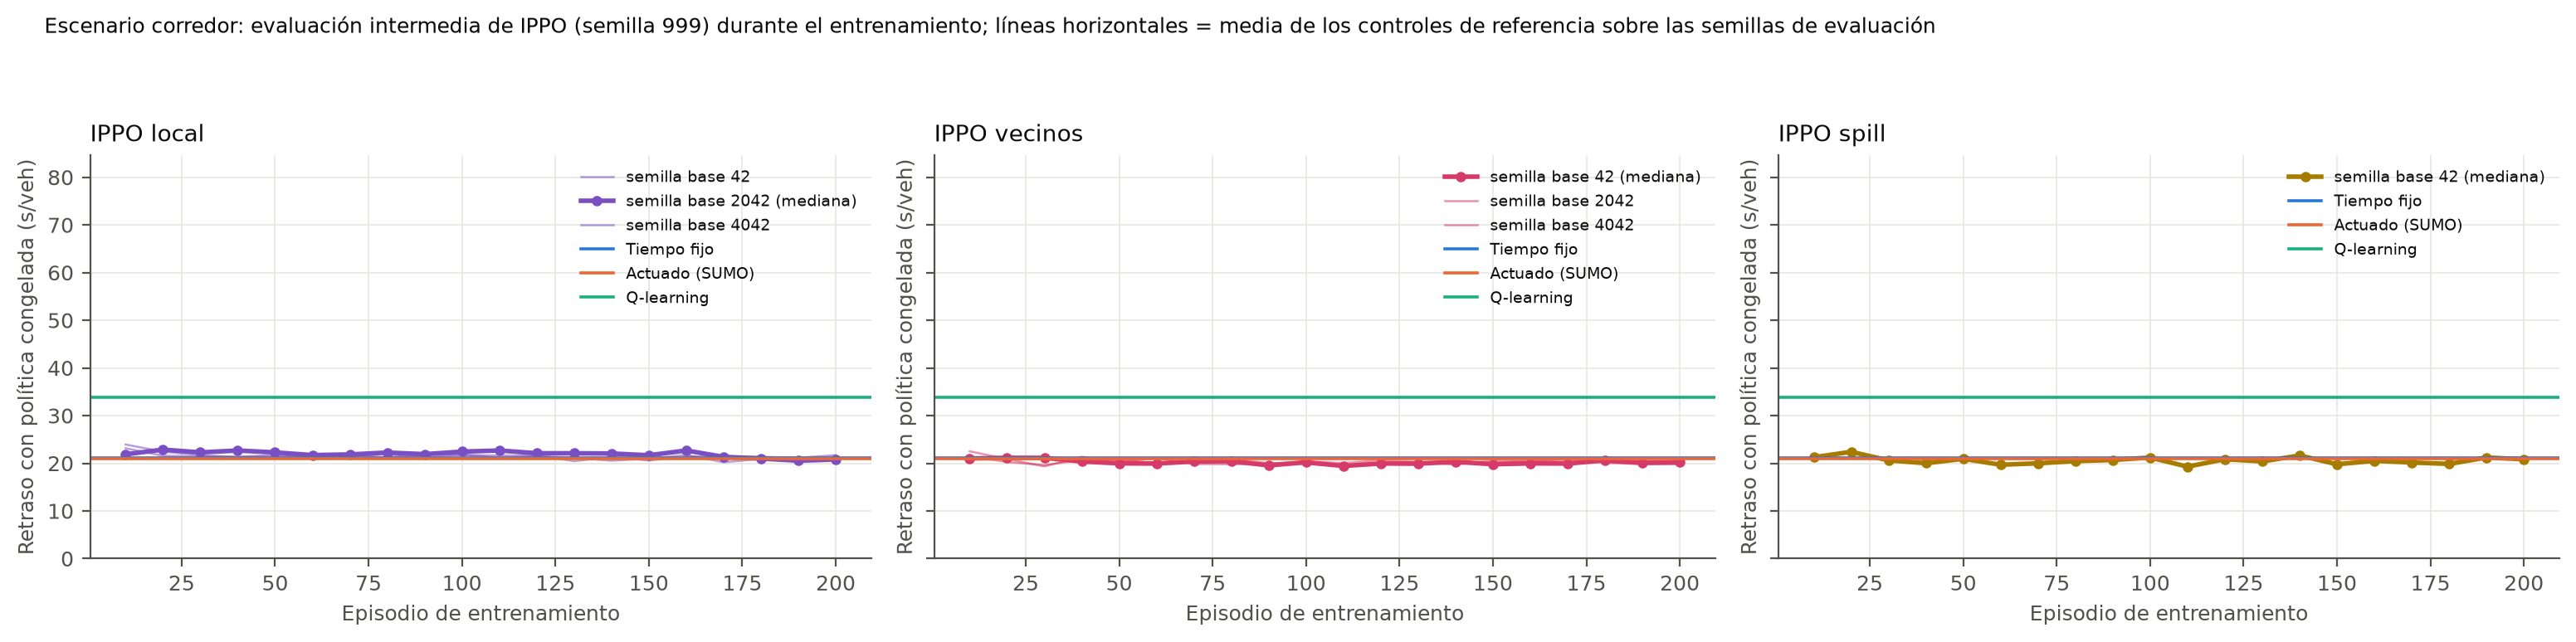
\includegraphics[width=0.95\textwidth]{fig_corredor_curva_ippo.png}
  \caption{Escenario corredor: evaluación intermedia de las políticas IPPO durante el entrenamiento (semilla 999); en trazo grueso, la política mediana de cada variante.}
  \label{fig:corredor-curva-ippo}
\end{figure}

\begin{figure}[H]
  \centering
  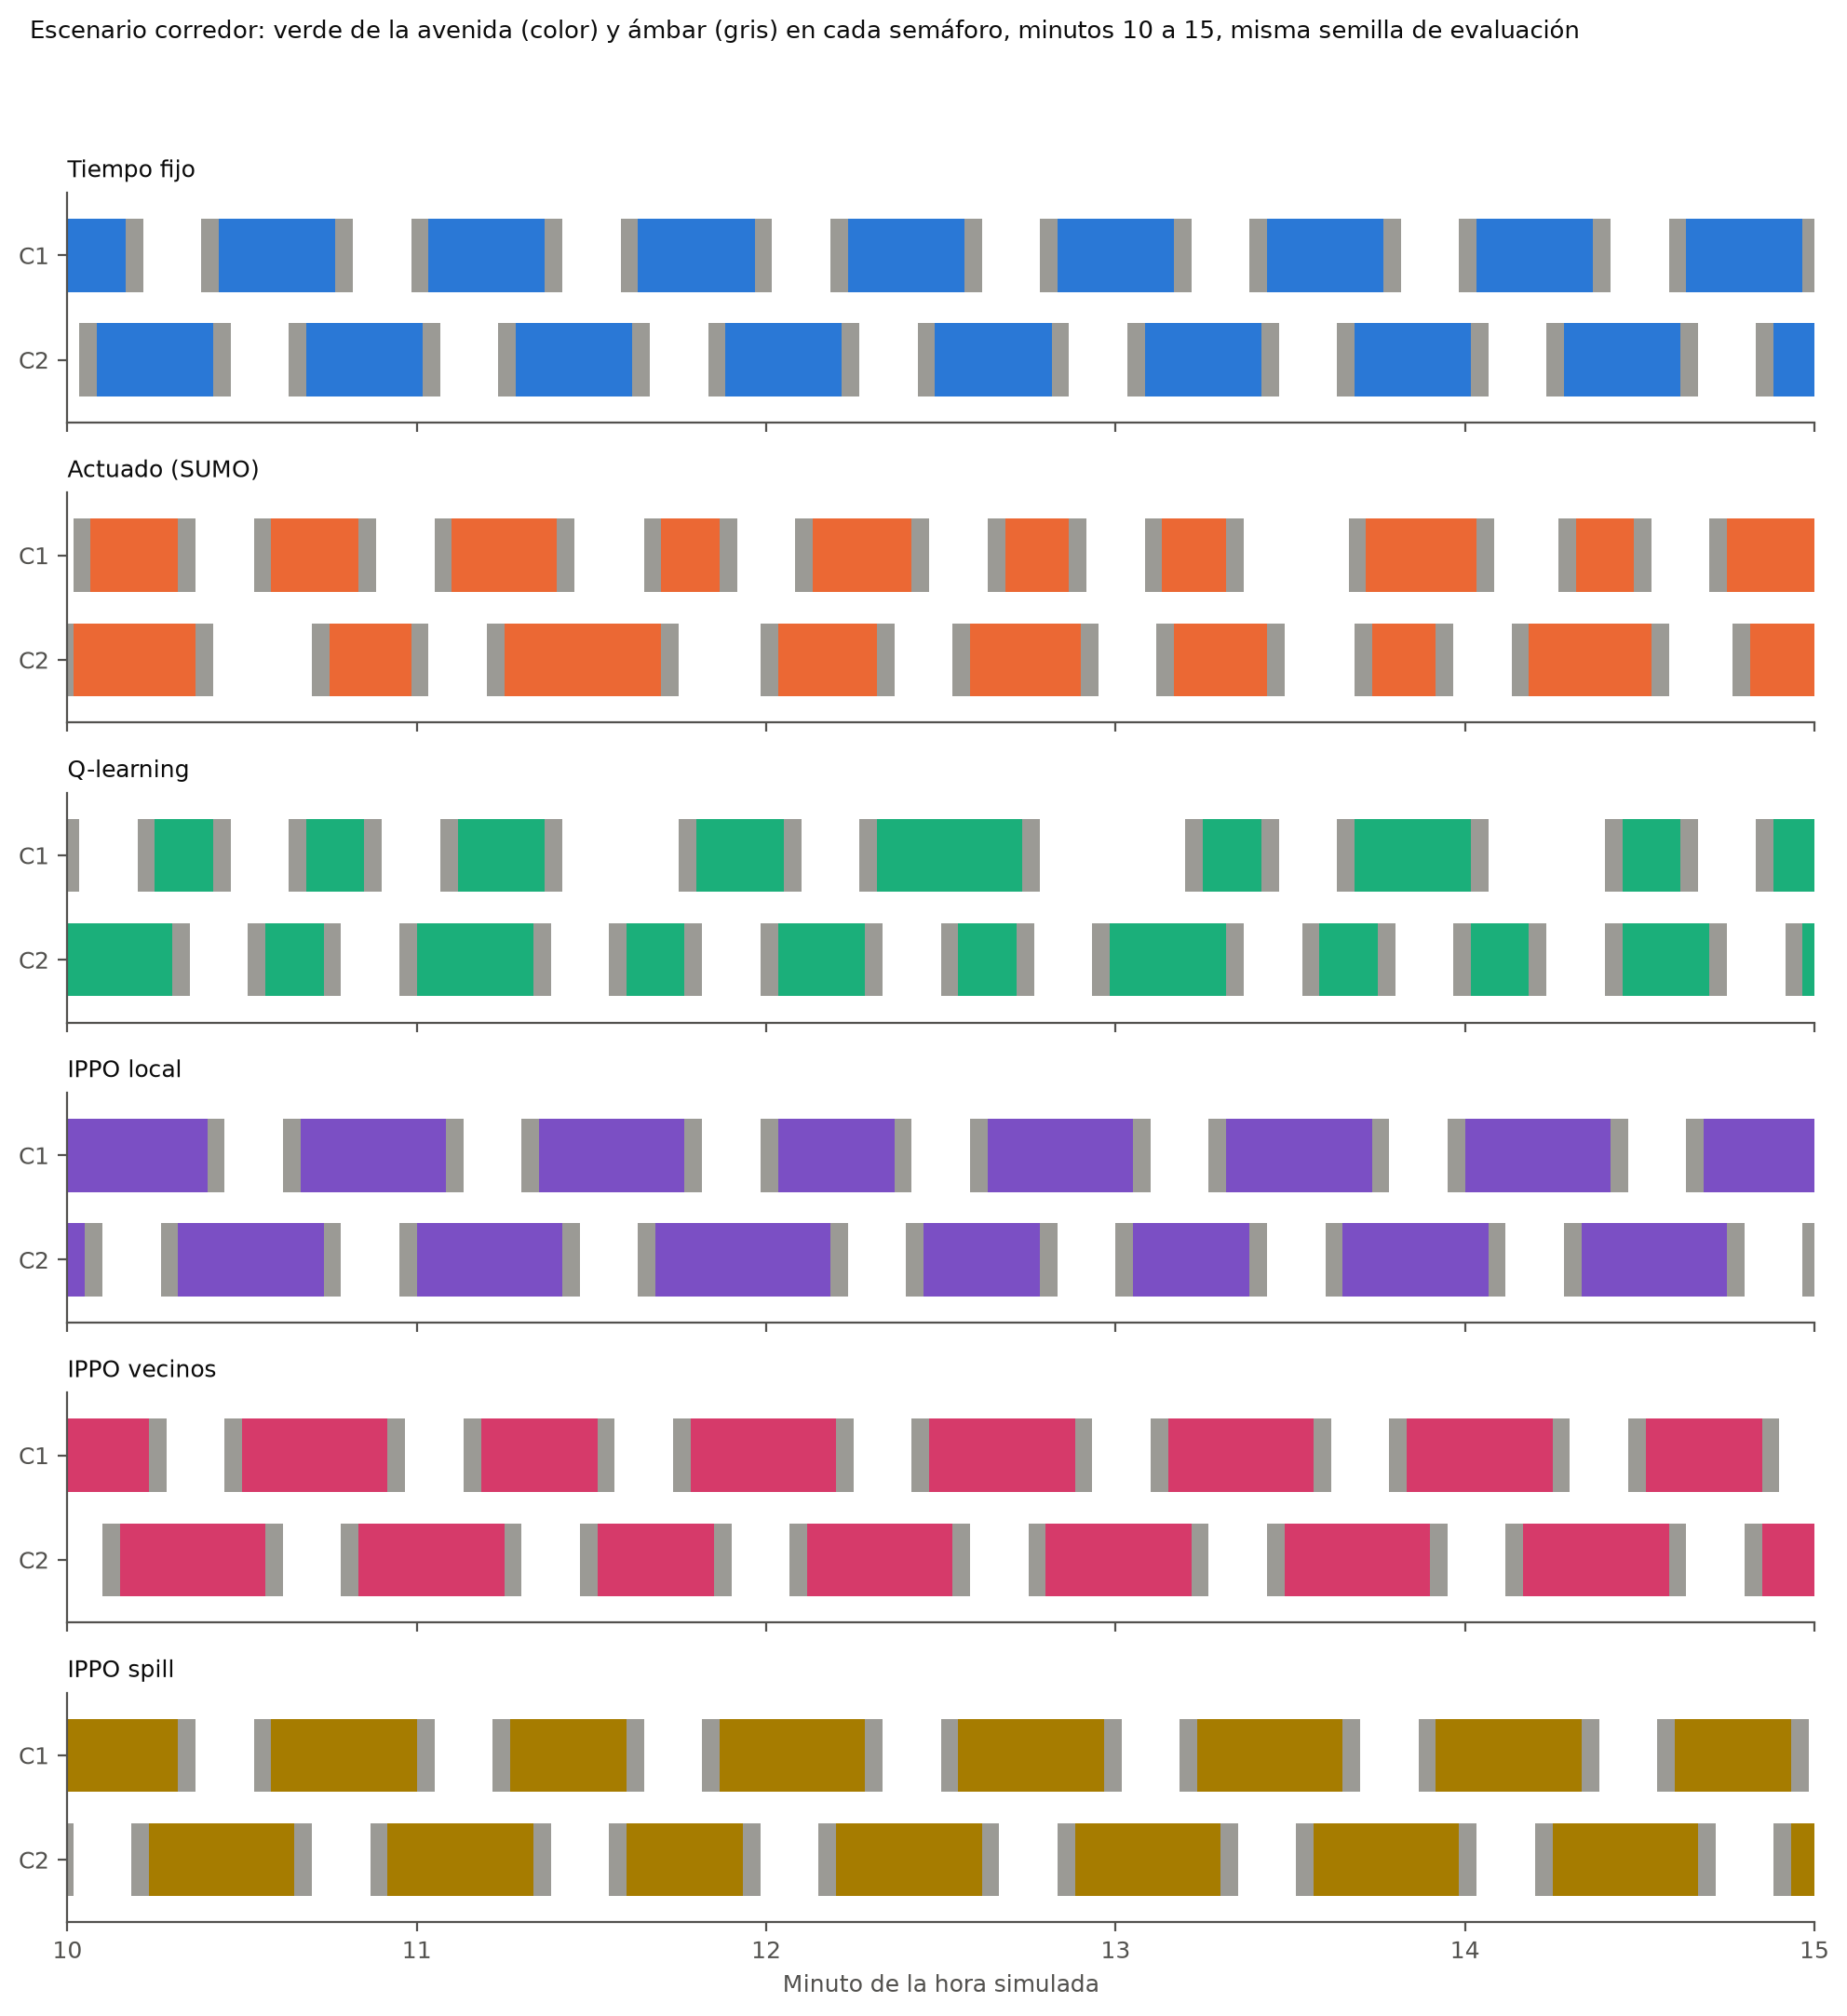
\includegraphics[width=0.95\textwidth]{fig_corredor_fases.png}
  \caption{Escenario corredor: verde de la avenida en cada semáforo durante cinco minutos del periodo punta, misma semilla, bajo cada control.}
  \label{fig:corredor-fases}
\end{figure}

\noindent\textbf{Canal imperfecto.} En el corredor la política mediana
de \emph{vecinos} pierde 1.4~s con latencia de 5~s, 2.2~s con
latencia de 5~s y pérdida del 30\,\%, y 2.5~s con latencia de 10~s
(Tabla~\ref{tab:corredor-s1}); el límite de 2~s del criterio de
robustez se supera por poco en la configuración de referencia. En los
tres casos el retraso sigue muy por debajo del fijo, pero deja de
igualar al actuado: queda un $1.7$\,\% por encima con latencia de 5~s
(intervalo $+0.6$ a $+2.8$\,\%), un $5.4$\,\% con latencia y pérdida y
un $7$\,\% con latencia de 10~s; y, como en la red, la progresión se
degrada: la fracción de vehículos de paso con a lo sumo una parada baja
de 0.95 a entre 0.65 y 0.85 y el retraso en el sentido punta sube de
20 a entre 24 y 28~s. La política depende del mensaje del vecino y no
aprendió a desconfiar de un mensaje viejo porque nunca recibió uno
durante el entrenamiento.

% Generado por tablas_tex.py a partir de los CSV del proyecto. No editar a mano.
\begin{table}[H]
\setstretch{1}
\centering
\scriptsize
\setlength{\tabcolsep}{3pt}
\begin{tabular}{lrrrrr}
\toprule
Canal & Retraso (s/veh) & \makecell{Diferencia vs\\perfecto (s)} & \makecell{Paso con\\$\le 1$ parada} & \makecell{Retraso de paso\\punta (s)} & Cambios \\
\midrule
canal perfecto & 19.84 $\pm$ 0.36 & -- & 0.952 & 20.3 & 371.6 \\
latencia 5~s & 21.27 $\pm$ 0.20 & +1.44 $\pm$ 0.26 & 0.853 & 24.0 & 414.1 \\
latencia 5~s, pérdida 30\,\% & 22.04 $\pm$ 0.21 & +2.20 $\pm$ 0.53 & 0.774 & 26.4 & 429.0 \\
latencia 10~s & 22.38 $\pm$ 0.41 & +2.54 $\pm$ 0.51 & 0.646 & 28.5 & 448.4 \\
\bottomrule
\end{tabular}
\caption[Escenario corredor: IPPO vecinos con canal imperfecto]{Escenario corredor: la política mediana de IPPO vecinos evaluada con latencia y pérdida de mensajes, sin reentrenar, sobre las mismas semillas. La diferencia frente al canal perfecto es la media pareada por semilla $\pm$ IC95\,\%.}
\label{tab:corredor-s1}
\end{table}


\subsection*{Caso P6: corredor con demanda doble}

Con la demanda de corredor multiplicada por dos (3620 vehículos en la
hora, 1200~veh/h en el sentido punta de la avenida) ningún control
evita la saturación: el programa fijo retuneado deja 154~s de retraso
por vehículo, el actuado 123~s y el agente tabular 211~s, con
vehículos sin terminar a los 6000 pasos en algunas semillas. Aquí se
entrenaron
\emph{vecinos} y \emph{spill} con tres semillas base y \emph{local} con
una (Tablas~\ref{tab:corredor_alta-u4}, \ref{tab:corredor_alta-u4-deltas}
y~\ref{tab:corredor_alta-fragilidad}, Figura~\ref{fig:corredor-alta-spillback}).

\noindent\textbf{Las tres variantes igualan al actuado en retraso y lo
superan en \textit{throughput}.} Las políticas medianas dan 122.0~s
(\emph{local}), 121.3~s (\emph{vecinos}) y 122.8~s (\emph{spill}),
entre un $-20$ y un $-23$\,\% frente al fijo en todas las semillas
base, con intervalos frente al actuado que incluyen el cero ($-0.8$,
$-1.3$ y $-0.2$\,\%, $p$ entre 0.33 y 0.92). Ninguna deja vehículos sin
terminar. En \textit{throughput}, la única meta que este escenario
permite evaluar, las siete políticas IPPO completan entre 2914 y 2938
viajes en la hora, un $2$ a $3$\,\% más que el actuado (2852) y lo
mismo que el fijo (2923): el actuado paga su menor retraso con menos
vehículos servidos y con un $20$\,\% más de espera detenida que el fijo,
mientras que IPPO reduce el retraso sin perder servicio. La meta de
$+10$\,\% no está al alcance de ningún control, porque la demanda
supera la capacidad del carril y los tres controles sirven el máximo
que la geometría admite.

\noindent\textbf{IPPO evita el \textit{spillback} que el actuado
provoca; el término explícito no añade nada medible.} El actuado
llena el carril del enlace entre los dos cruces en las diez semillas
(cola máxima de 38 vehículos, la capacidad) y pasa 79~s de la hora en
\textit{spillback}, un $2.2$\,\% del tiempo. Las siete políticas IPPO
mantienen la cola máxima del enlace entre 31 y 33 vehículos, entre uno
y tres por debajo del umbral de 34, y acumulan entre 0 y 3~s de
\textit{spillback}: la
tasa es cero en todas. Pero \emph{spill}, con el término de la
Ecuación~\ref{eq:recompensa-u4} activo, no reduce la cola del enlace
frente a \emph{vecinos} (31.9 contra 31.1 vehículos) ni frente al
fijo, que la mantiene en 24 a costa de 30~s más de retraso reteniendo
los vehículos aguas arriba. El criterio N4 no se cumple, y la lectura
prefijada es la que corresponde: cuando la mensajería ya lleva al
agente aguas arriba la cola del enlace, la penalización adicional es
redundante; lo que evita el bloqueo es la información, no el castigo.
En este escenario la progresión no distingue al fijo, al actuado ni a
las políticas IPPO (entre un 16 y un 30\,\% de los vehículos de paso se
detiene a lo sumo una vez con cualquiera de ellos; con Q-learning, un
7.5\,\%) y el retraso en el sentido punta es el mismo bajo esos tres
(181 a 194~s; 280~s con Q-learning): con la avenida saturada en ambos
sentidos no hay
onda verde posible y la ventaja de IPPO es de gestión de colas, no de
coordinación de fases.

% Generado por tablas_tex.py a partir de los CSV del proyecto. No editar a mano.
\begin{table}[H]
\setstretch{1}
\centering
\scriptsize
\setlength{\tabcolsep}{3pt}
\setlength{\tabcolsep}{2pt}\begin{tabular}{p{2.8cm}rrrrrr}
\toprule
Métrica & \makecell{Fijo} & \makecell{Actuado} & \makecell{Q-learning} & \makecell{IPPO\\local} & \makecell{IPPO\\vecinos} & \makecell{IPPO\\spill} \\
\midrule
Retraso (s/veh) & 153.88 $\pm$ 2.15 & 122.97 $\pm$ 3.69 & 211.12 $\pm$ 22.60 & 121.97 $\pm$ 1.23 & 121.33 $\pm$ 1.53 & 122.78 $\pm$ 2.09 \\
Espera detenida (s/veh) & 62.59 $\pm$ 1.24 & 74.82 $\pm$ 3.23 & 88.28 $\pm$ 25.04 & 64.00 $\pm$ 1.39 & 64.80 $\pm$ 1.25 & 63.91 $\pm$ 2.04 \\
Cola promedio (veh) & 44.54 $\pm$ 0.77 & 49.57 $\pm$ 2.09 & 55.17 $\pm$ 15.08 & 44.02 $\pm$ 0.83 & 44.27 $\pm$ 0.82 & 43.57 $\pm$ 1.19 \\
Cola máxima (veh) & 105.90 $\pm$ 4.03 & 151.70 $\pm$ 10.51 & 158.40 $\pm$ 23.43 & 127.90 $\pm$ 5.17 & 134.70 $\pm$ 6.38 & 133.10 $\pm$ 8.53 \\
Paradas por vehículo & 6.29 $\pm$ 0.09 & 2.87 $\pm$ 0.07 & 7.30 $\pm$ 0.27 & 3.73 $\pm$ 0.04 & 3.58 $\pm$ 0.08 & 3.76 $\pm$ 0.02 \\
Throughput (veh) & 2923 $\pm$ 7 & 2852 $\pm$ 16 & 2667 $\pm$ 77 & 2928 $\pm$ 8 & 2918 $\pm$ 7 & 2914 $\pm$ 11 \\
CO$_2$ (g/veh) & 432.43 $\pm$ 3.17 & 387.27 $\pm$ 5.68 & 507.07 $\pm$ 35.23 & 385.00 $\pm$ 1.87 & 383.94 $\pm$ 2.29 & 385.93 $\pm$ 3.12 \\
NO$_x$ (mg/veh) & 151.39 $\pm$ 1.24 & 137.48 $\pm$ 2.25 & 179.09 $\pm$ 14.30 & 135.60 $\pm$ 0.76 & 135.36 $\pm$ 0.88 & 135.93 $\pm$ 1.27 \\
Recompensa por decisión & $-$23.89 $\pm$ 0.43 & $-$30.60 $\pm$ 1.61 & $-$31.80 $\pm$ 9.77 & $-$25.16 $\pm$ 0.58 & $-$25.46 $\pm$ 0.57 & $-$24.84 $\pm$ 0.89 \\
Cambios de fase & 446.80 $\pm$ 1.65 & 261.40 $\pm$ 3.43 & 590.80 $\pm$ 51.34 & 300.50 $\pm$ 2.17 & 277.60 $\pm$ 1.36 & 302.80 $\pm$ 3.89 \\
Viaje extremo a extremo (s) & 265.67 $\pm$ 3.17 & 257.63 $\pm$ 2.05 & 320.79 $\pm$ 18.46 & 258.52 $\pm$ 1.60 & 257.19 $\pm$ 1.85 & 258.14 $\pm$ 1.61 \\
Retraso extremo a extremo (s) & 182.75 $\pm$ 3.19 & 174.72 $\pm$ 2.01 & 238.14 $\pm$ 18.69 & 175.61 $\pm$ 1.60 & 174.27 $\pm$ 1.82 & 175.23 $\pm$ 1.63 \\
Tasa de \textit{spillback} & 0.00 $\pm$ 0.00 & 0.02 $\pm$ 0.01 & 0.00 $\pm$ 0.00 & 0.00 $\pm$ 0.00 & 0.00 $\pm$ 0.00 & 0.00 $\pm$ 0.00 \\
Cola máxima en un enlace (veh) & 23.80 $\pm$ 0.66 & 38.00 $\pm$ 0.00 & 33.70 $\pm$ 2.63 & 31.70 $\pm$ 1.47 & 31.10 $\pm$ 0.92 & 31.90 $\pm$ 1.09 \\
Retraso de paso, sentido punta (s) & 191.41 $\pm$ 4.47 & 190.99 $\pm$ 2.66 & 279.93 $\pm$ 20.40 & 191.32 $\pm$ 1.64 & 189.30 $\pm$ 1.83 & 193.71 $\pm$ 1.66 \\
Paradas de paso (/veh) & 8.10 $\pm$ 0.15 & 4.11 $\pm$ 0.12 & 9.09 $\pm$ 0.89 & 5.47 $\pm$ 0.10 & 5.24 $\pm$ 0.11 & 5.48 $\pm$ 0.07 \\
Fracción de paso con $\le 1$ parada & 0.16 $\pm$ 0.00 & 0.30 $\pm$ 0.02 & 0.07 $\pm$ 0.02 & 0.22 $\pm$ 0.02 & 0.24 $\pm$ 0.01 & 0.25 $\pm$ 0.02 \\
Segundos con \textit{spillback} & 0 $\pm$ 0 & 79 $\pm$ 29 & 29 $\pm$ 46 & 2 $\pm$ 4 & 0 $\pm$ 0 & 0 $\pm$ 0 \\
Vehículos máximos en un enlace & 37.00 $\pm$ 0.00 & 38.00 $\pm$ 0.00 & 37.30 $\pm$ 0.35 & 37.20 $\pm$ 0.30 & 37.30 $\pm$ 0.35 & 37.30 $\pm$ 0.35 \\
Vehículos no terminados & 0 $\pm$ 0 & 0 $\pm$ 0 & 9 $\pm$ 19 & 0 $\pm$ 0 & 0 $\pm$ 0 & 0 $\pm$ 0 \\
\bottomrule
\end{tabular}
\caption[Escenario corredor\_alta: evaluación de las variantes IPPO]{Escenario corredor\_alta: evaluación con política congelada sobre 10 semillas (1001 a 1010), las mismas para todos los brazos; media $\pm$ IC95\,\%. Cada variante IPPO es la política mediana de sus semillas base por la evaluación intermedia final; los cambios porcentuales están en la Tabla~\ref{tab:corredor_alta-u4-deltas}.}
\label{tab:corredor_alta-u4}
\end{table}
\begin{table}[H]
\setstretch{1}
\centering
\scriptsize
\setlength{\tabcolsep}{3pt}
\begin{tabular}{lrrrrrrr}
\toprule
 & Retraso & \multicolumn{3}{c}{Cambio del retraso [IC95\,\%]} & \multicolumn{3}{c}{vs fijo, secundarias} \\
\cmidrule(lr){3-5}\cmidrule(lr){6-8}
Variante & (s/veh) & vs fijo & vs actuado & vs Q-learning & Espera & Paradas & Cambios \\
\midrule
IPPO local & 121.97 & \makecell[r]{$-$20.7\,\%\\{}[$-$21.8, $-$19.5]\\$p$ = 0.00195} & \makecell[r]{$-$0.8\,\%\\{}[$-$3.0, 1.6]\\$p$ = 0.695} & \makecell[r]{$-$42.2\,\%\\{}[$-$47.1, $-$36.9]\\$p$ = 0.00195} & +2.2\,\% & $-$40.7\,\% & $-$32.7\,\% \\
IPPO vecinos & 121.33 & \makecell[r]{$-$21.2\,\%\\{}[$-$22.2, $-$20.0]\\$p$ = 0.00195} & \makecell[r]{$-$1.3\,\%\\{}[$-$3.8, 1.4]\\$p$ = 0.334} & \makecell[r]{$-$42.5\,\%\\{}[$-$47.6, $-$37.1]\\$p$ = 0.00195} & +3.5\,\% & $-$43.2\,\% & $-$37.9\,\% \\
IPPO spill & 122.78 & \makecell[r]{$-$20.2\,\%\\{}[$-$21.7, $-$18.4]\\$p$ = 0.00195} & \makecell[r]{$-$0.2\,\%\\{}[$-$3.2, 3.5]\\$p$ = 0.922} & \makecell[r]{$-$41.8\,\%\\{}[$-$47.0, $-$36.3]\\$p$ = 0.00195} & +2.1\,\% & $-$40.2\,\% & $-$32.2\,\% \\
\bottomrule
\end{tabular}
\caption[Escenario corredor\_alta: cambio del retraso de las variantes IPPO]{Escenario corredor\_alta: cambio porcentual del retraso de cada variante IPPO (política mediana) frente al fijo, al actuado y a Q-learning, con intervalo bootstrap pareado por semilla y $p$ de Wilcoxon pareado; a la derecha, cambio frente al fijo de tres secundarias.}
\label{tab:corredor_alta-u4-deltas}
\end{table}

% Generado por tablas_tex.py a partir de los CSV del proyecto. No editar a mano.
\begin{table}[H]
\setstretch{1}
\centering
\scriptsize
\setlength{\tabcolsep}{3pt}
\begin{tabular}{llrrrr}
\toprule
Variante & Semilla base & \makecell{Eval. intermedia\\final (s/veh)} & \makecell{Retraso, semillas\\de evaluación (s/veh)} & $\Delta$ vs fijo [IC95\,\%] & $p$ \\
\midrule
IPPO local & 42 (mediana) & 125.37 & 121.97 $\pm$ 1.23 & $-$20.7\,\% [$-$21.8, $-$19.5] & 0.00195 \\
IPPO vecinos & 42 & 121.57 & 120.88 $\pm$ 1.68 & $-$21.4\,\% [$-$23.0, $-$19.8] & 0.00195 \\
IPPO vecinos & 2042 (mediana) & 119.04 & 121.33 $\pm$ 1.53 & $-$21.2\,\% [$-$22.2, $-$20.0] & 0.00195 \\
IPPO vecinos & 4042 & 117.50 & 119.32 $\pm$ 1.80 & $-$22.5\,\% [$-$23.8, $-$21.0] & 0.00195 \\
 & rango entre bases & & 2.01 & & \\
IPPO spill & 42 & 121.44 & 120.39 $\pm$ 1.77 & $-$21.8\,\% [$-$23.4, $-$20.3] & 0.00195 \\
IPPO spill & 2042 & 118.69 & 118.49 $\pm$ 1.61 & $-$23.0\,\% [$-$24.6, $-$21.7] & 0.00195 \\
IPPO spill & 4042 (mediana) & 120.73 & 122.78 $\pm$ 2.09 & $-$20.2\,\% [$-$21.7, $-$18.4] & 0.00195 \\
 & rango entre bases & & 4.29 & & \\
\bottomrule
\end{tabular}
\caption[Escenario corredor\_alta: fragilidad del entrenamiento IPPO]{Escenario corredor\_alta: las tres políticas de cada variante IPPO. La evaluación intermedia final usa la semilla 999; la media, las semillas de evaluación. El rango entre bases se compara con el IC95\,\% de una sola política.}
\label{tab:corredor_alta-fragilidad}
\end{table}


\begin{figure}[H]
  \centering
  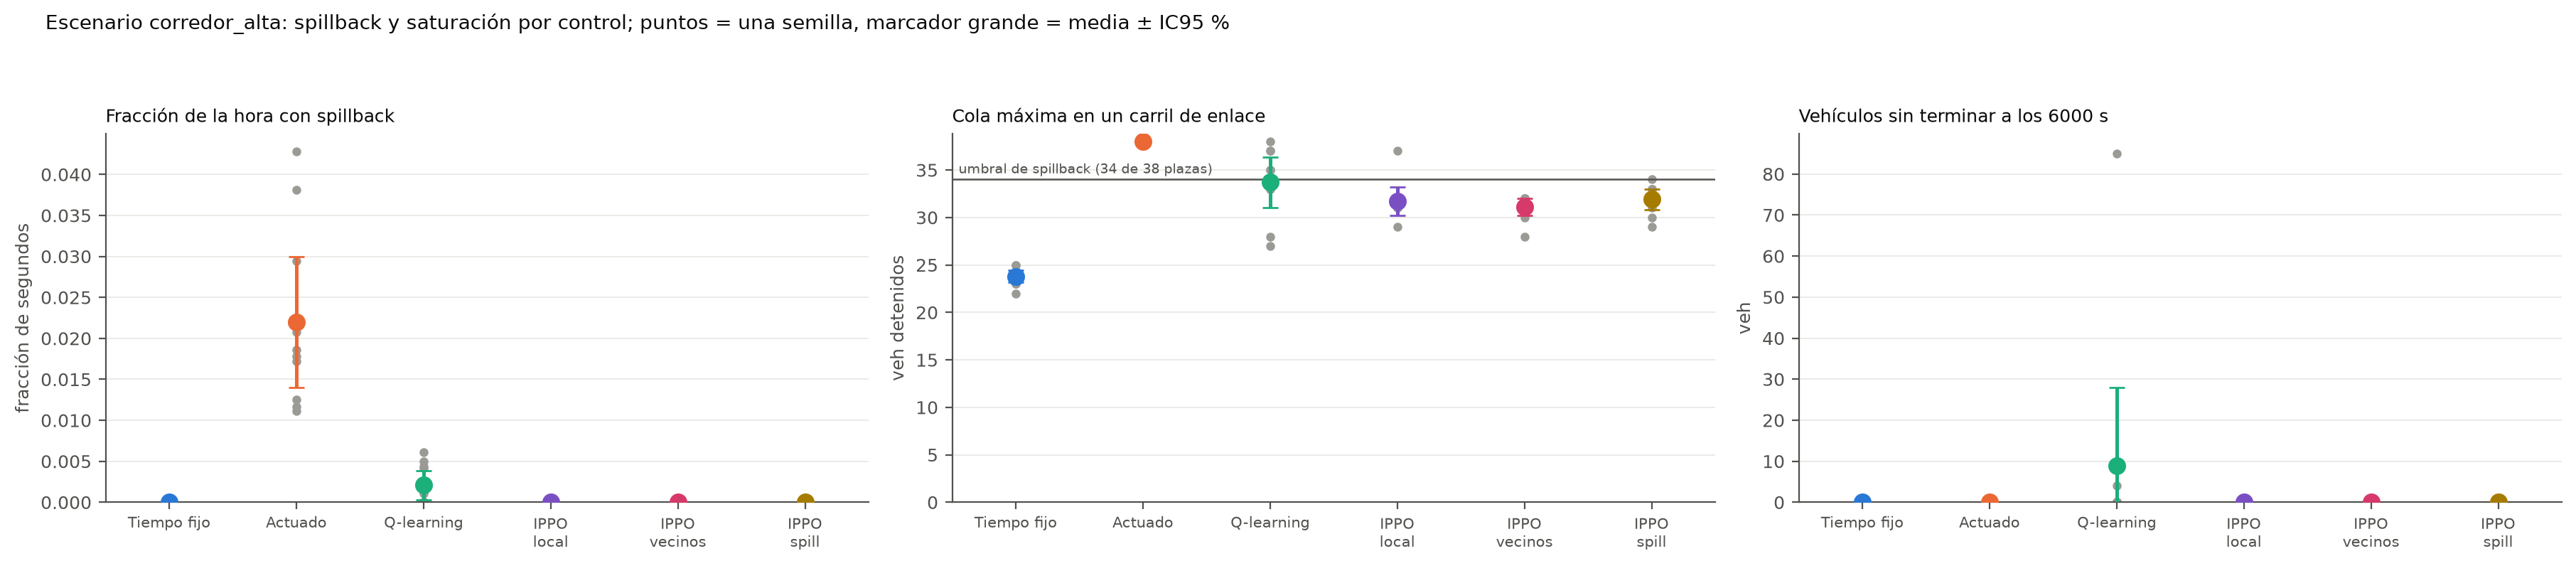
\includegraphics[width=0.95\textwidth]{fig_corredor_alta_spillback.png}
  \caption{Escenario corredor\_alta: fracción de la hora con \textit{spillback}, cola máxima en un carril del enlace y vehículos sin terminar, por control y semilla.}
  \label{fig:corredor-alta-spillback}
\end{figure}

\subsection*{Nivel alcanzado según el criterio prefijado}

El plan de pruebas fijó siete niveles de éxito antes de entrenar
(Sección~\ref{sec:plan}). Se alcanzan los siguientes:

\begin{itemize}
  \item \textbf{N0, medición:} regresión, determinismo y prueba de humo
    superados, la última después de tres correcciones registradas.
  \item \textbf{N1, estabilidad:} se cumple a medias, y conviene
    separar sus dos exigencias. La del signo se cumple para
    \emph{vecinos} en corredor y corredor\_alta, donde sus tres políticas
    quedan del mismo lado del tiempo fijo; en red las tres empatan con el
    fijo tuneado ($-0.5$, $-0.2$ y $+0.5$\,\%, ninguna significativa), de
    modo que no hay signo que estabilizar. La del
    rango no se cumple en sentido estricto en ningún caso: el rango
    entre políticas supera al intervalo de confianza de una sola en
    todos ellos, aunque por poco en \emph{vecinos} de red (0.20~s de
    rango frente a intervalos de 0.13 a 0.28~s) y por bastante en
    \emph{vecinos} de corredor (0.54 frente a 0.36 a 0.40~s). Donde la
    inestabilidad es grande es en \emph{local} de red, con 2.1~s de
    rango frente a intervalos de 0.20 a 0.37~s, y en \emph{spill} de
    corredor\_alta, con 4.3~s frente a 1.6 a 2.1~s. La lectura es que
    la mensajería hace el entrenamiento más repetible pero no lo
    vuelve indiferente a la semilla base, y que tres políticas por
    variante son el mínimo para detectarlo, no un número suficiente
    para caracterizar la dispersión.
  \item \textbf{N2, algoritmo:} \emph{local} tiene menos retraso que
    Q-learning en cruce, red, corredor y corredor\_alta, con intervalos
    que excluyen el cero y $p = 0.002$ en todos; se declara como
    comparación de paquete completo.
  \item \textbf{N3, coordinación:} se cumple a medias. \emph{vecinos}
    tiene menos retraso que \emph{local} con signo estable en tres de
    tres en red y corredor, y la fracción de vehículos de paso con a lo
    sumo una parada y el retraso en el sentido punta no son peores que
    los del fijo en ninguno de los dos; pero en red no queda por debajo
    de la onda verde tuneada, la iguala (intervalo $-0.3$ a $+1.3$\,\%),
    y el criterio pedía un intervalo que excluyera los valores positivos.
    Frente al fijo de 20/20 de la primera ronda sí lo cumplía.
  \item \textbf{N4, \textit{spillback}:} no se cumple. Todas las
    variantes IPPO tienen tasa cero en corredor\_alta, pero \emph{spill}
    no reduce la cola del enlace frente a \emph{vecinos}.
  \item \textbf{N5, práctico:} se cumple en cruce, corredor y
    corredor\_alta, y no en red. \emph{local} supera al actuado en cruce
    ($-2.6$\,\%, intervalo $-3.2$ a $-2.0$) y en corredor queda
    $1.7$\,\% por encima con intervalo que no incluye el cero;
    \emph{vecinos} lo supera en corredor ($-5.1$\,\%) y lo iguala en
    corredor\_alta ($-1.3$\,\%, intervalo que incluye el cero); en red
    queda $2.2$\,\% por encima, con intervalo que no incluye el cero.
  \item \textbf{N6, meta de la tesis:} $-25$\,\% de retraso frente al
    fijo se cumple solo en cruce ($-35$\,\%). En corredor, frente al
    fijo de reparto tuneado, \emph{vecinos} queda en $-6$\,\% (frente
    al fijo simétrico original la cifra era $-38$\,\%); en
    corredor\_alta se queda en $-20$ a $-23$\,\% y en red, donde el
    propio actuado solo consigue $-2$\,\%, empata con el fijo
    ($+0.5$\,\%). Las metas de
    colas y CO$_2$ se cumplen en cruce; en corredor ya no ($-6$ y
    $-2$\,\% frente al fijo tuneado); la de CO$_2$ se cumple también en
    corredor\_alta ($-11$ a $-12$\,\% en las siete políticas), donde
    la de colas no ($-1$ a $-7$\,\%); la de \textit{throughput} no la
    alcanza ningún control.
  \item \textbf{Robustez:} con latencia de 5~s y pérdida del 30\,\%, la
    política de \emph{vecinos} pierde 0.8~s en red (dentro del límite de
    2~s) y 2.2~s en corredor (fuera por poco), y en ambos casos la
    progresión se deshace.
\end{itemize}

\section{Lectura conjunta}
\label{sec:lectura}

\noindent\textbf{Qué optimiza el agente y qué mide la meta.} La recompensa de la
Ecuación~\ref{eq:recompensa} penaliza vehículos detenidos y su espera.
Con la política congelada, el agente la mejora un $26$\,\% frente al
fijo en cruce y la empeora en cruce2, red y corredor. Pero la meta de
la tesis es el retraso, que además de la detención incluye frenadas,
aceleraciones y avance lento en cola, y las dos magnitudes no se mueven
juntas. En cruce la espera baja un $26$\,\% y el retraso solo un
$6$\,\%; en red la espera sube un $4$\,\% mientras el retraso sube un
$15$\,\%; y en el corredor, frente al fijo simétrico de la primera
ronda, la espera bajaba un $13$\,\% mientras el retraso subía un
$6$\,\%. La diferencia son las paradas adicionales que provoca un agente
que cambia de fase entre un $13$ y un $77$\,\% más veces que el fijo:
las paradas por vehículo suben en los cinco casos. Alinear la recompensa
con la métrica primaria es lo que hace el módulo U4, cuya recompensa
sustituye la cola detenida por el retraso por segundo
(Sección~\ref{sec:u4}); la Sección~\ref{sec:resultados-u4} muestra el
efecto.

\noindent\textbf{Techo del método tabular.} Con dos fases y 512 estados el agente
visita 130 y converge; con cuatro fases y 1024 estados visita 390 y su
política congelada es peor que el fijo. La discretización en cuatro
niveles por aproximación, que hace posible la tabla Q, es también su
límite: es el argumento empírico para DQN y PPO en el módulo U2.

\noindent\textbf{Reacción local frente a coordinación.} En el corredor de dos
cruces los agentes independientes quedan un $60$\,\% por detrás del
fijo coordinado y con reparto tuneado; en la red de tres cruces quedan
un $15$\,\% por detrás de la onda verde, aunque muy por delante del
mismo programa sin desfases. Cuanto más larga es la cadena de
semáforos, más vale la progresión anticipada que la reacción a la cola
local. Es la evidencia que motiva el módulo U4 (estado extendido con
información de vecinos, mensajería y penalización por \textit{spillback}).

\noindent\textbf{El actuado como referencia exigente.} El control actuado de
SUMO, que no aprende y solo extiende el verde mientras detecta
vehículos, es mejor que el agente tabular en los cinco casos y cumple la
meta de $-25$\,\% de retraso en cruce; en el corredor empata con un fijo
cuyo reparto de verde se tuneó bien, que es otra forma de decir que un
fijo bien tuneado ya es un rival exigente. Cualquier resultado de RL que
se reporte en adelante debe compararse contra él y no solo contra el
tiempo fijo.

\noindent\textbf{Metas.} Con la política congelada y diez semillas, el agente
Q-learning no cumple la meta de retraso ($-25$\,\%) en ningún caso. La
de colas ($-20$\,\%) la alcanza en la media solo en cruce ($-23$\,\%),
con un intervalo que no excluye el $-20$\,\%. La de CO$_2$ ($-5$\,\%) no
la alcanza en ninguno: $-1.5$\,\% en cruce y aumentos en los demás. La
meta de \textit{throughput} no es evaluable en los cuatro escenarios
nominales: en ellos todos los vehículos completan su viaje bajo los
tres controles y solo entre un 2 y un 3\,\% llega después de los
3600~s, sea cual sea el control; el corredor con demanda doble, en la
Sección~\ref{sec:resultados-u4}, es el único donde discrimina.

\section{Limitaciones de esta fase}

Los cinco escenarios son sintéticos y el cruce real de Lima sigue
pendiente. Las llegadas son equiespaciadas, por lo que la variabilidad
entre semillas es solo la del comportamiento de los conductores y los
intervalos de confianza son estrechos; con llegadas aleatorias los
controles de referencia empeoran y habría que repetir barridos y
entrenamientos. Para el agente tabular hay una sola corrida de
entrenamiento por escenario, de modo que su varianza entre
entrenamientos con distinta semilla base no está medida; el caso del
corredor, donde dos entrenamientos que solo diferían en el reloj de
decisión dieron 25.8 y 33.9~s de retraso, indica que esa varianza no
es pequeña, y por eso el módulo U4 entrena tres políticas por
variante. La referencia fija del corredor se rehízo tras la revisión
adversarial del documento, cuando se comprobó que el barrido original
no variaba el reparto de verde; el episodio muestra que la magnitud de
cualquier mejora reportada depende de lo bien tuneada que esté la
referencia, y que conviene someterla a un intento de refutación antes
de publicarla. La comparación entre IPPO y Q-learning es de paquete
completo (estado, recompensa y algoritmo cambian a la vez); aislar el
efecto de la recompensa exigiría reentrenar el agente tabular con el
retraso por segundo, lo que queda pendiente. SARSA y DQN, las llegadas
aleatorias y el cruce real de Lima son los siguientes casos del plan de
pruebas.
